\begin{figure}[b]
    \centering
    \begin{subfigure}{0.4\textwidth}
        \centering
        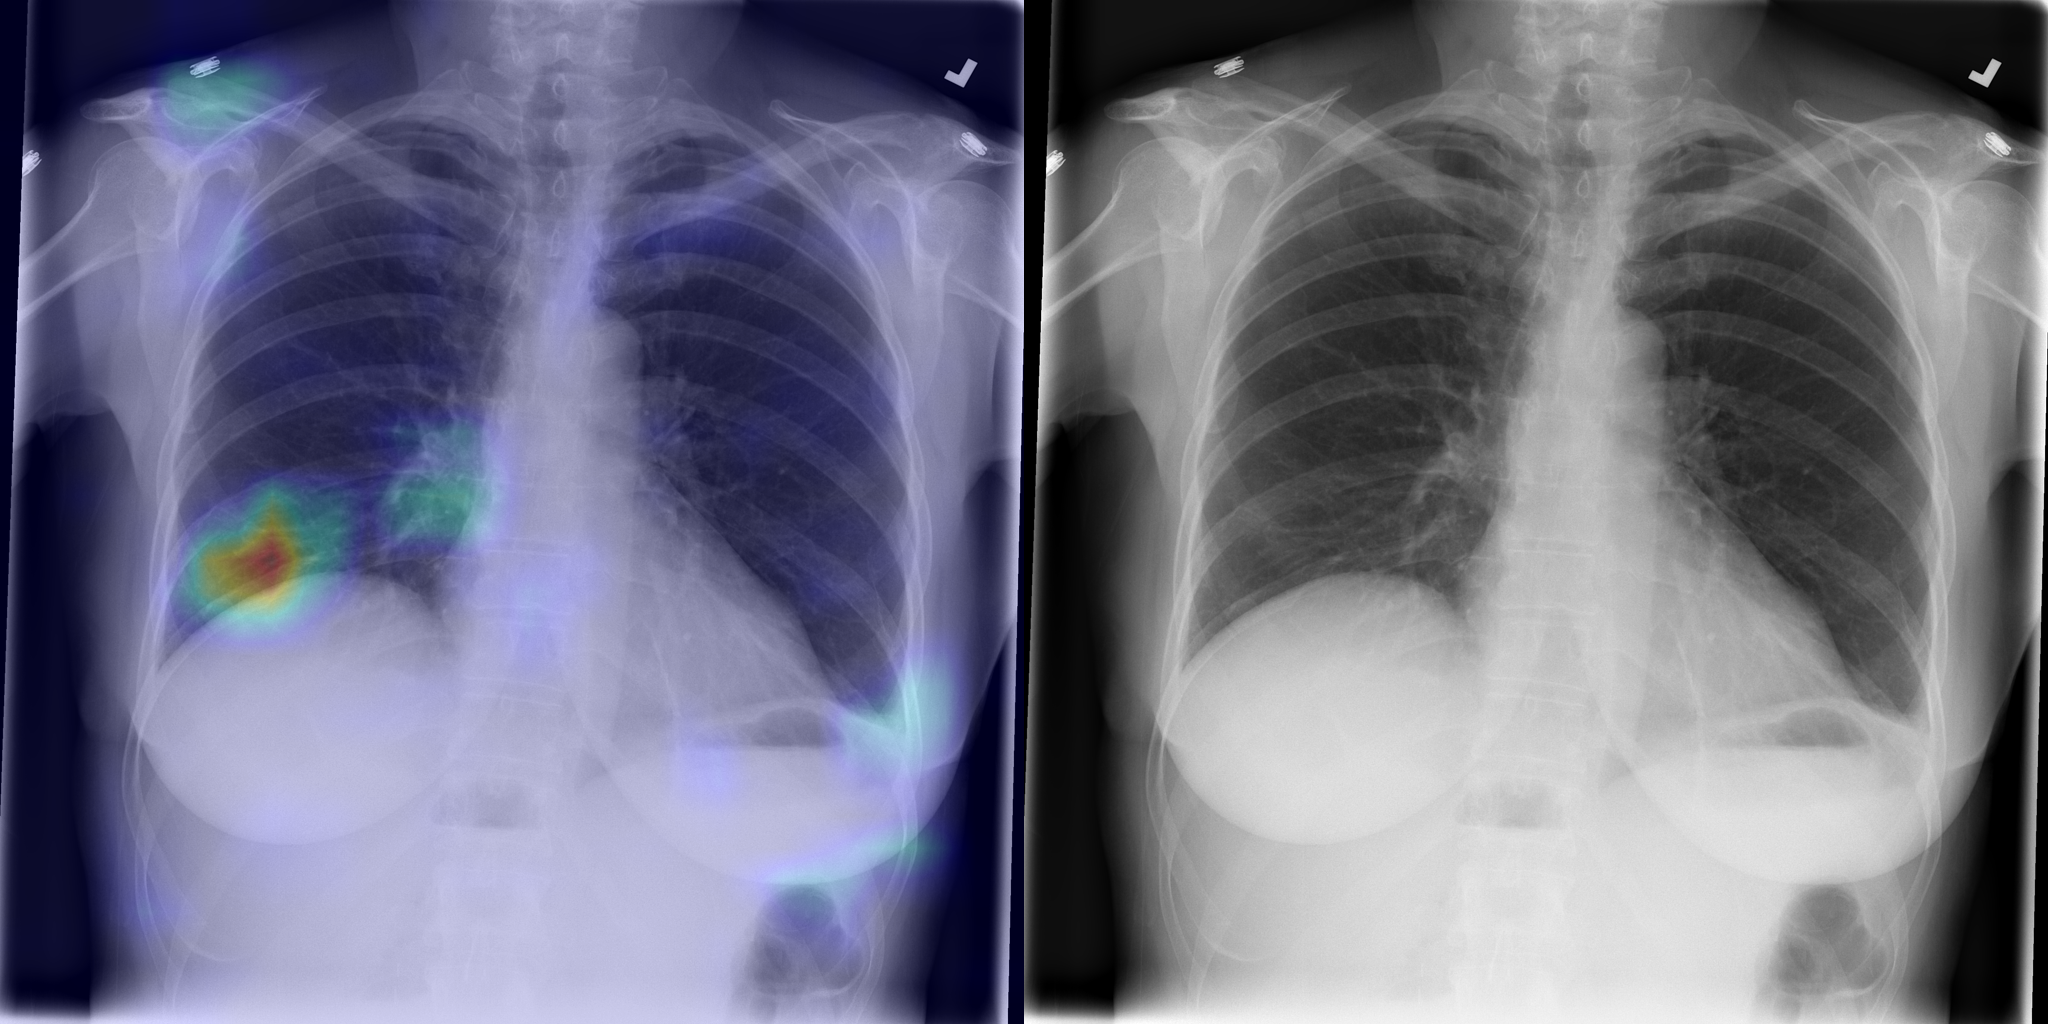
\includegraphics[width=1.0\textwidth]{Chapters/5. Conclusiones/img/Atelectasis/1_1_00000147_001.png}
    \end{subfigure}
    \begin{subfigure}{0.4\textwidth}
        \centering
        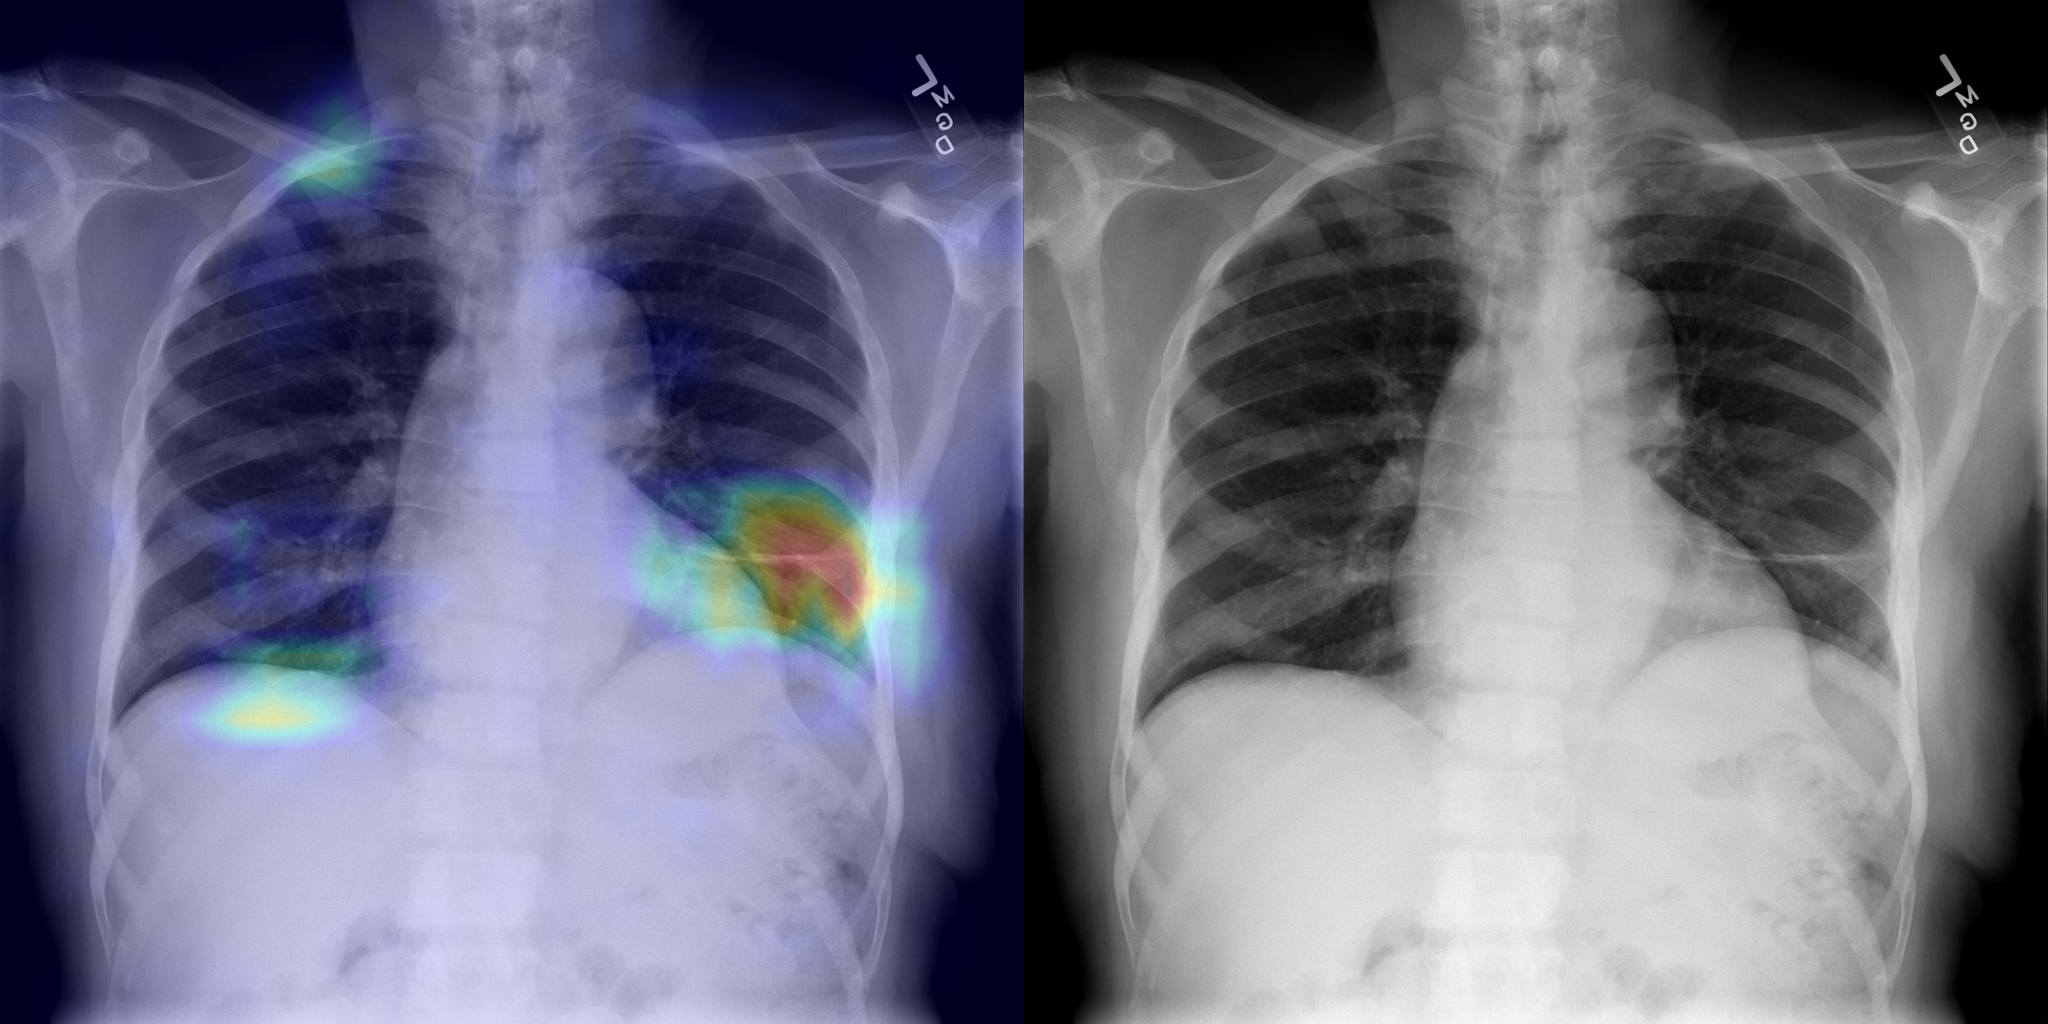
\includegraphics[width=1.0\textwidth]{Chapters/5. Conclusiones/img/Atelectasis/1_1_00000149_002.png}
    \end{subfigure}
    \begin{subfigure}{0.4\textwidth}
        \centering
        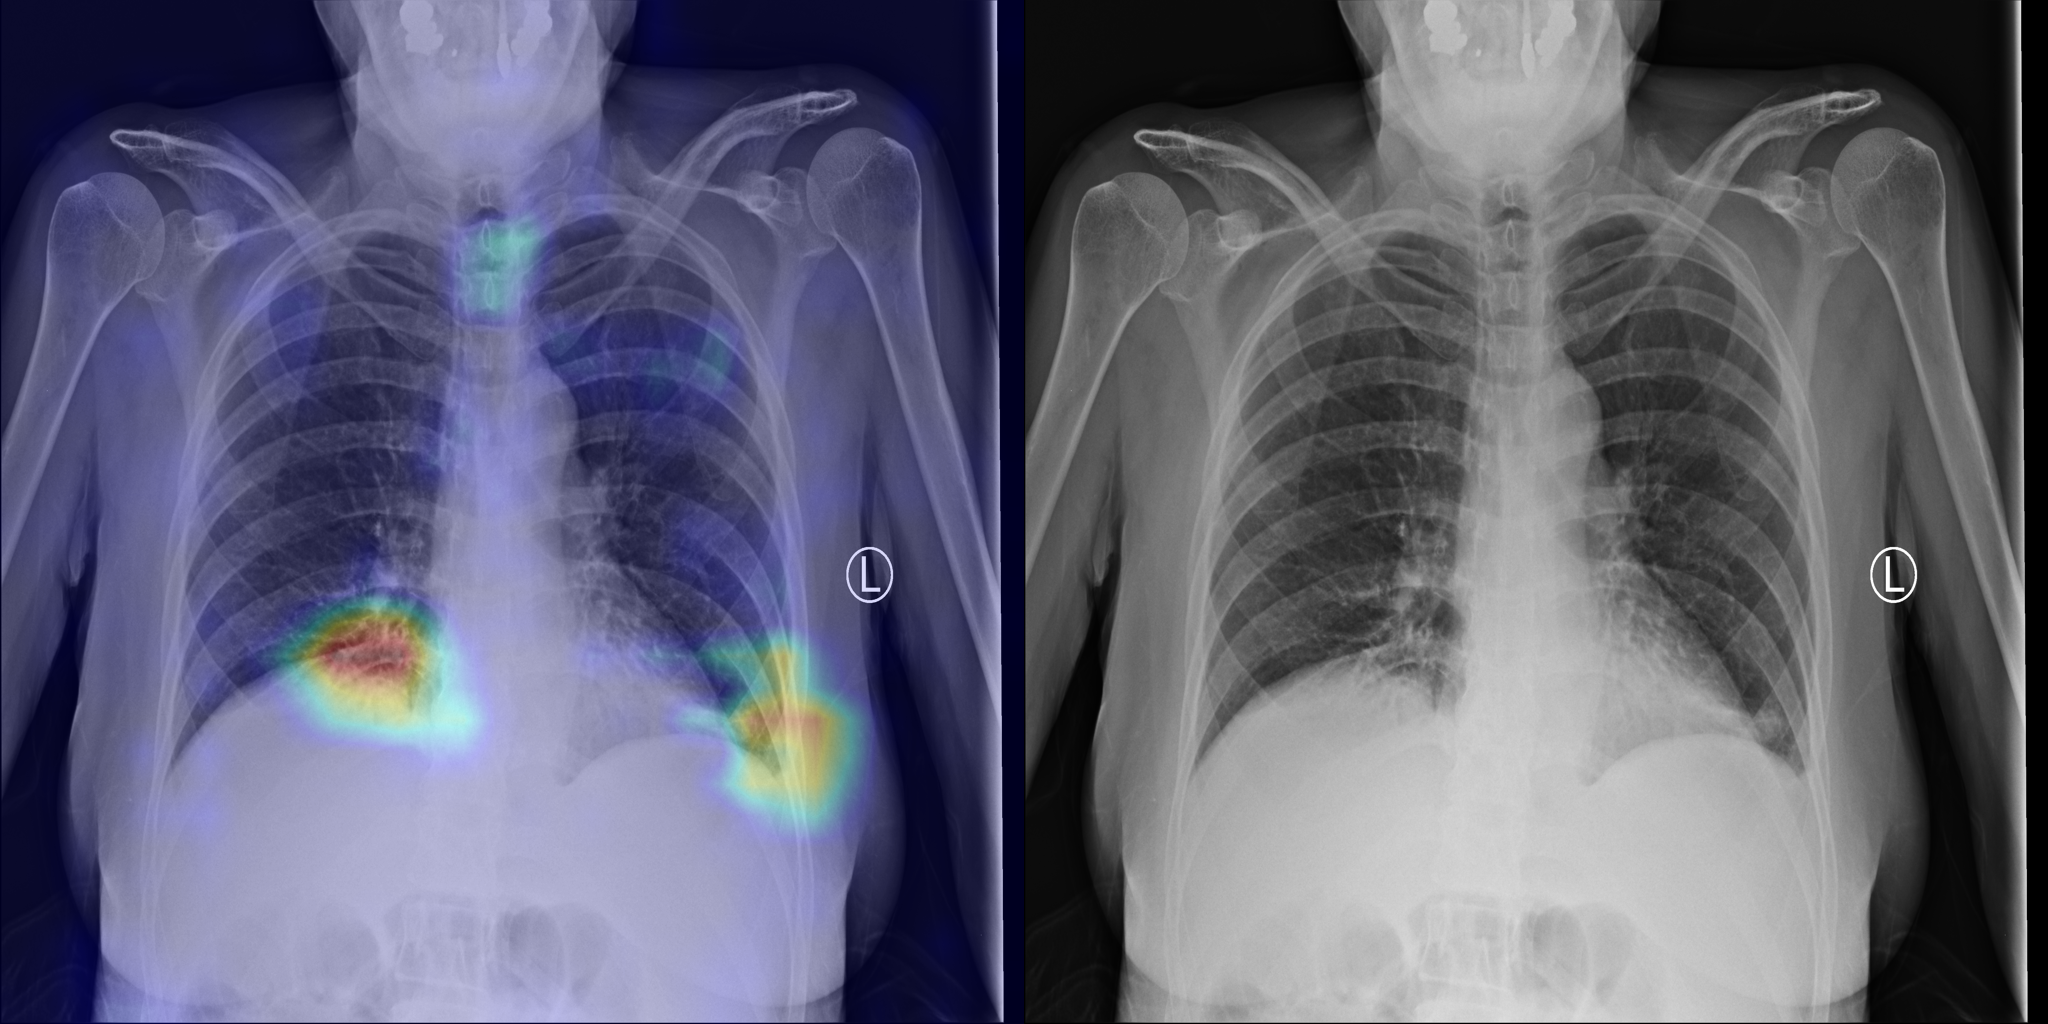
\includegraphics[width=1.0\textwidth]{Chapters/5. Conclusiones/img/Atelectasis/1_1_00000150_003.png}
    \end{subfigure}
    \begin{subfigure}{0.4\textwidth}
        \centering
        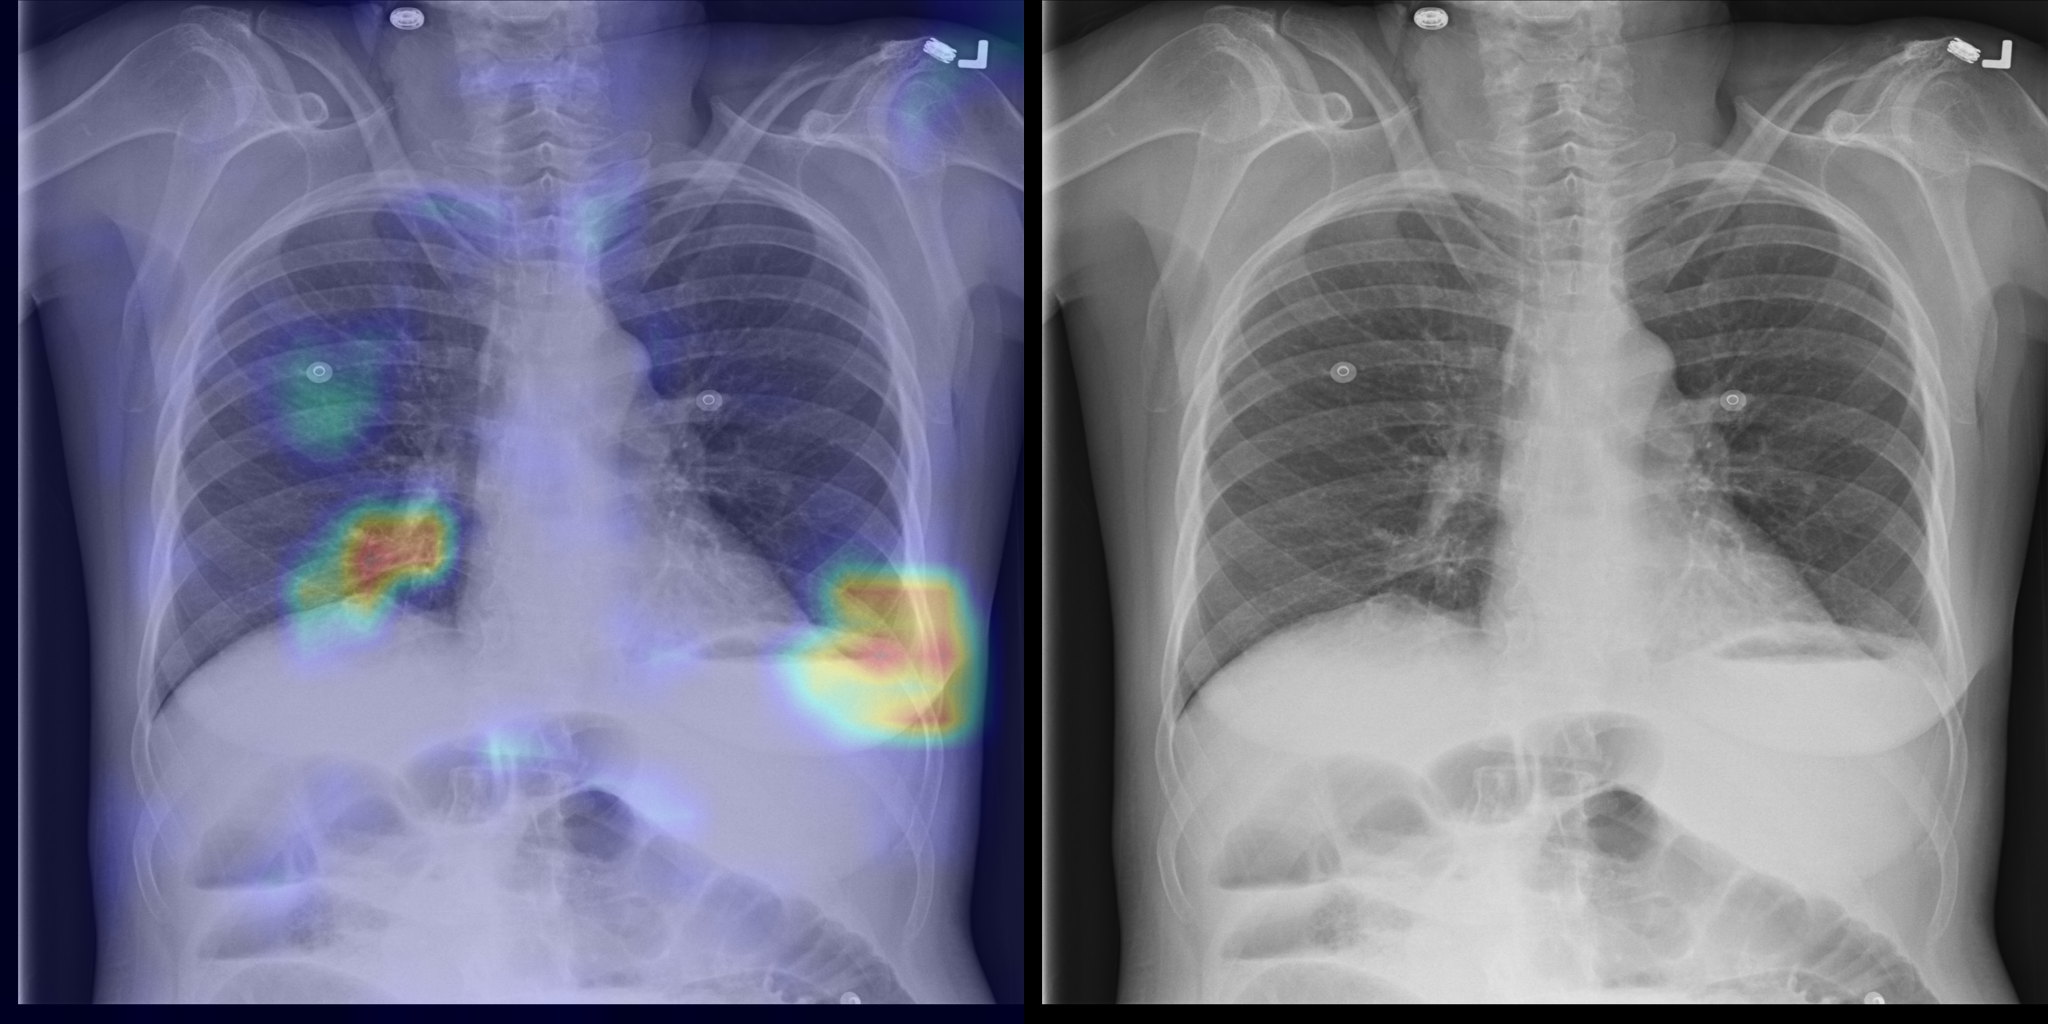
\includegraphics[width=1.0\textwidth]{Chapters/5. Conclusiones/img/Atelectasis/1_1_00000150_004.png}
    \end{subfigure}
    \begin{subfigure}{0.4\textwidth}
        \centering
        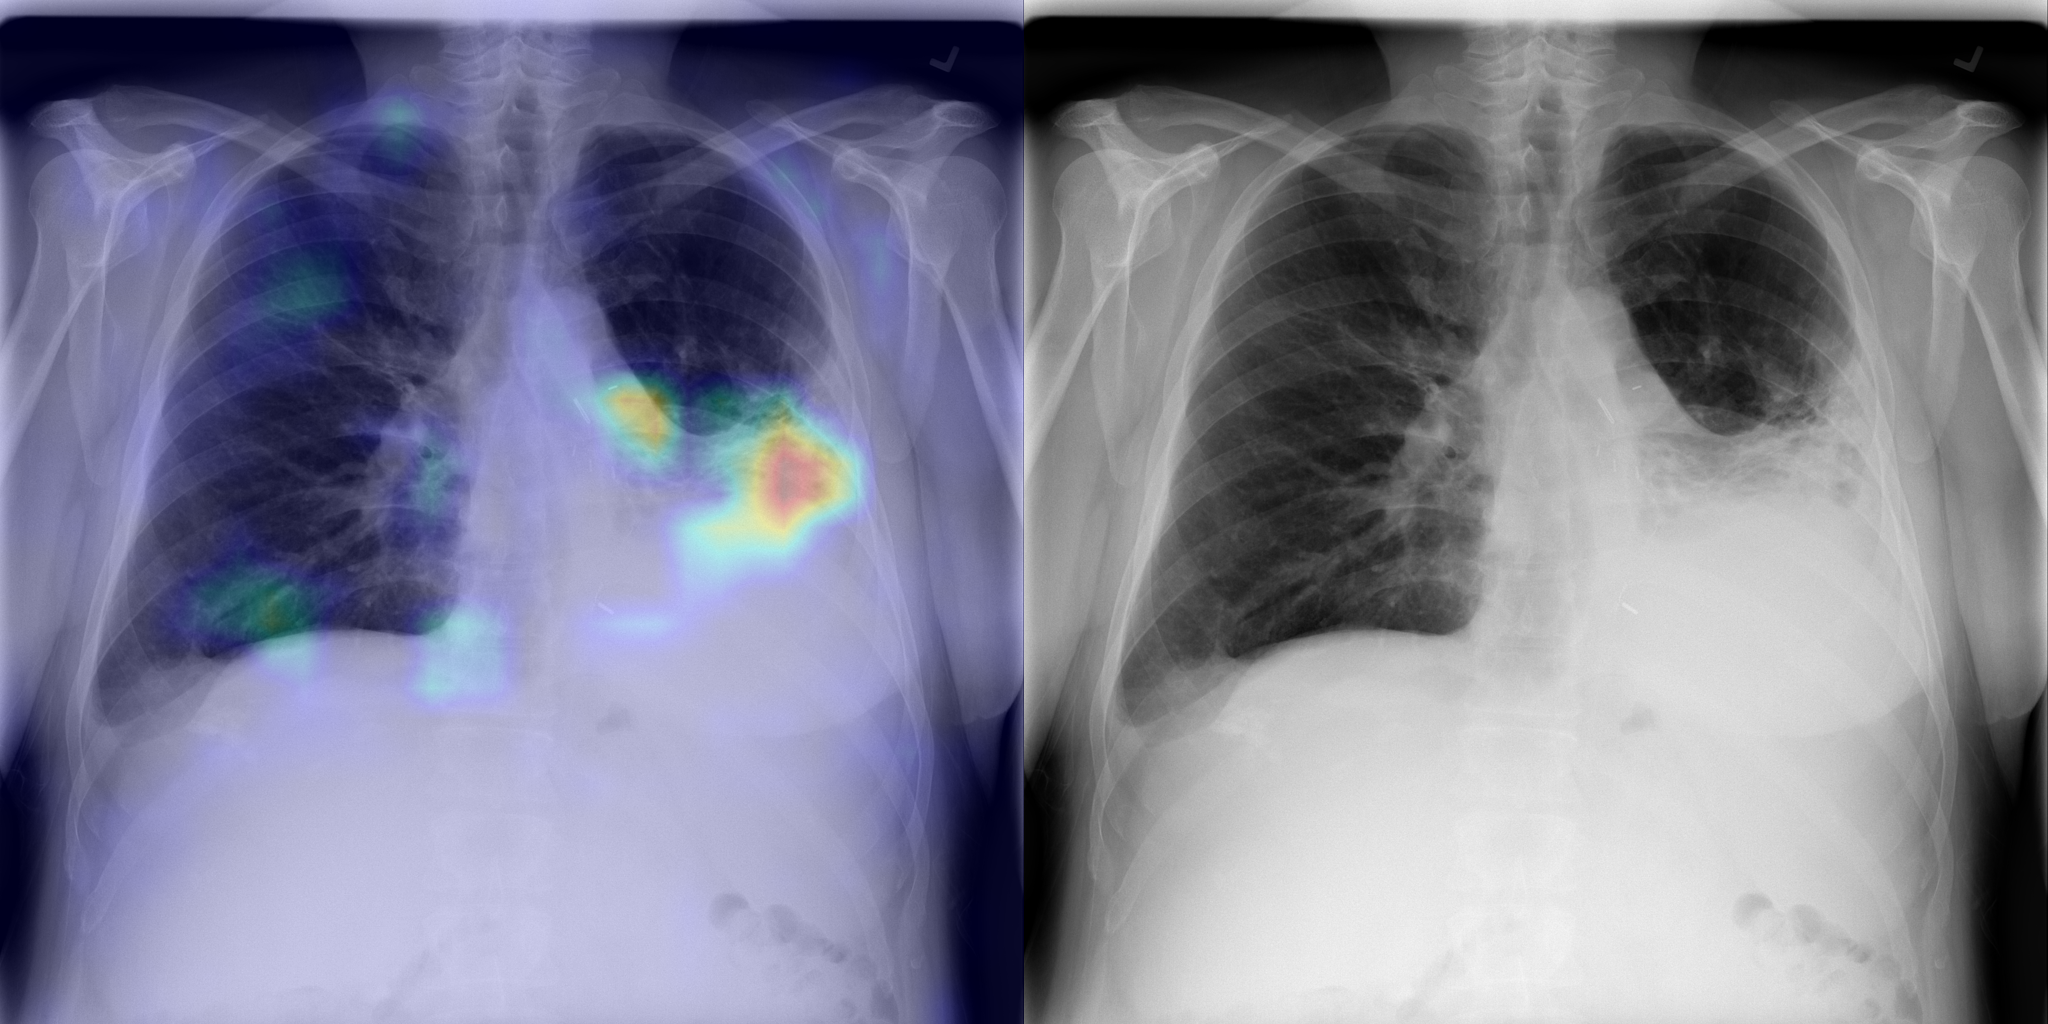
\includegraphics[width=1.0\textwidth]{Chapters/5. Conclusiones/img/Atelectasis/1_1_00000467_000.png}
    \end{subfigure}
    \begin{subfigure}{0.4\textwidth}
        \centering
        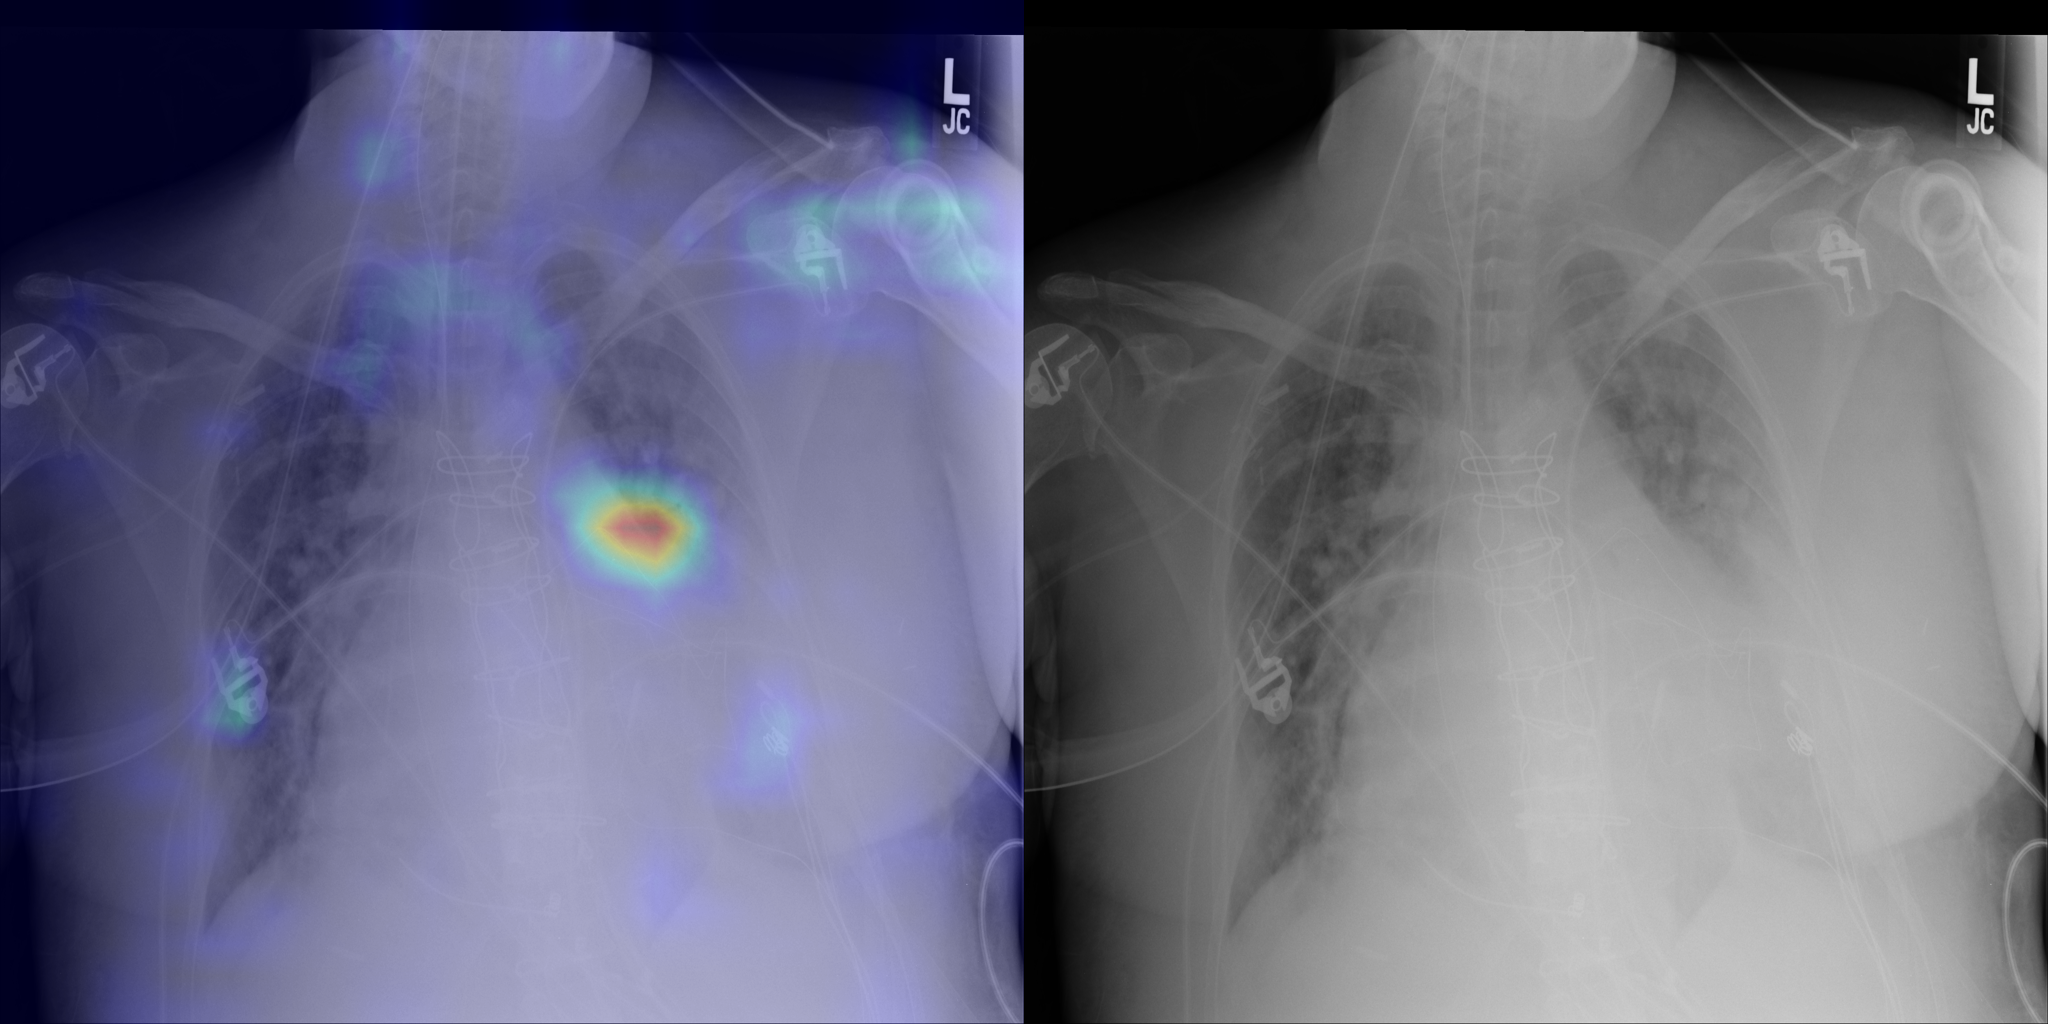
\includegraphics[width=1.0\textwidth]{Chapters/5. Conclusiones/img/Atelectasis/1_1_00000032_036.png}
    \end{subfigure}
    \begin{subfigure}{0.4\textwidth}
        \centering
        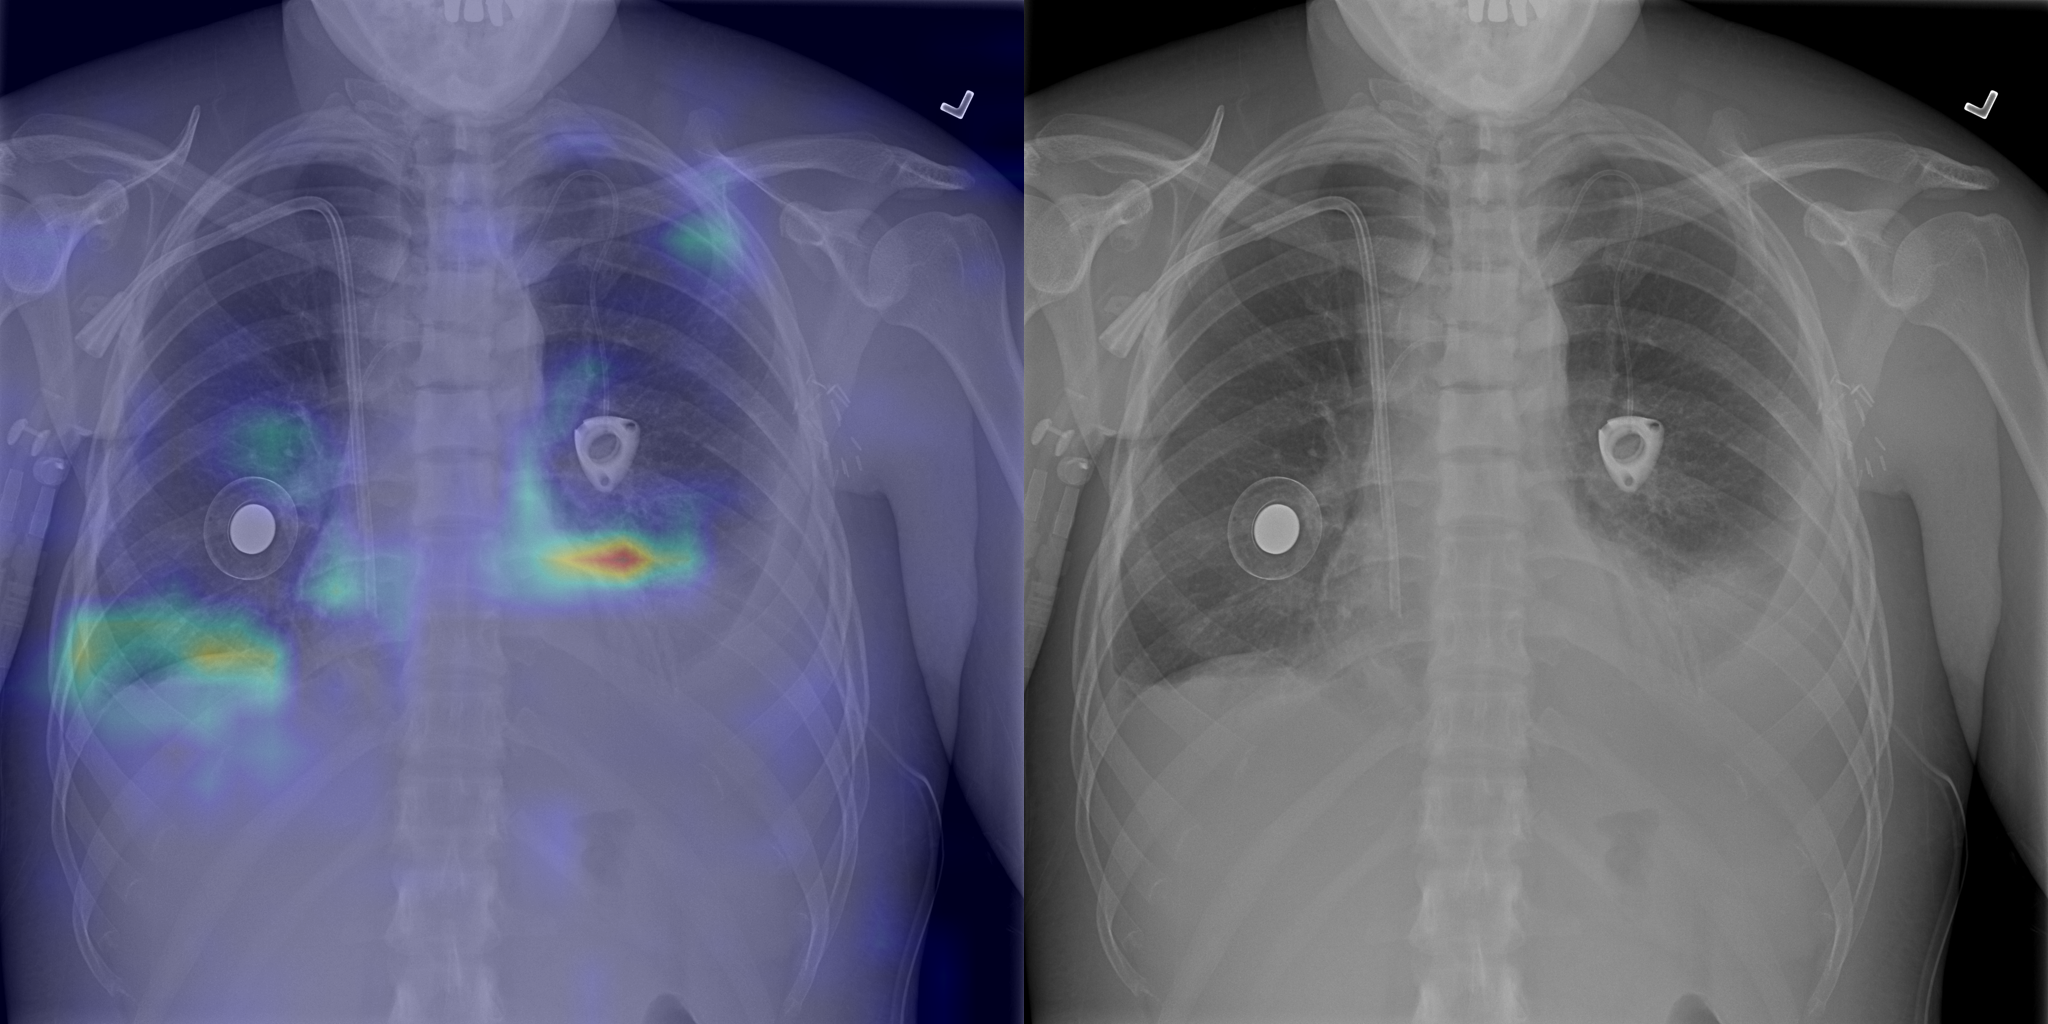
\includegraphics[width=1.0\textwidth]{Chapters/5. Conclusiones/img/Atelectasis/1_1_00029596_022.png}
    \end{subfigure}
    \begin{subfigure}{0.4\textwidth}
        \centering
        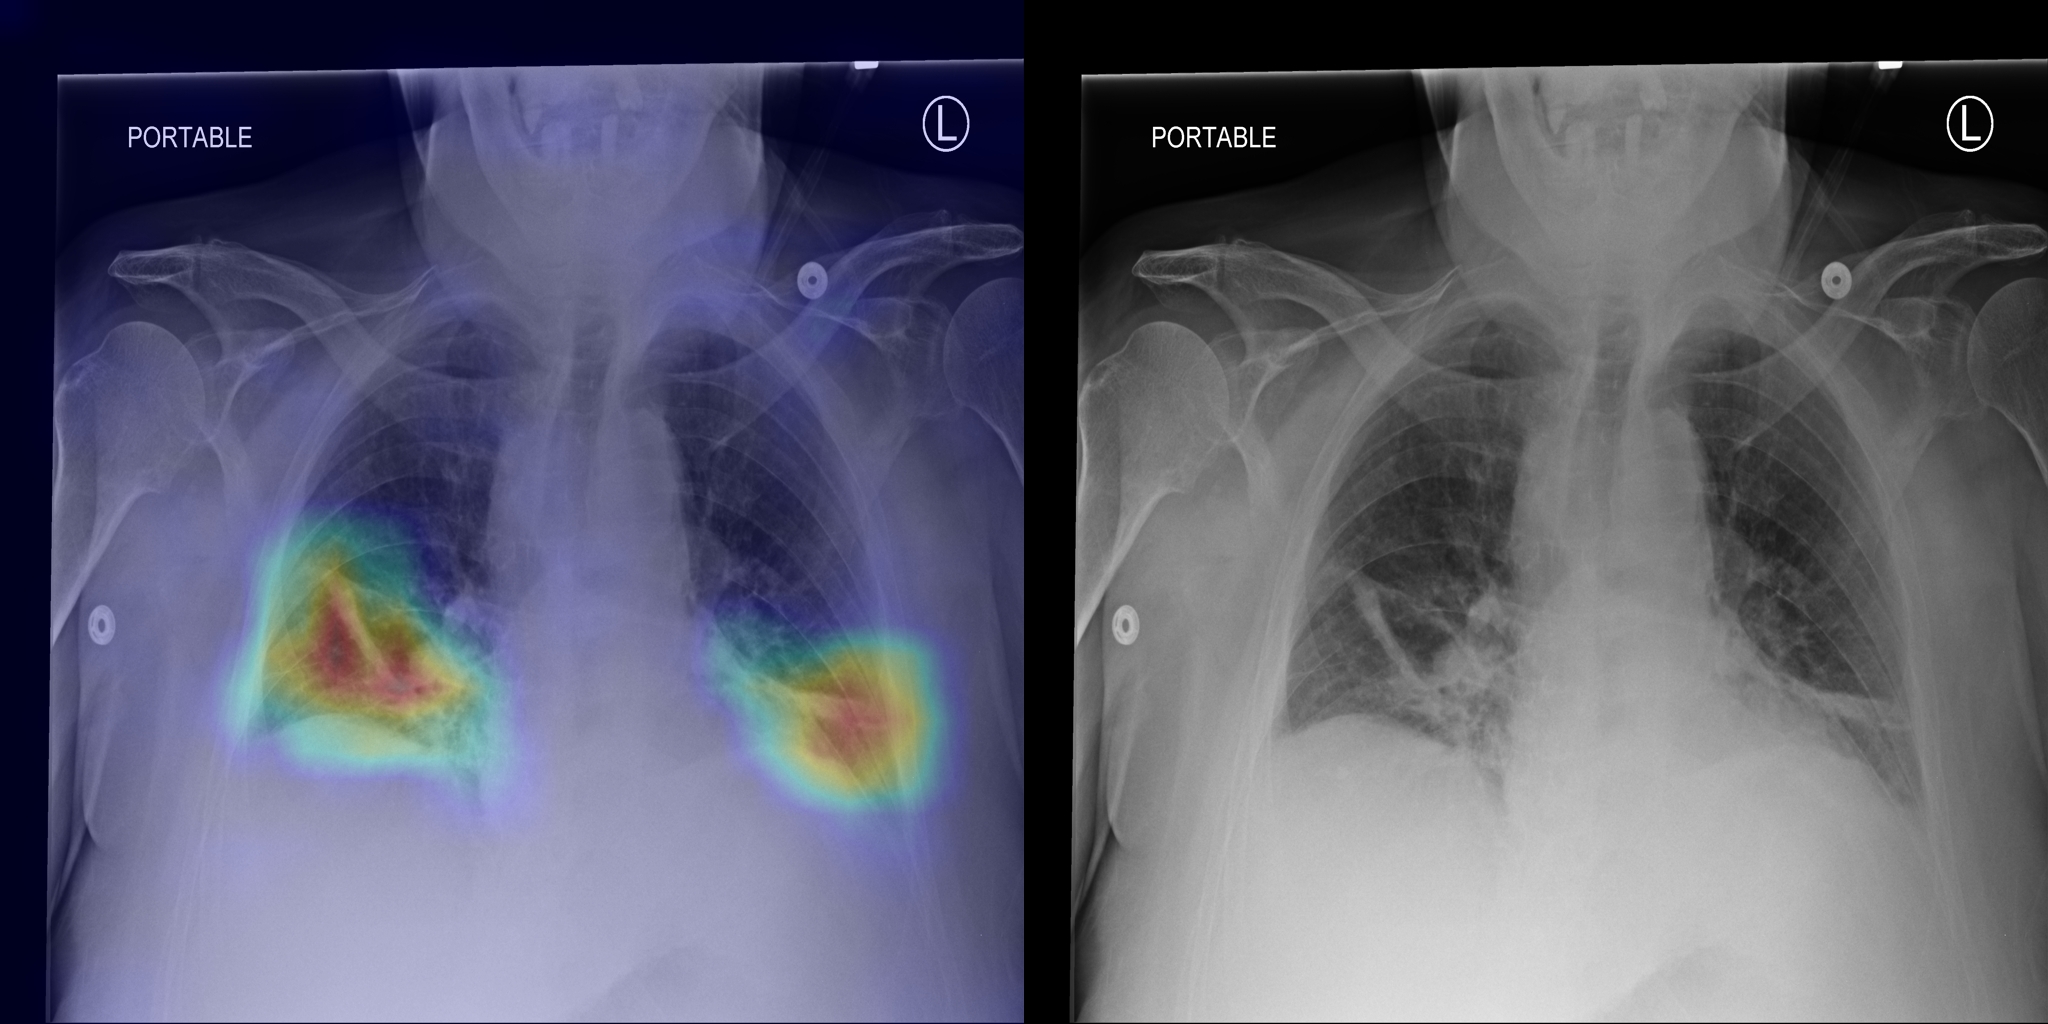
\includegraphics[width=1.0\textwidth]{Chapters/5. Conclusiones/img/Atelectasis/1_1_00030408_000.png}
    \end{subfigure}
    \begin{subfigure}{0.4\textwidth}
        \centering
        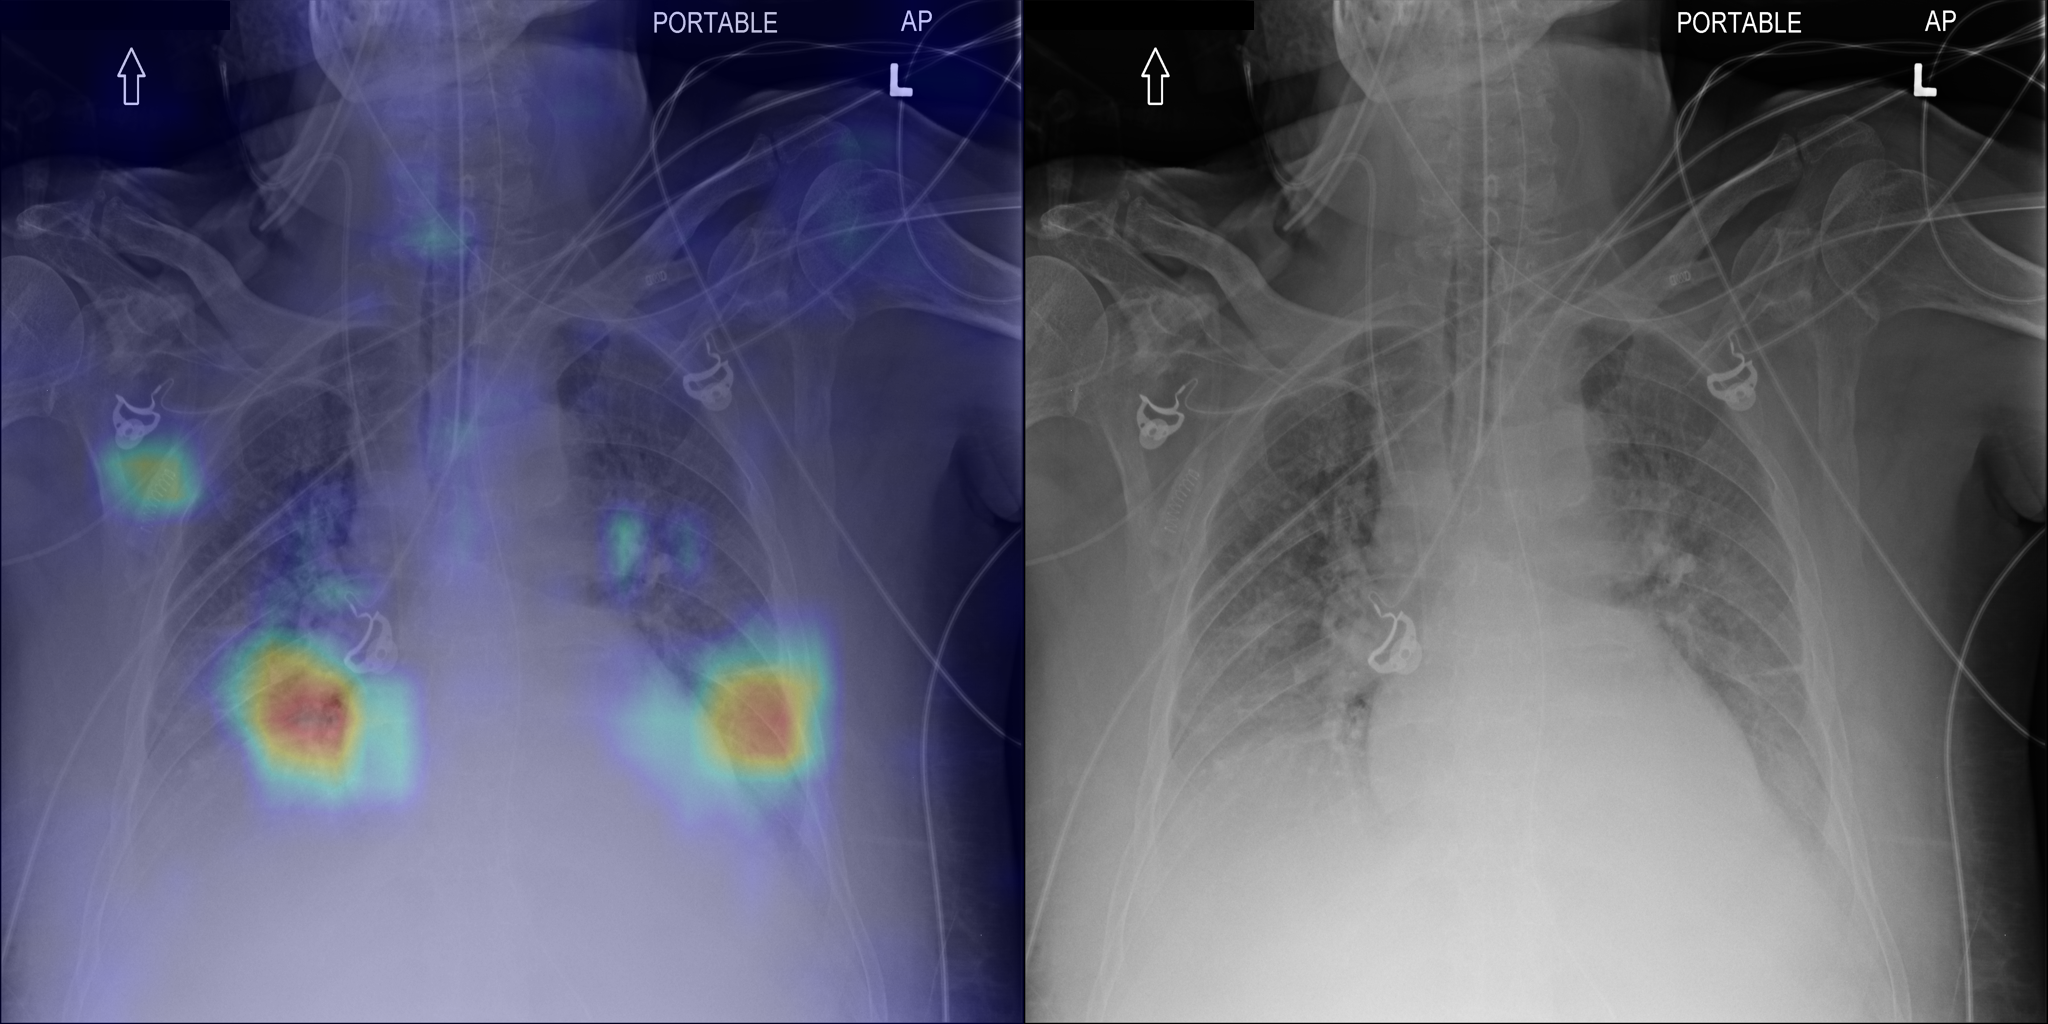
\includegraphics[width=1.0\textwidth]{Chapters/5. Conclusiones/img/Atelectasis/1_1_00030408_013.png}
    \end{subfigure}
    \begin{subfigure}{0.4\textwidth}
        \centering
        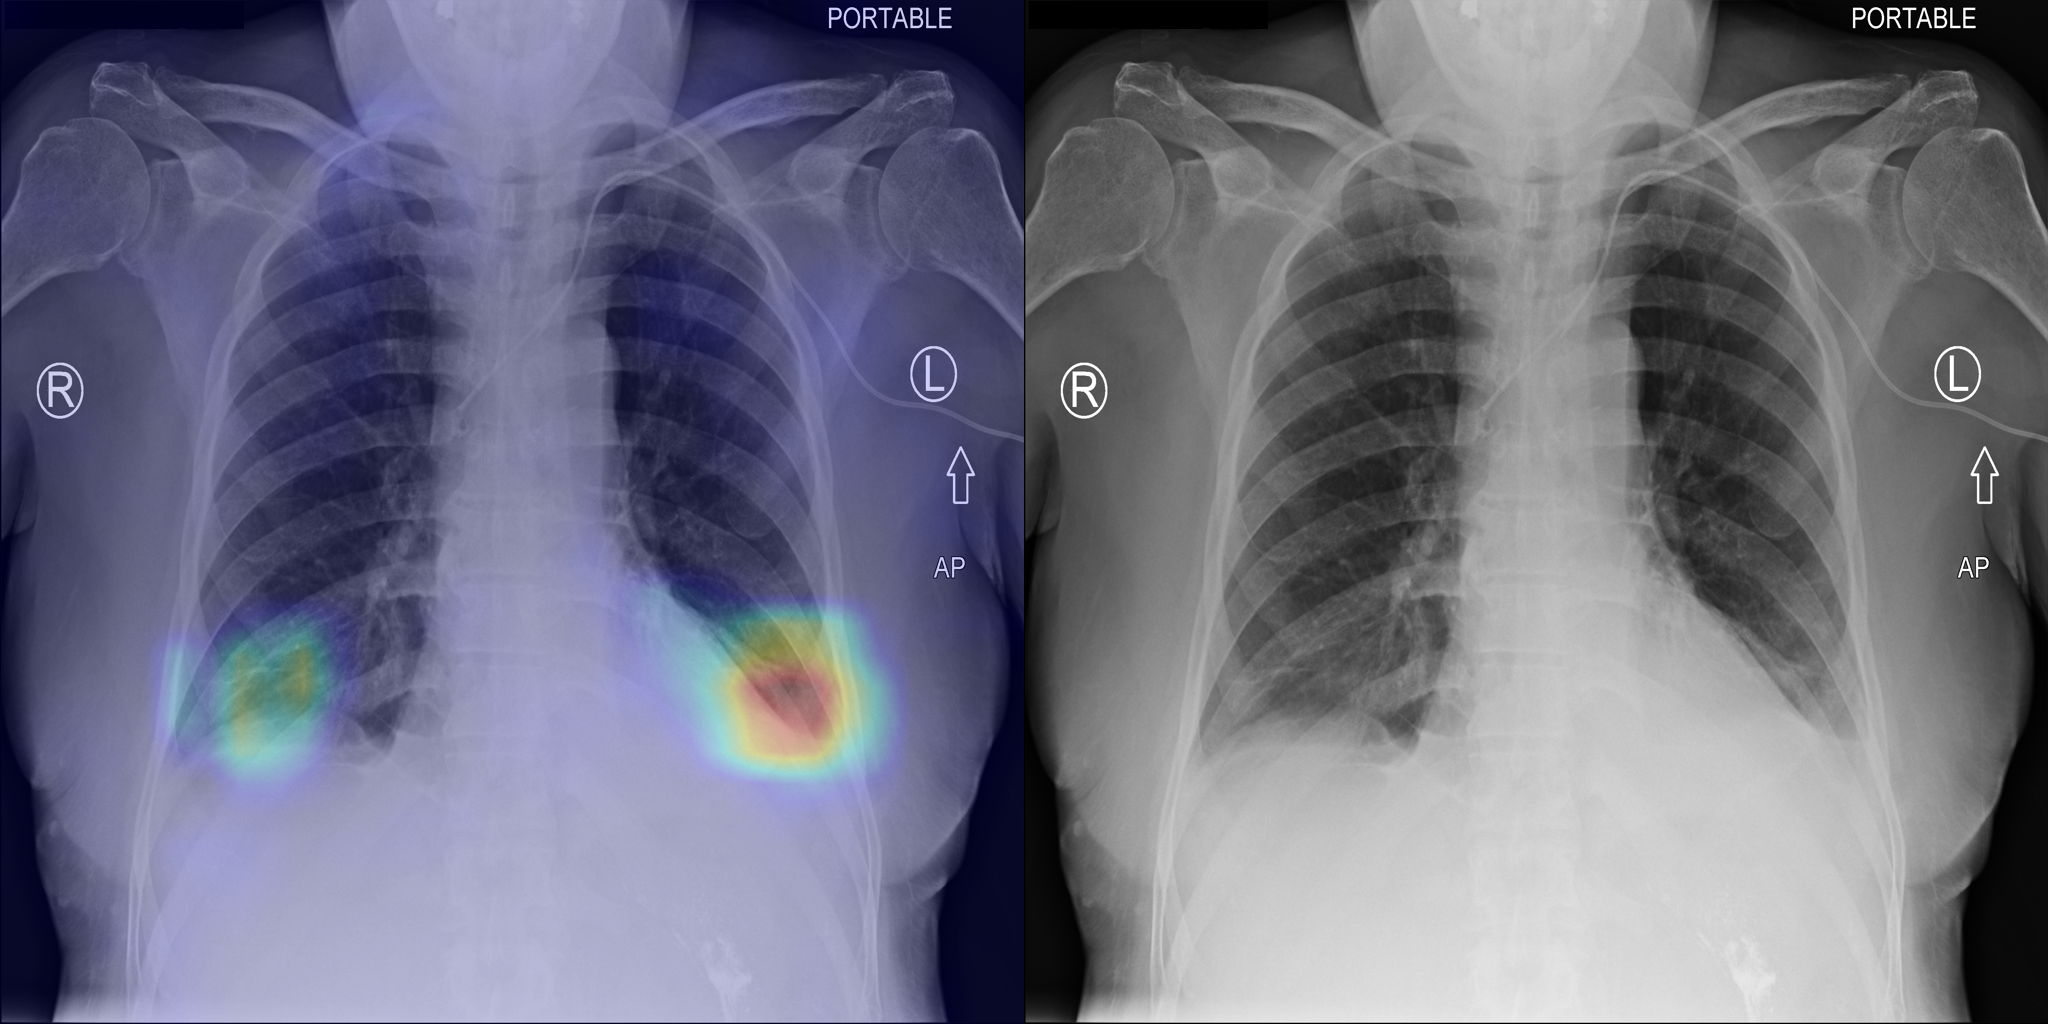
\includegraphics[width=1.0\textwidth]{Chapters/5. Conclusiones/img/Atelectasis/1_1_00028974_018.png}
    \end{subfigure}

    \caption[short]{Atelectasis. Radiografías detectadas con la patología de atelectasis por los
                    radiólogos. A la izquierda de cada imagen el GradCam correspondiente a la detección
                    de la patología como positivo por el modelo CNN.}
\end{figure}

\begin{figure}[b]
    \centering
    \begin{subfigure}{0.4\textwidth}
        \centering
        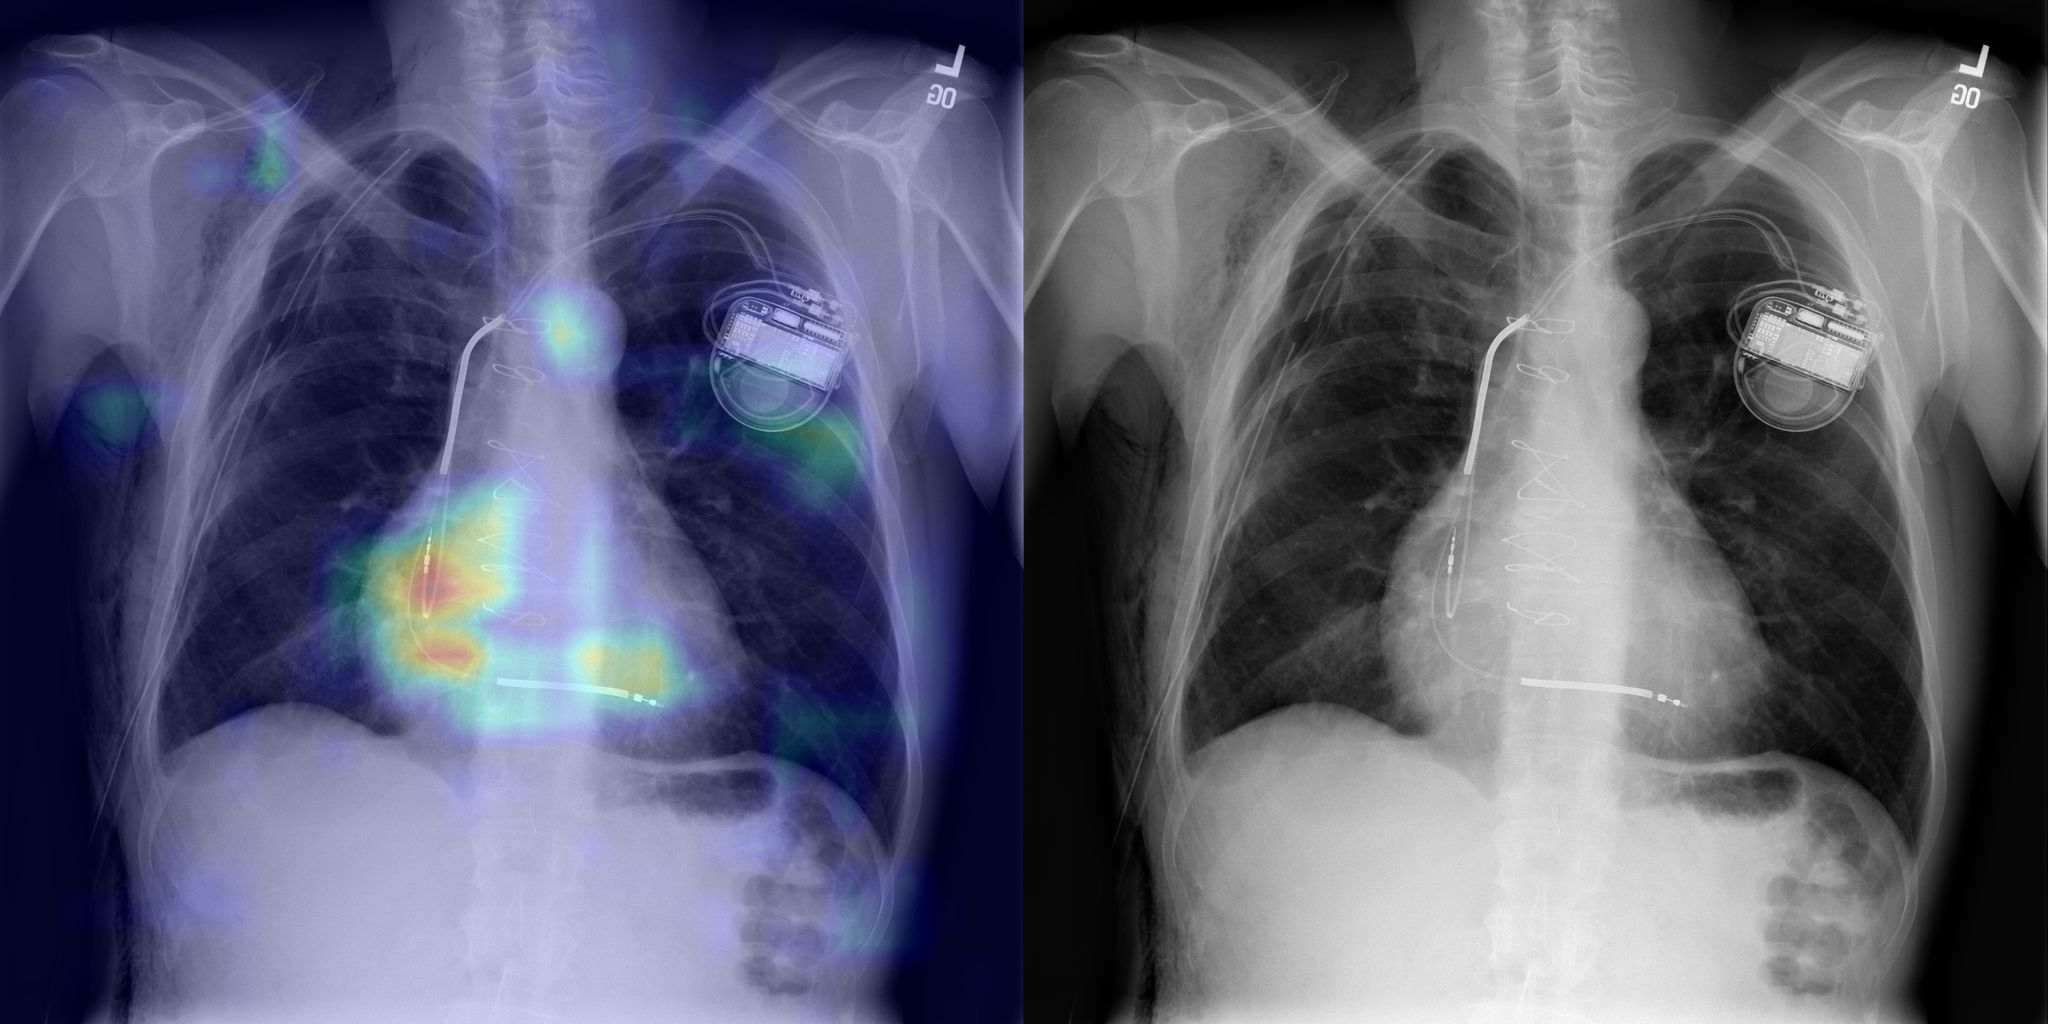
\includegraphics[width=1.0\textwidth]{Chapters/5. Conclusiones/img/Cardiomegaly/1_0_00000013_037.png}
    \end{subfigure}
    \begin{subfigure}{0.4\textwidth}
        \centering
        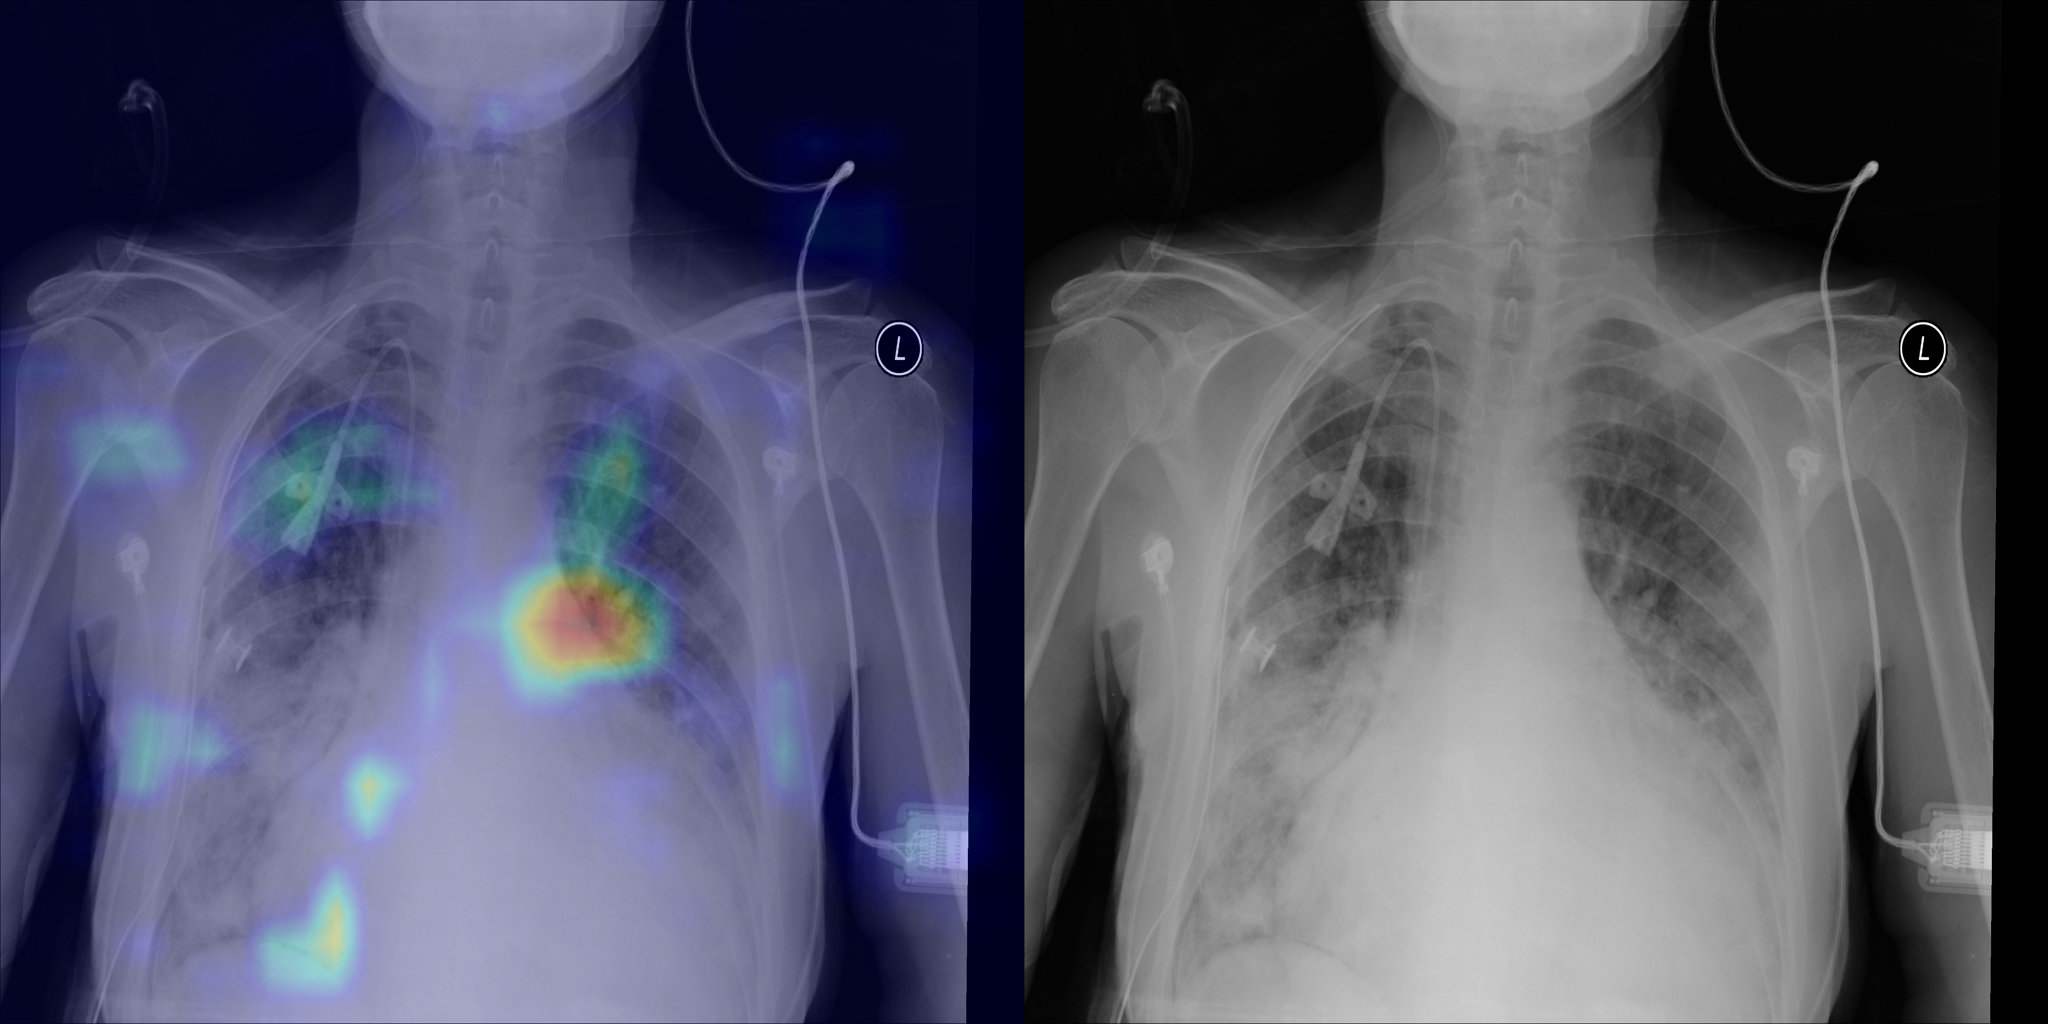
\includegraphics[width=1.0\textwidth]{Chapters/5. Conclusiones/img/Cardiomegaly/1_0_00000211_018.png}
    \end{subfigure}
    \begin{subfigure}{0.4\textwidth}
        \centering
        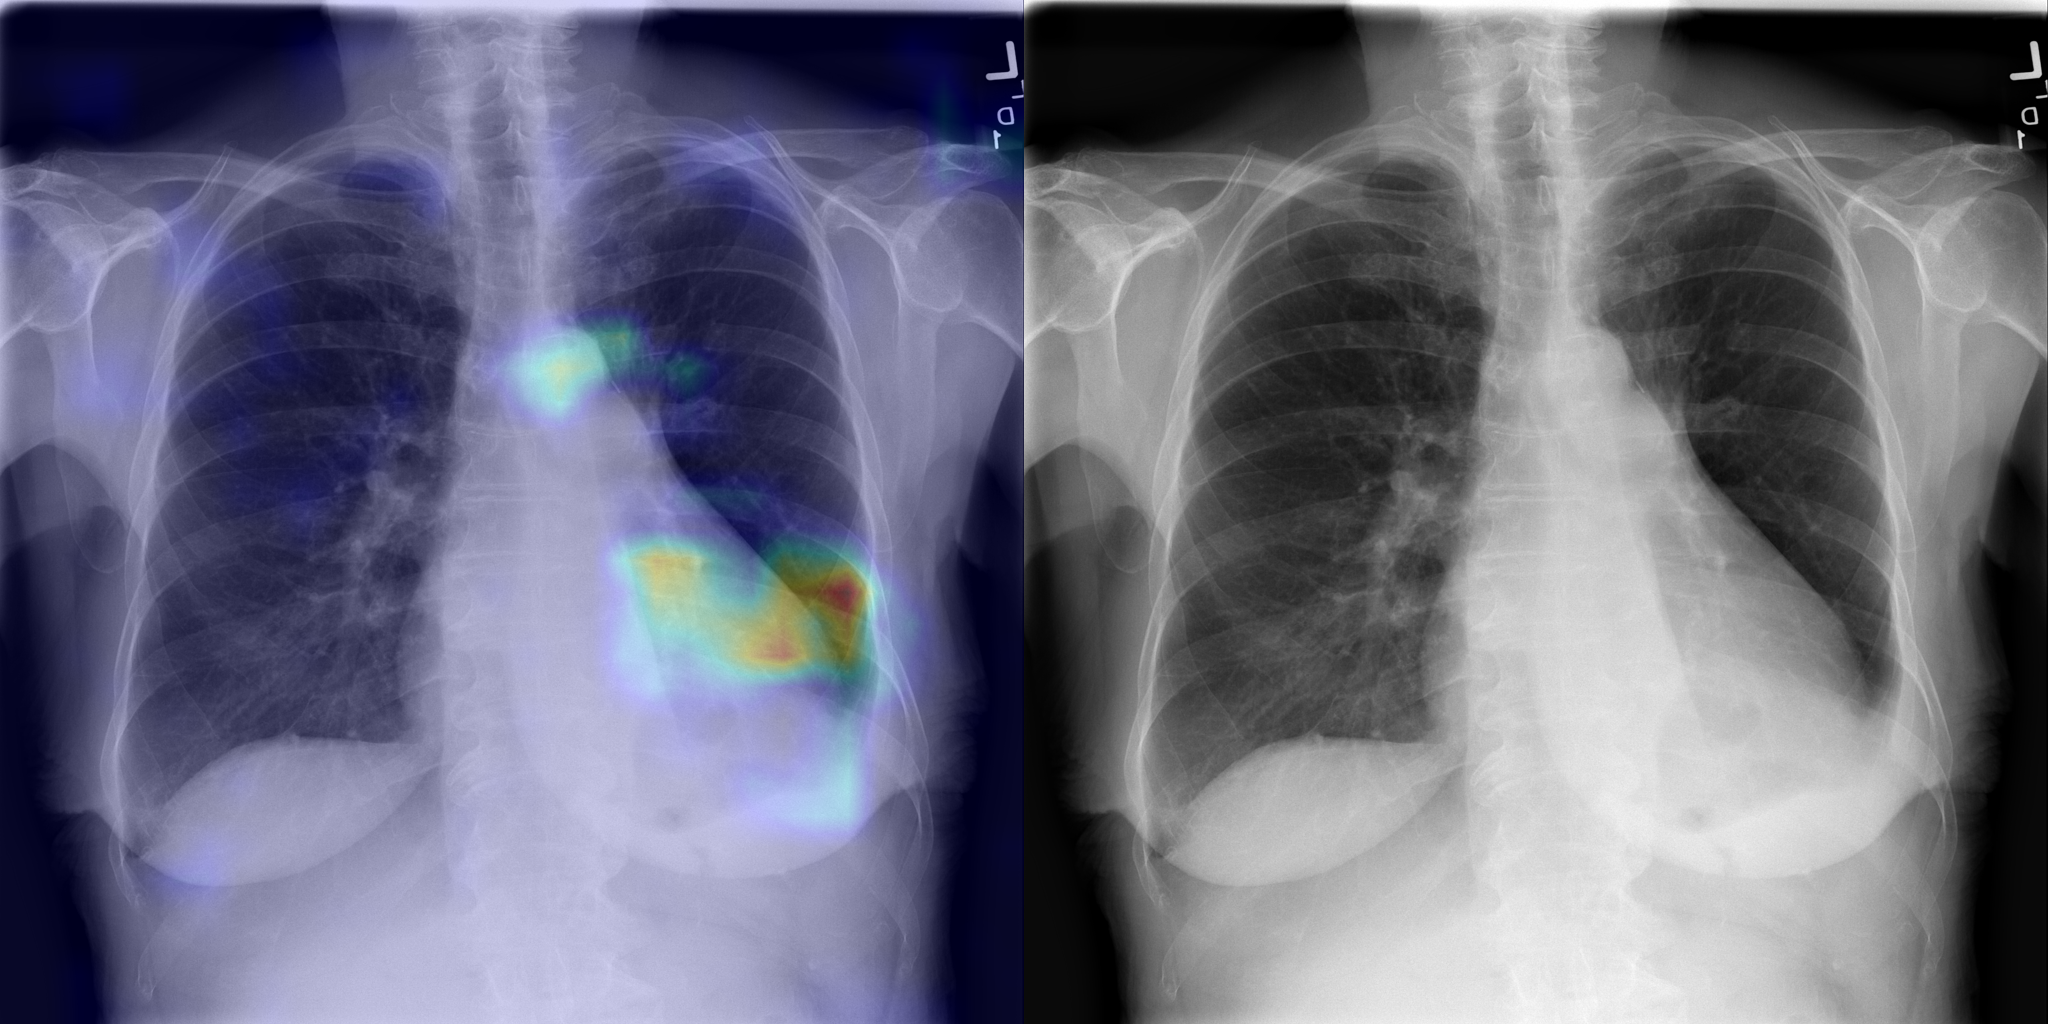
\includegraphics[width=1.0\textwidth]{Chapters/5. Conclusiones/img/Cardiomegaly/1_0_00000732_008.png}
    \end{subfigure}
    \begin{subfigure}{0.4\textwidth}
        \centering
        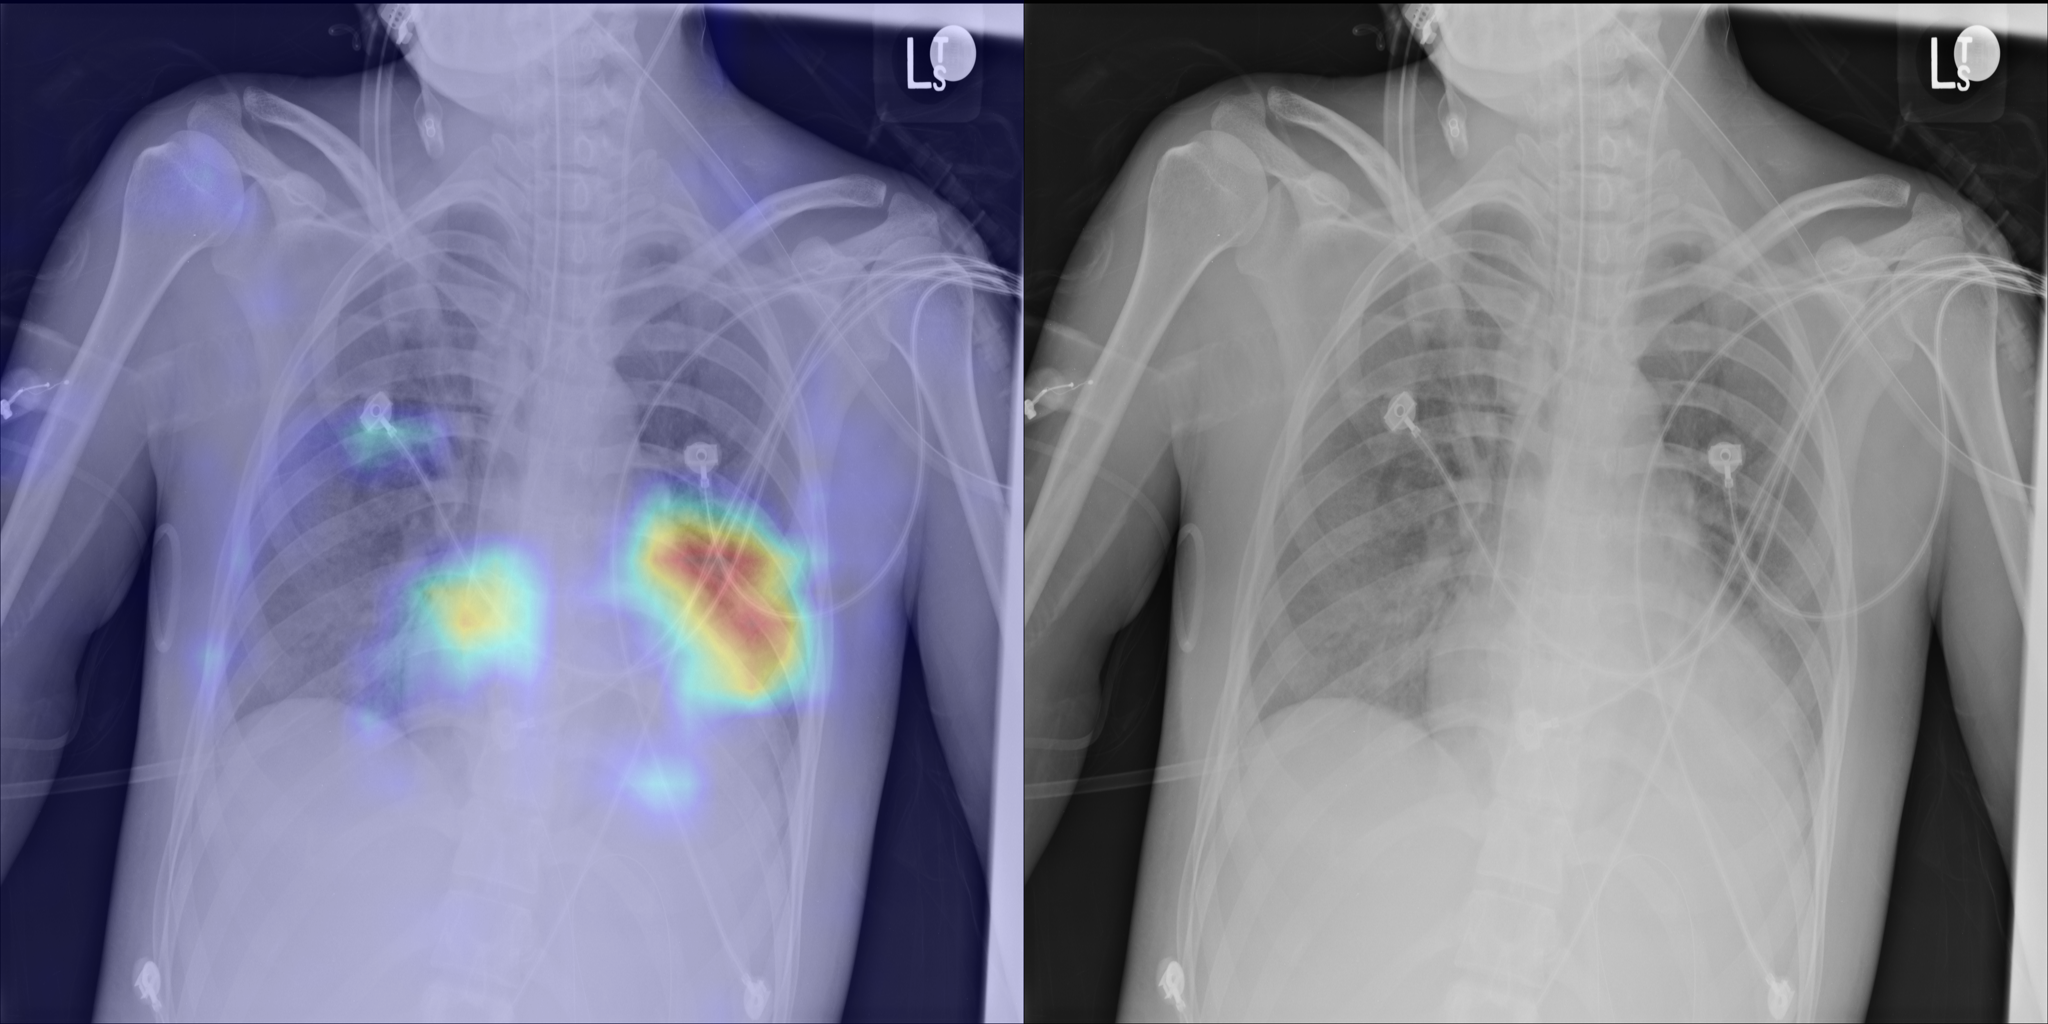
\includegraphics[width=1.0\textwidth]{Chapters/5. Conclusiones/img/Cardiomegaly/1_0_00001582_008.png}
    \end{subfigure}
    \begin{subfigure}{0.4\textwidth}
        \centering
        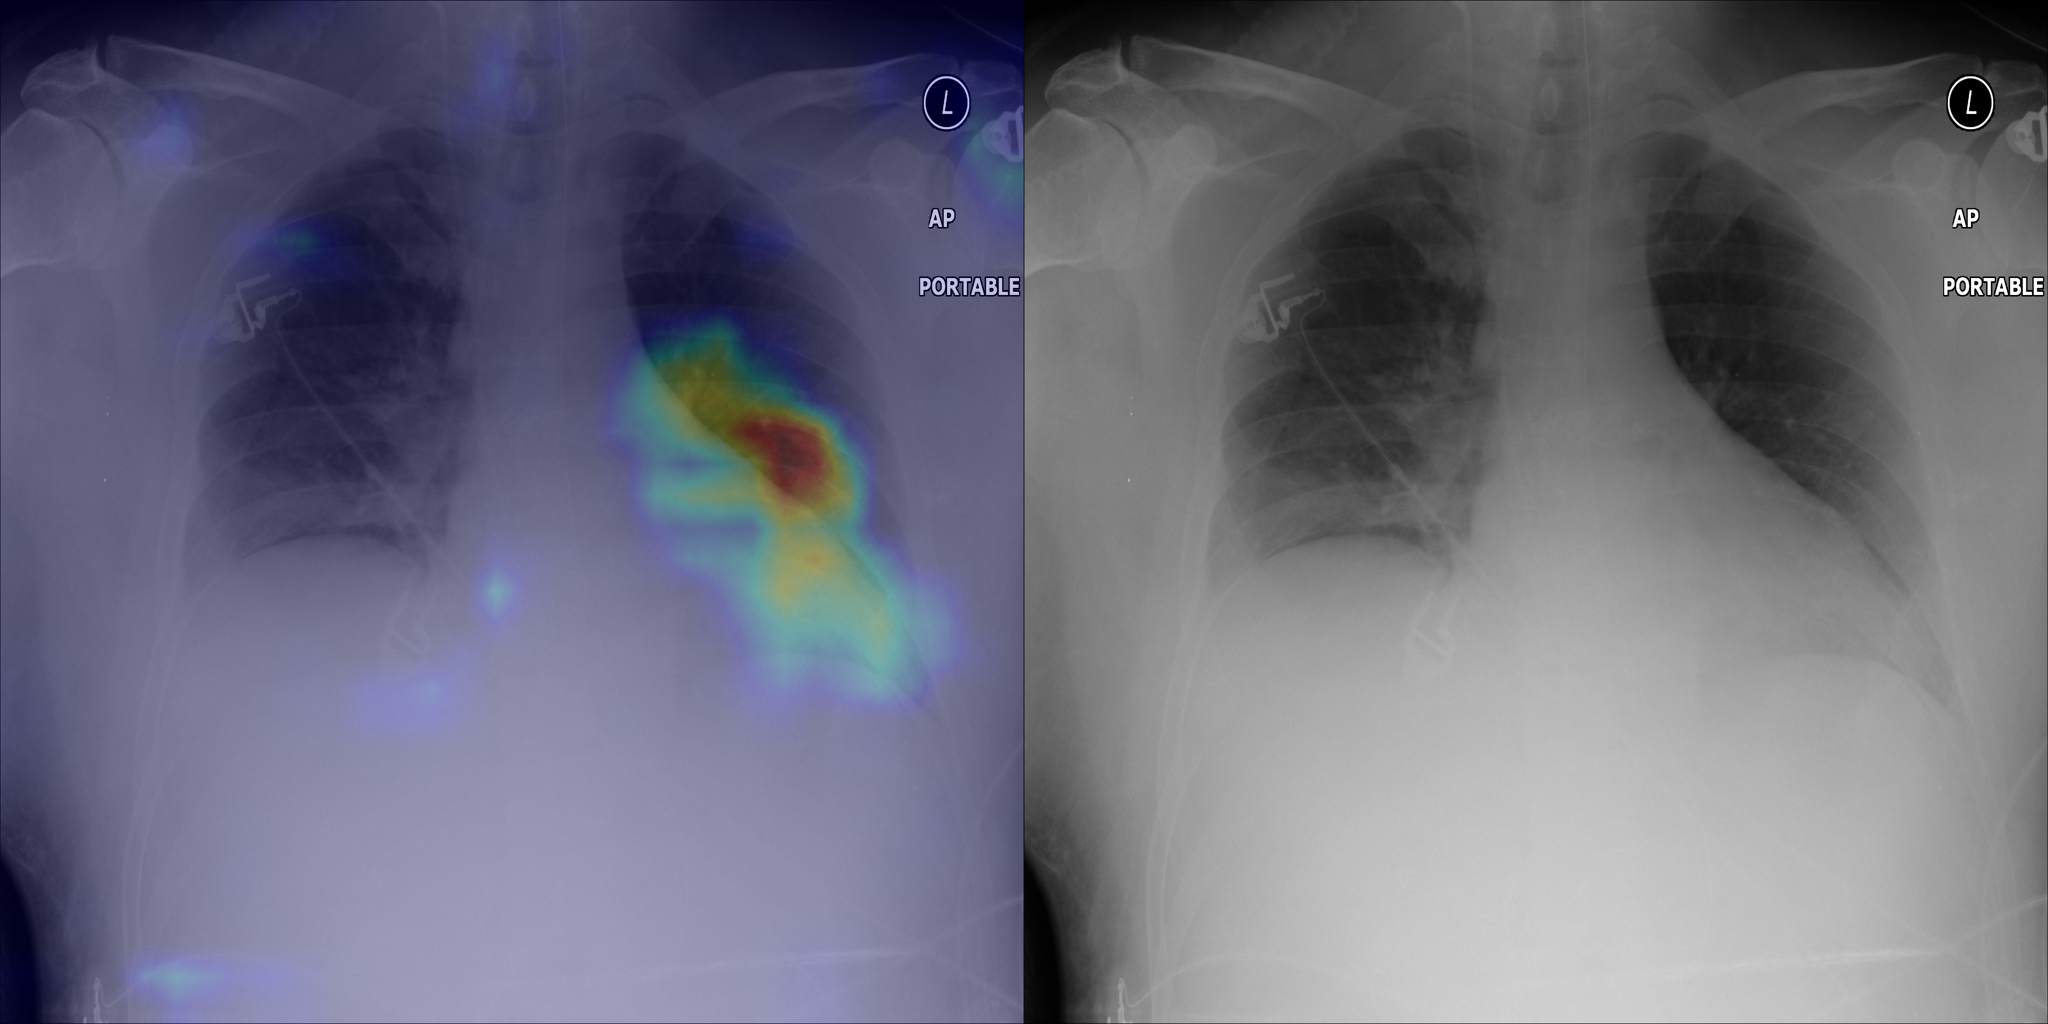
\includegraphics[width=1.0\textwidth]{Chapters/5. Conclusiones/img/Cardiomegaly/1_0_00002059_002.png}
    \end{subfigure}
    \begin{subfigure}{0.4\textwidth}
        \centering
        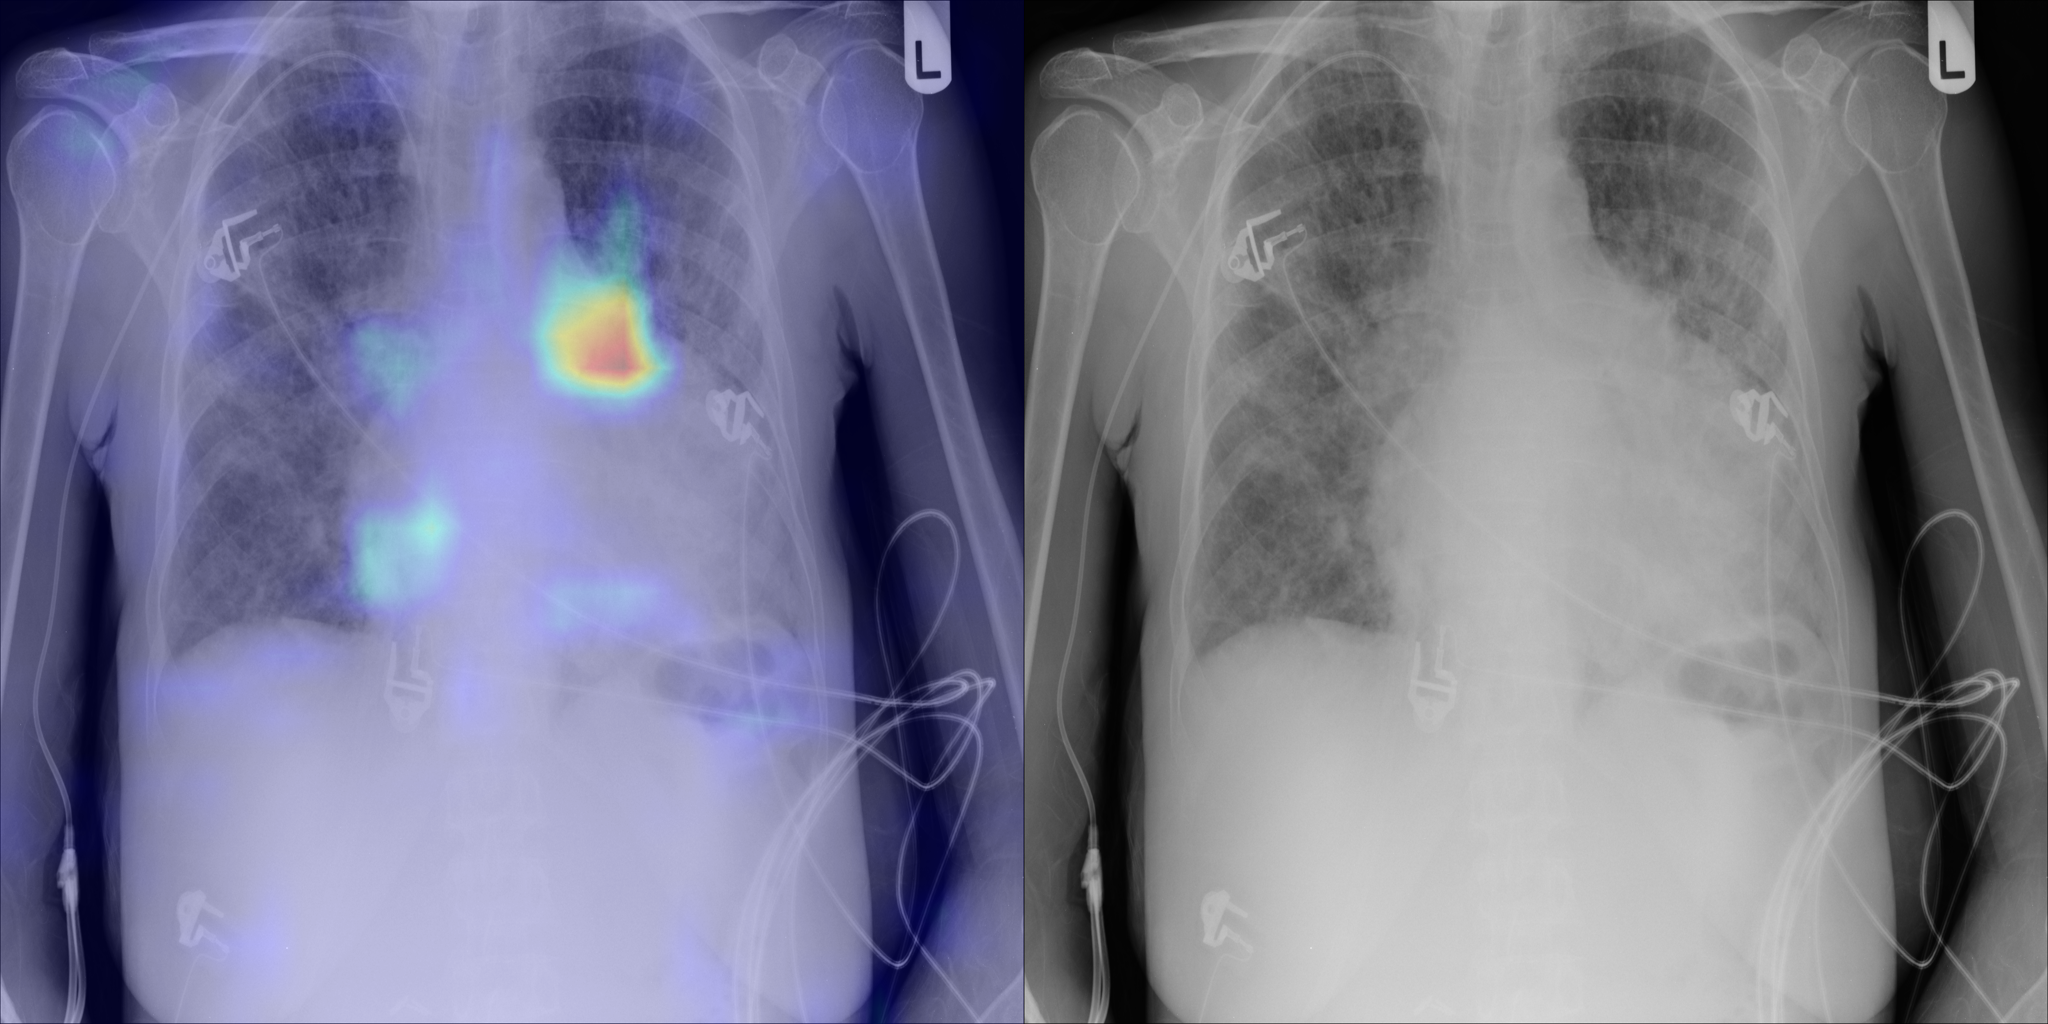
\includegraphics[width=1.0\textwidth]{Chapters/5. Conclusiones/img/Cardiomegaly/1_0_00004344_039.png}
    \end{subfigure}
    \begin{subfigure}{0.4\textwidth}
        \centering
        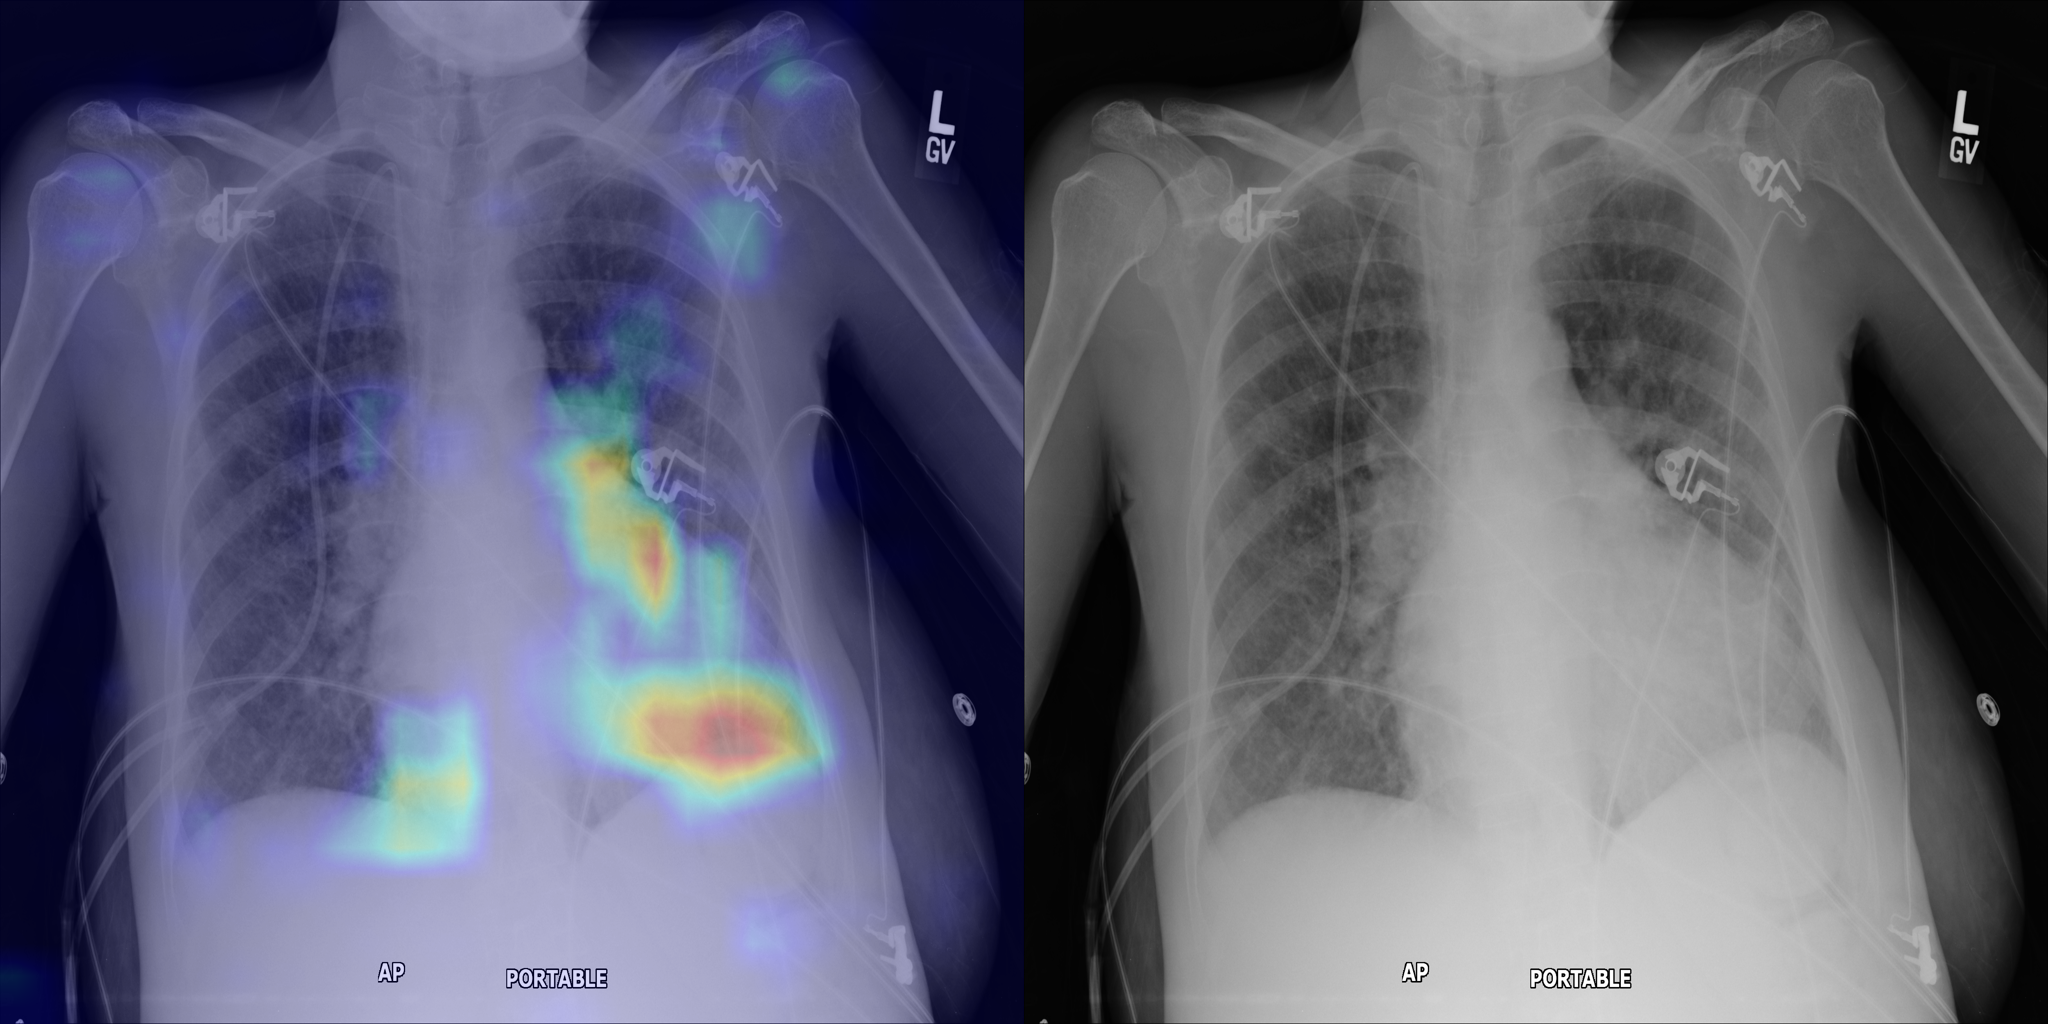
\includegraphics[width=1.0\textwidth]{Chapters/5. Conclusiones/img/Cardiomegaly/1_0_00004344_045.png}
    \end{subfigure}
    \begin{subfigure}{0.4\textwidth}
        \centering
        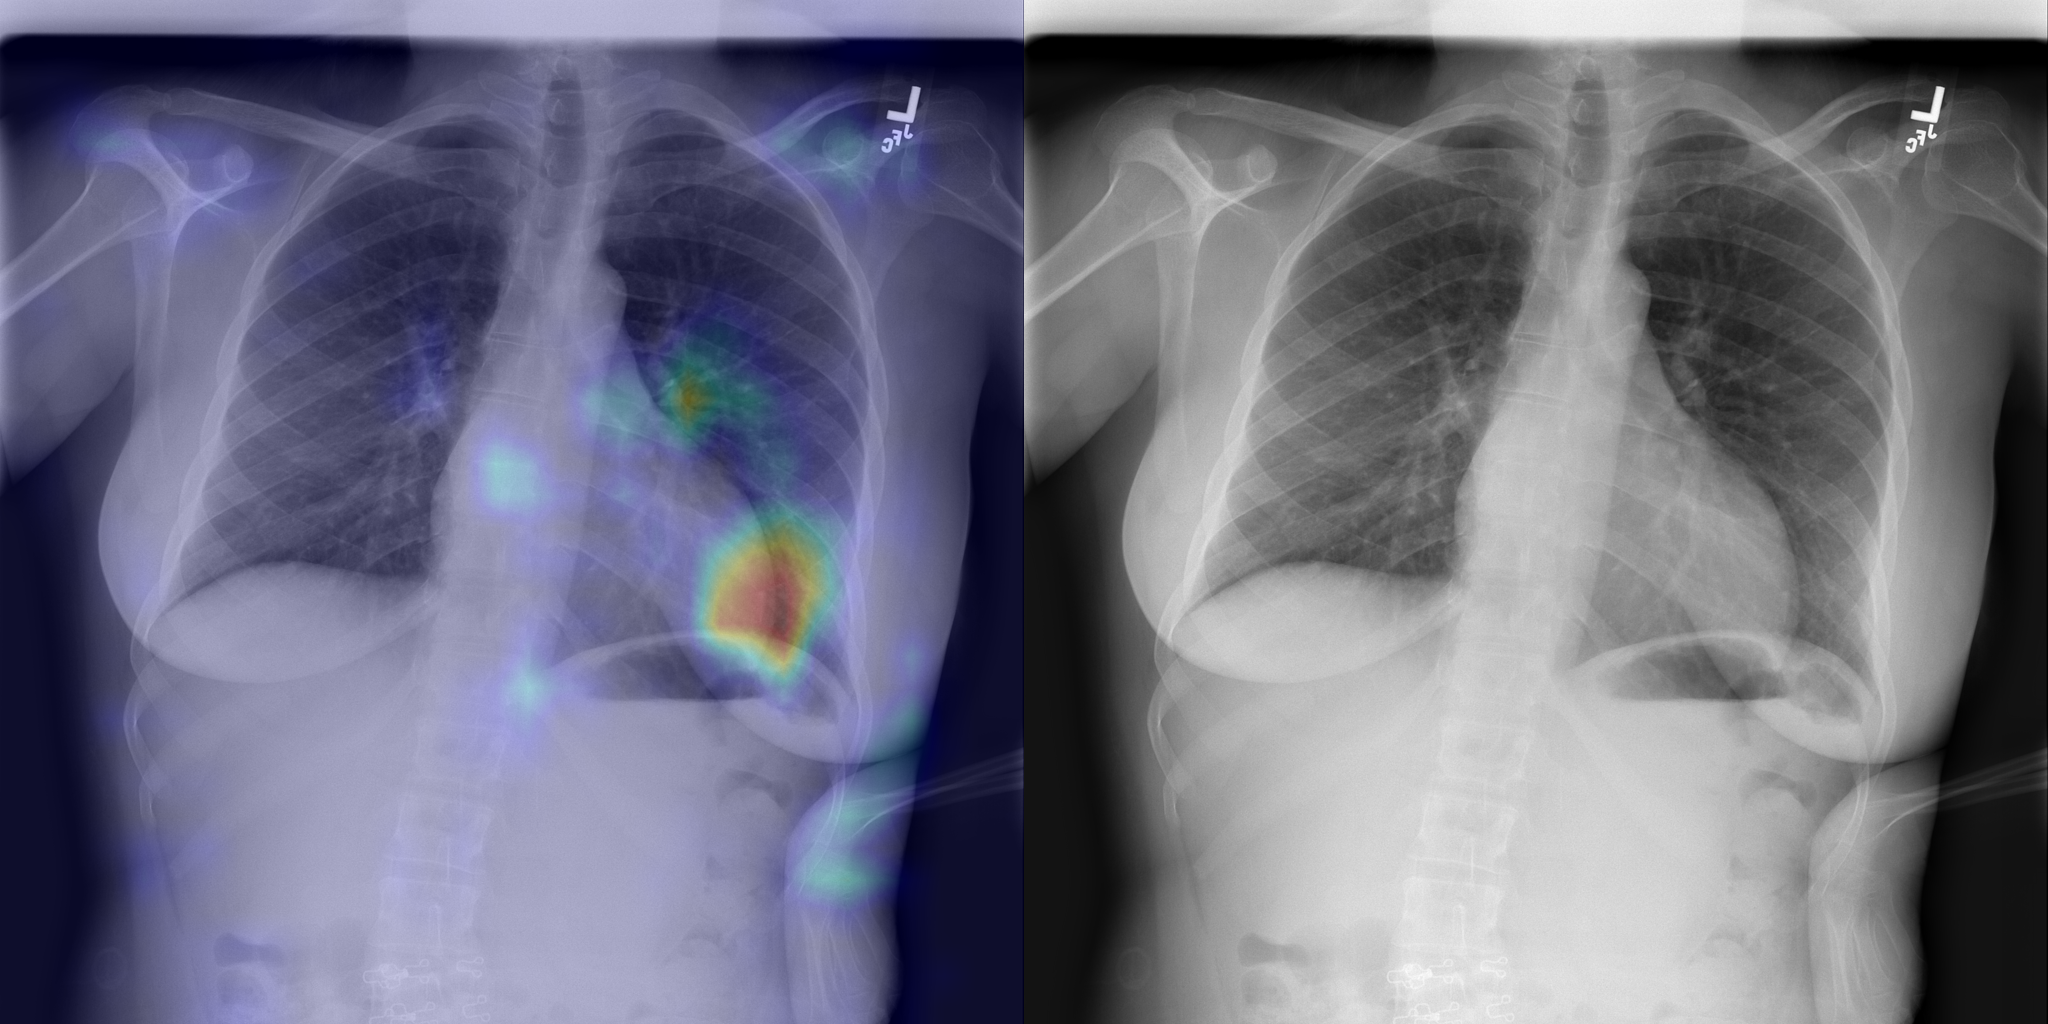
\includegraphics[width=1.0\textwidth]{Chapters/5. Conclusiones/img/Cardiomegaly/1_0_00004526_017.png}
    \end{subfigure}
    \begin{subfigure}{0.4\textwidth}
        \centering
        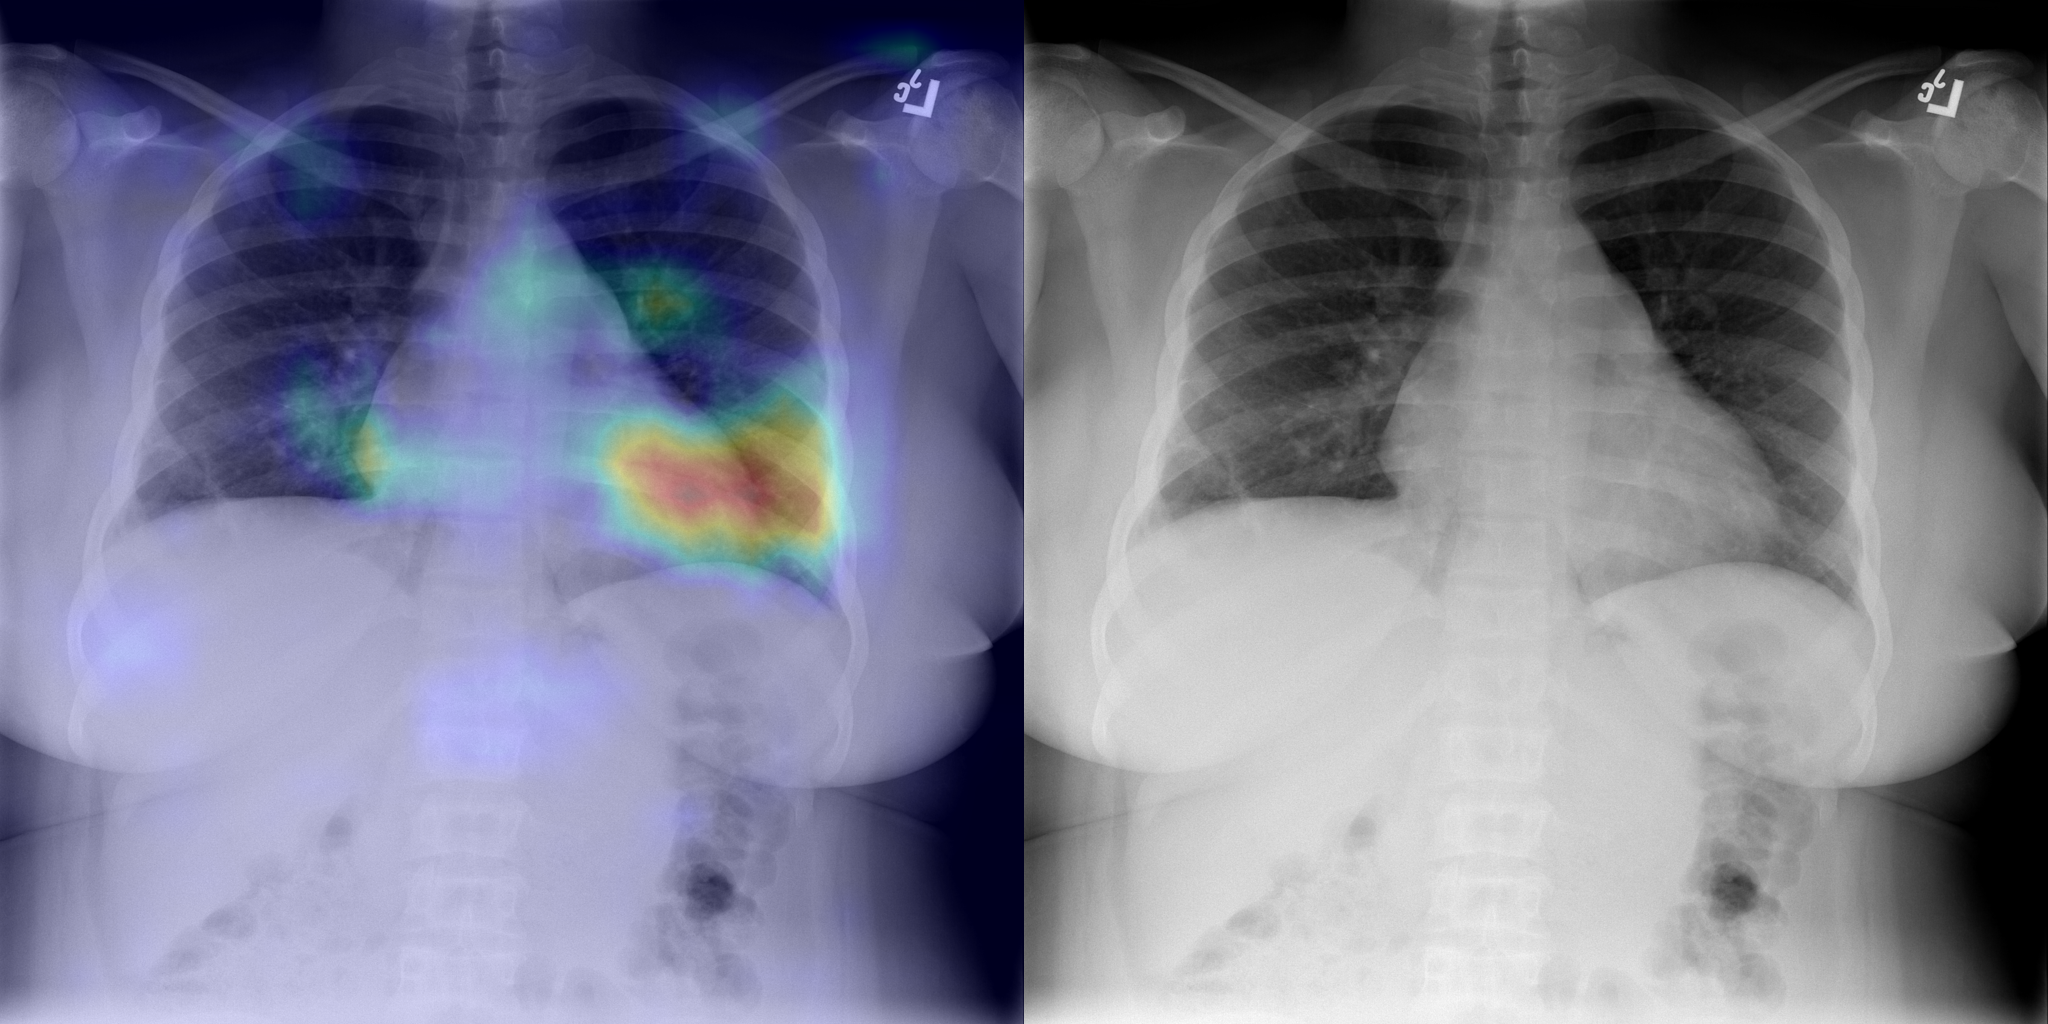
\includegraphics[width=1.0\textwidth]{Chapters/5. Conclusiones/img/Cardiomegaly/1_1_00014706_010.png}
    \end{subfigure}
    \begin{subfigure}{0.4\textwidth}
        \centering
        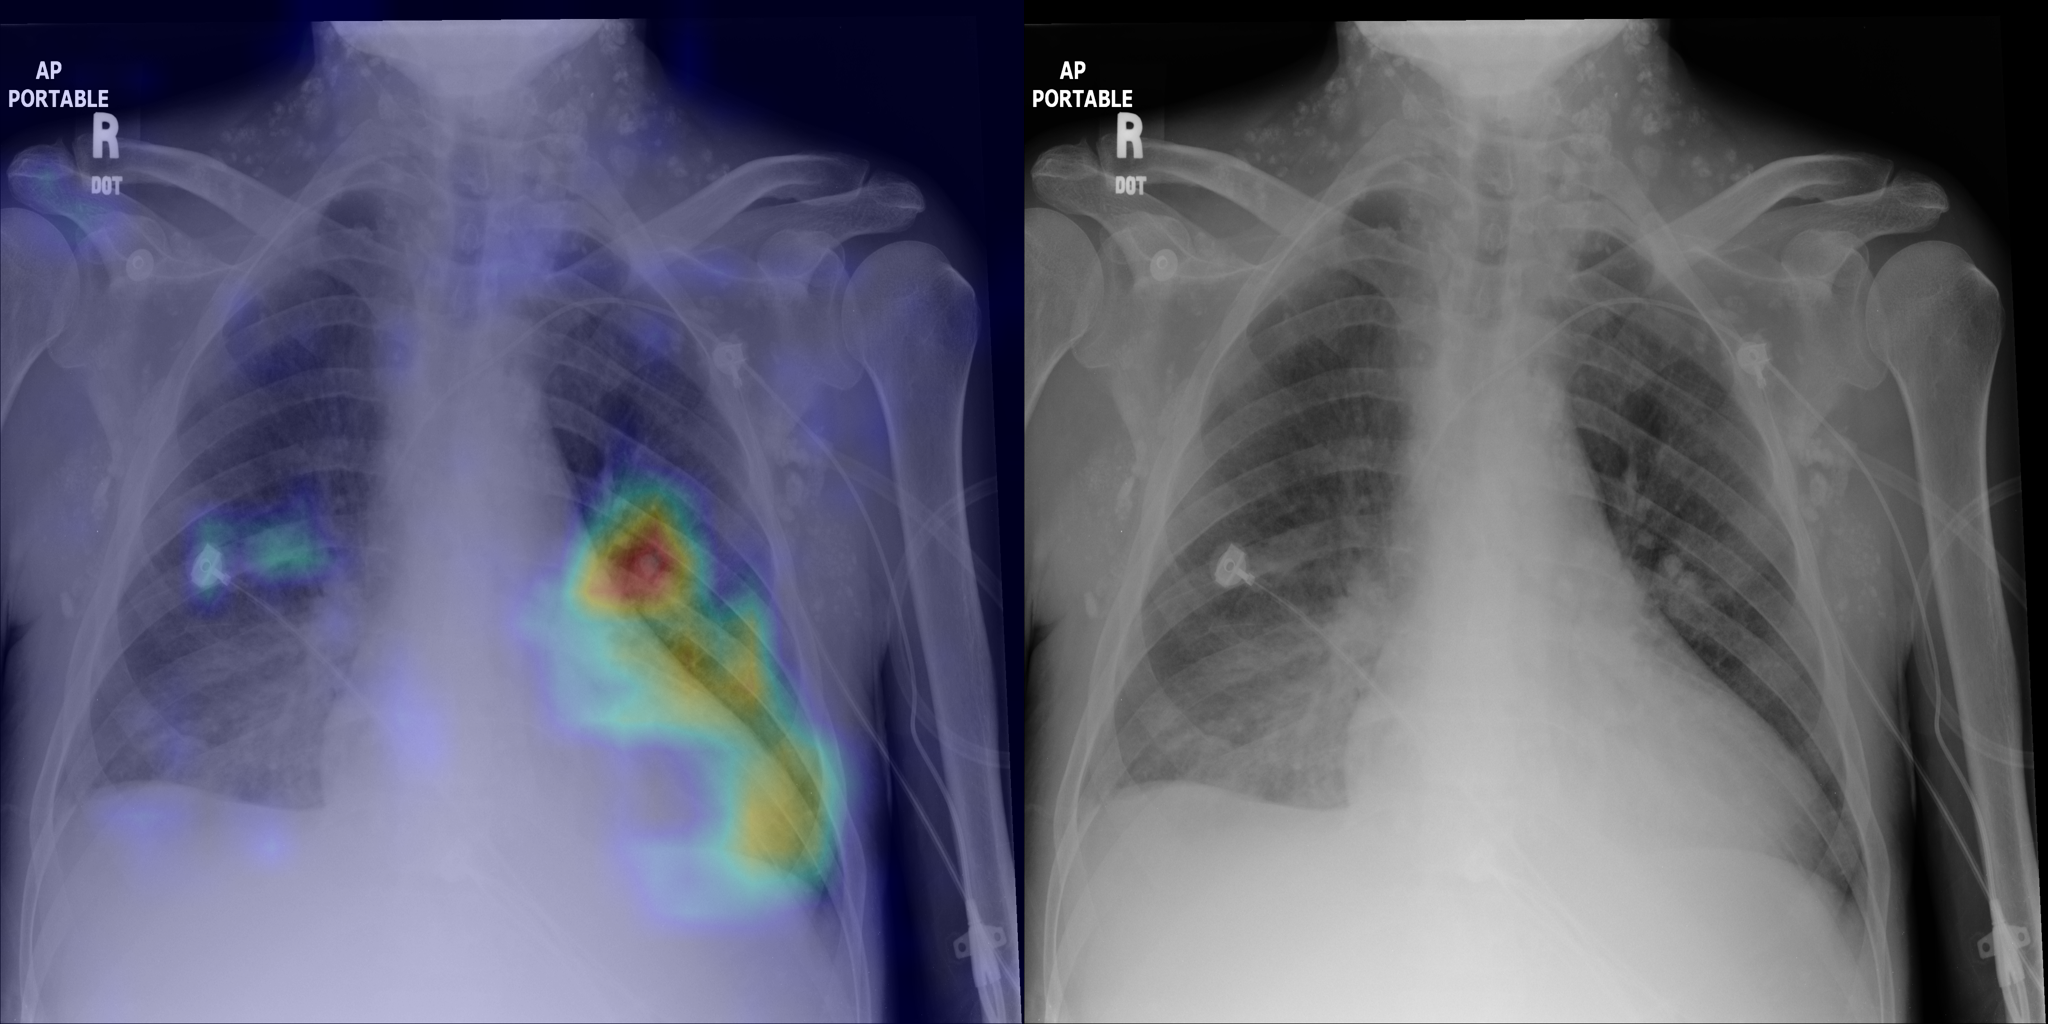
\includegraphics[width=1.0\textwidth]{Chapters/5. Conclusiones/img/Cardiomegaly/1_1_00016291_042.png}
    \end{subfigure}

    \caption[short]{Cardiomegalia. Radiografías detectadas con la patología de cardiomegalia por los
                    radiólogos. A la izquierda de cada imagen el GradCam correspondiente a la detección
                    de la patología como positivo por el modelo CNN.}
\end{figure}

\begin{figure}[b]
    \centering
    \begin{subfigure}{0.4\textwidth}
        \centering
        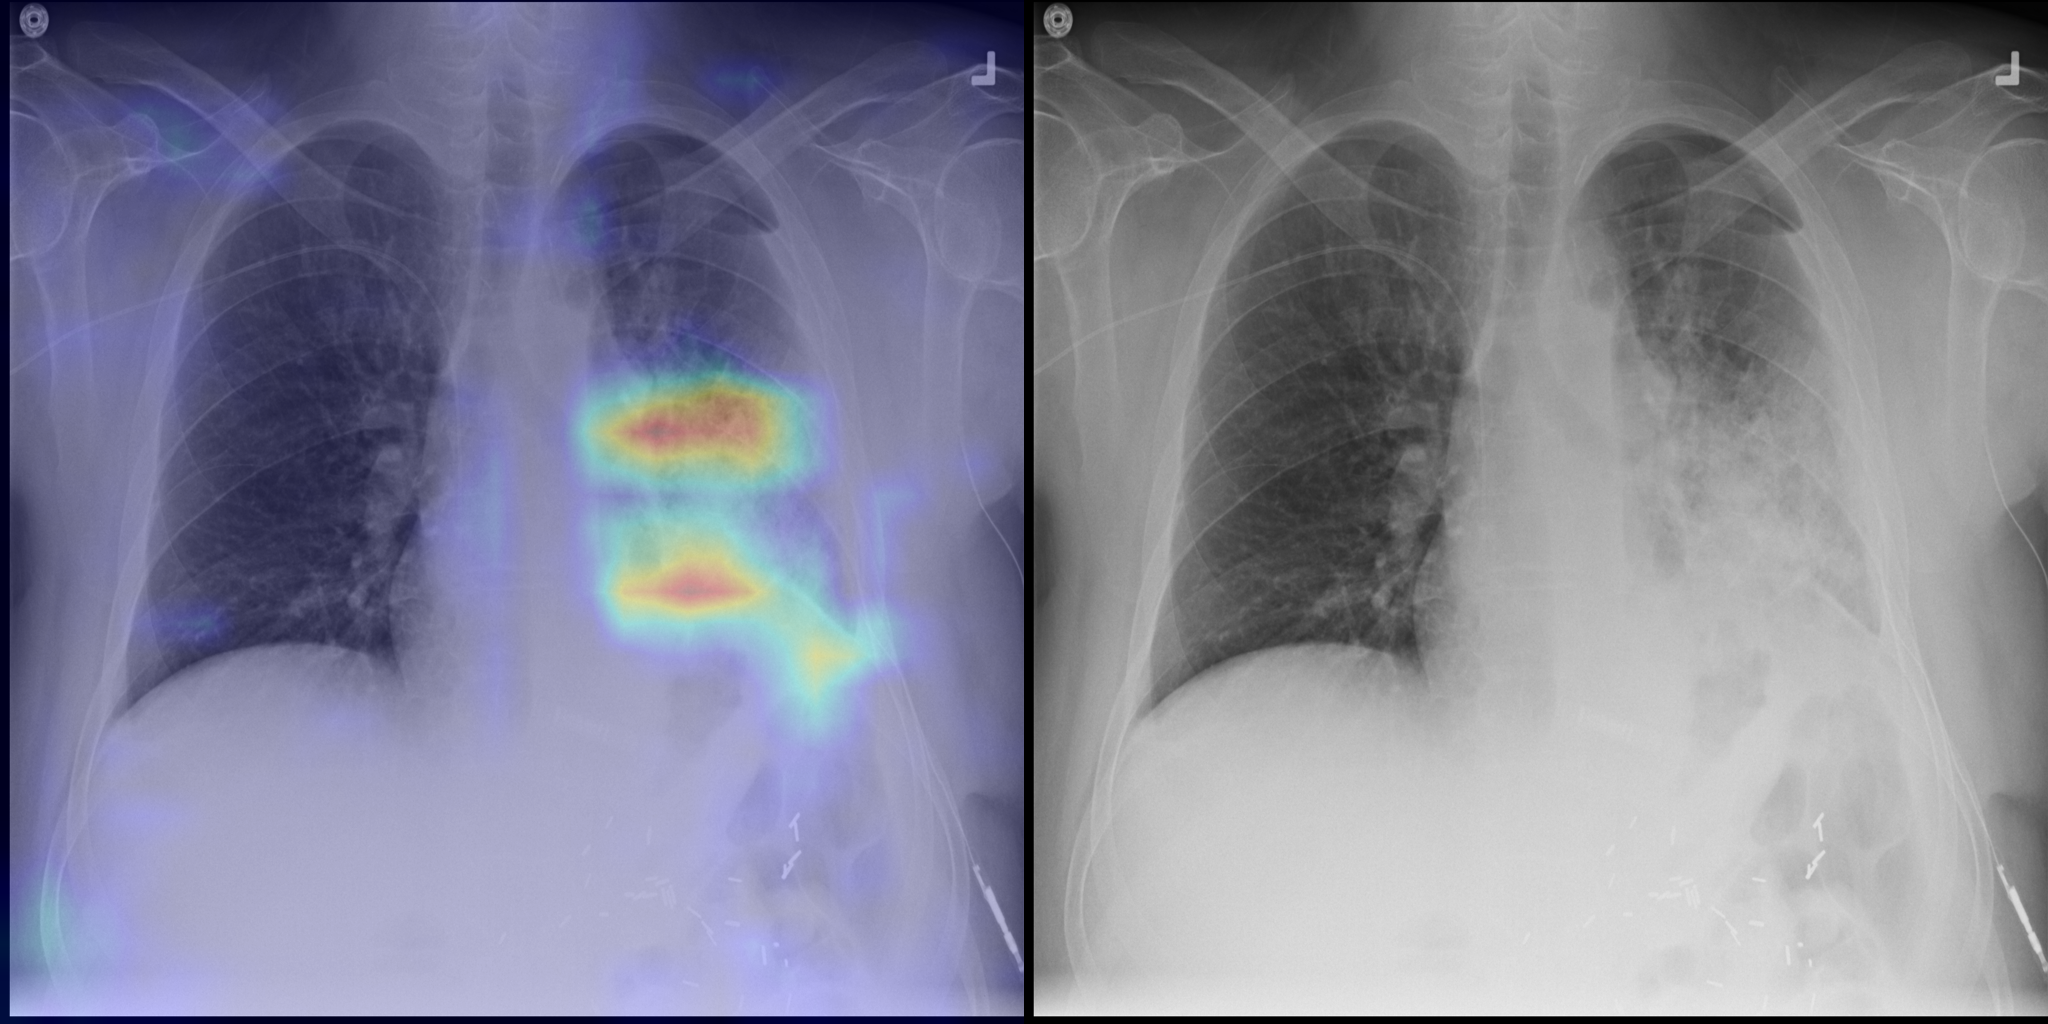
\includegraphics[width=1.0\textwidth]{Chapters/5. Conclusiones/img/Consolidation/1_1_00000246_014.png}
    \end{subfigure}
    \begin{subfigure}{0.4\textwidth}
        \centering
        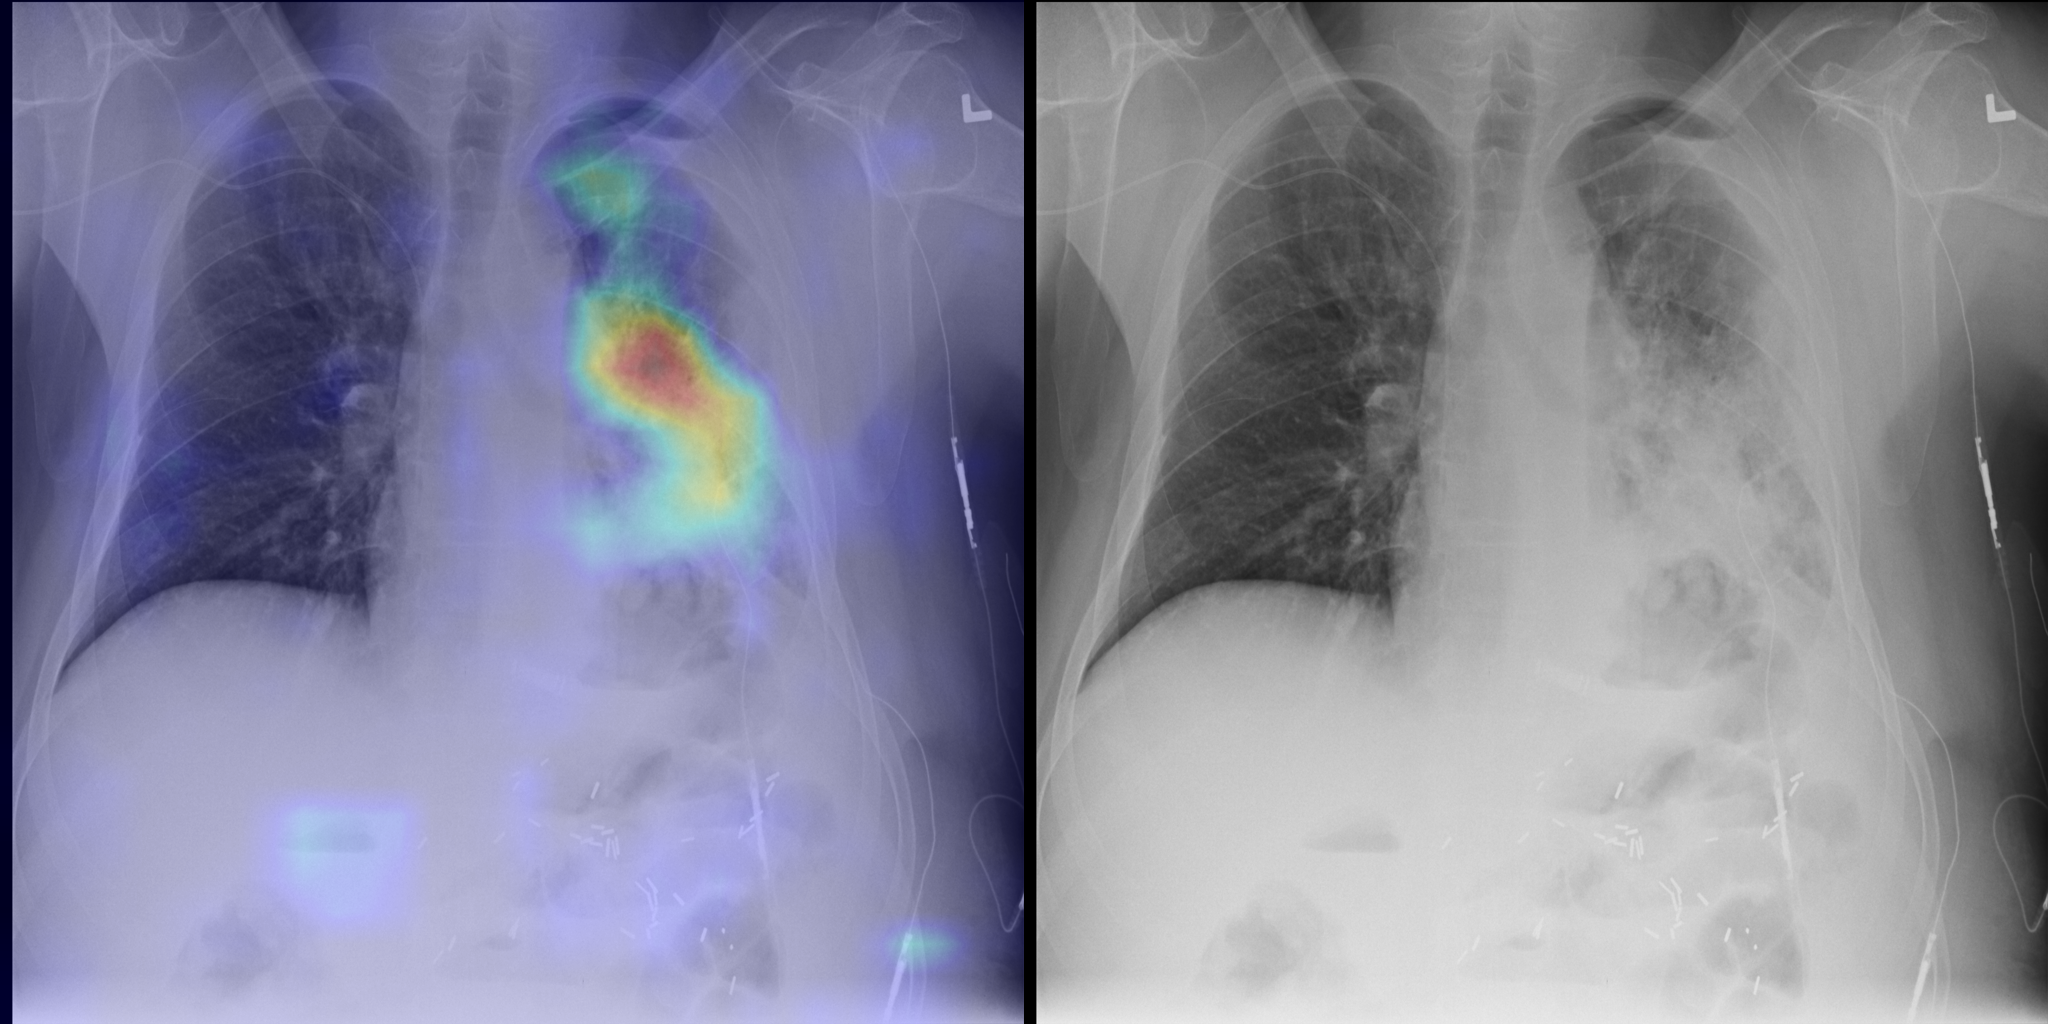
\includegraphics[width=1.0\textwidth]{Chapters/5. Conclusiones/img/Consolidation/1_1_00000246_016.png}
    \end{subfigure}
    \begin{subfigure}{0.4\textwidth}
        \centering
        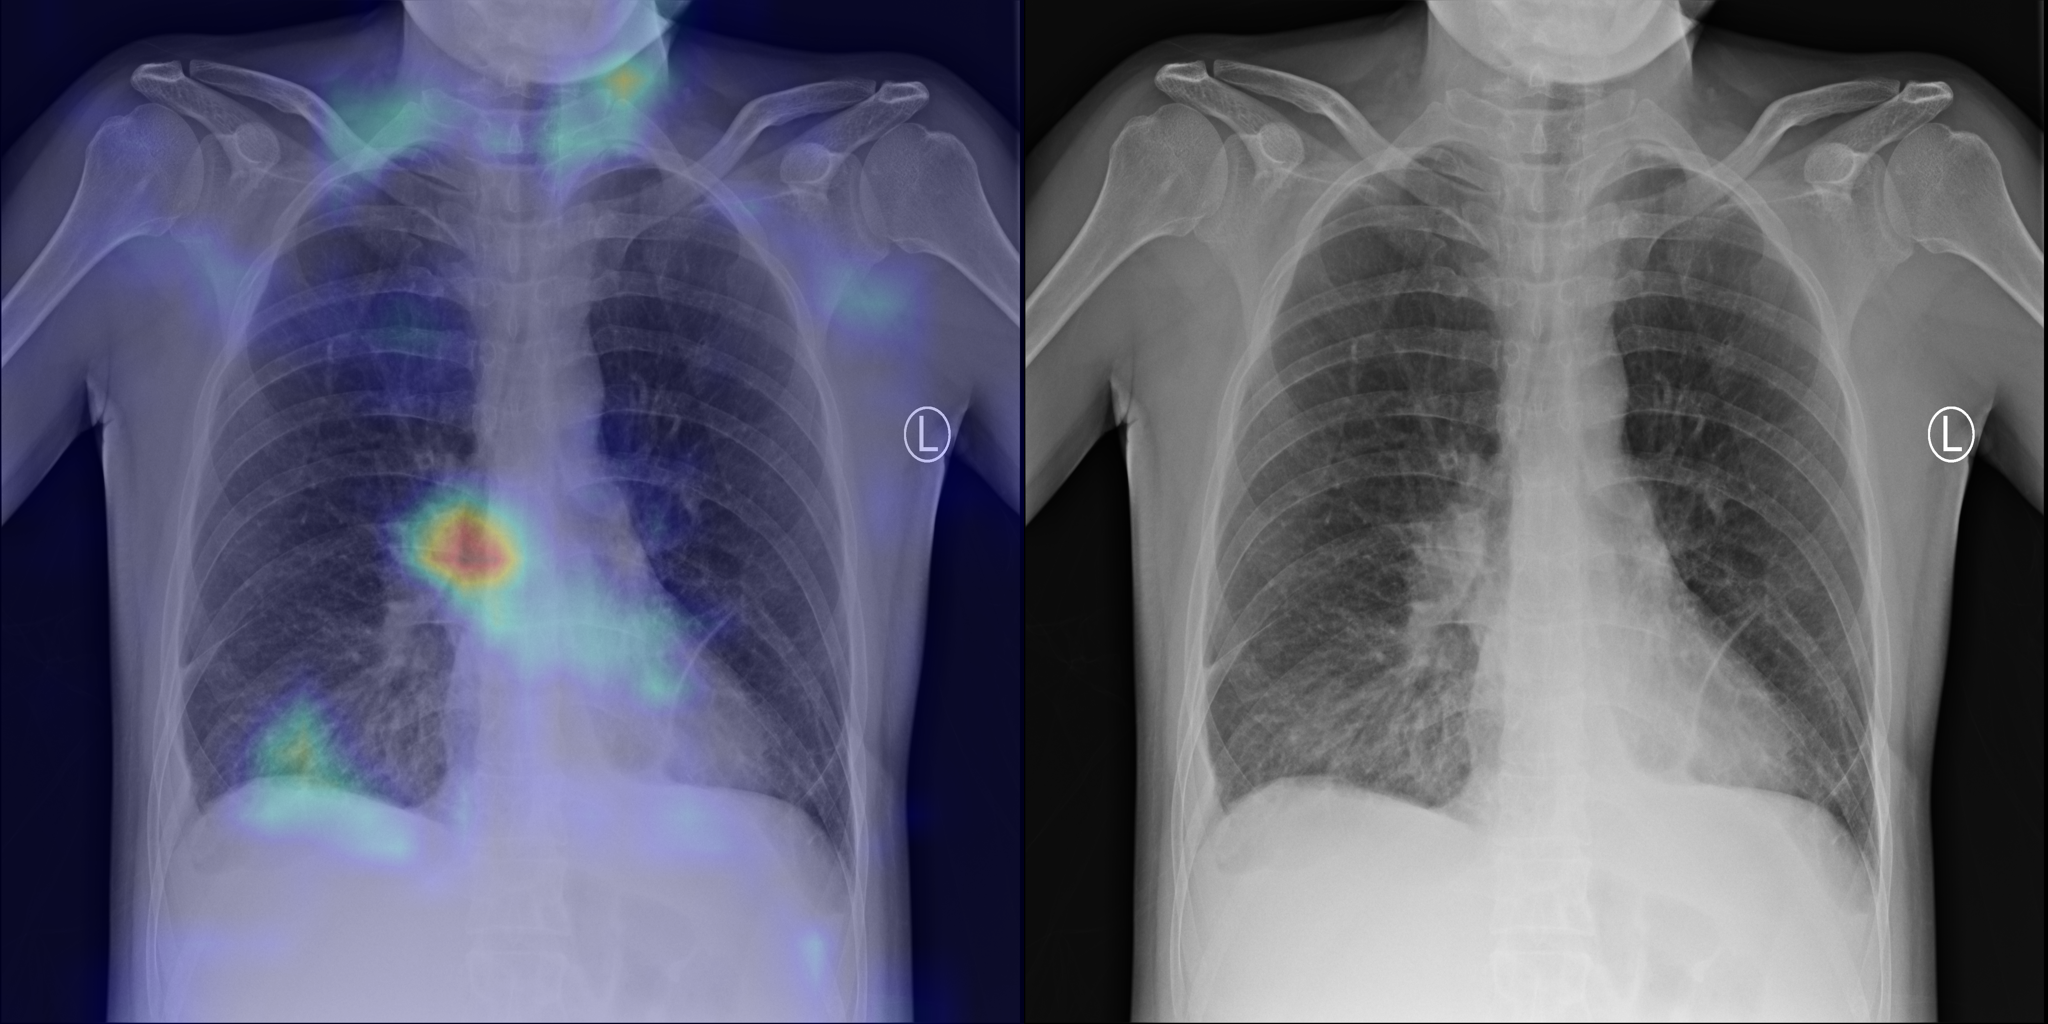
\includegraphics[width=1.0\textwidth]{Chapters/5. Conclusiones/img/Consolidation/1_1_00000344_000.png}
    \end{subfigure}
    \begin{subfigure}{0.4\textwidth}
        \centering
        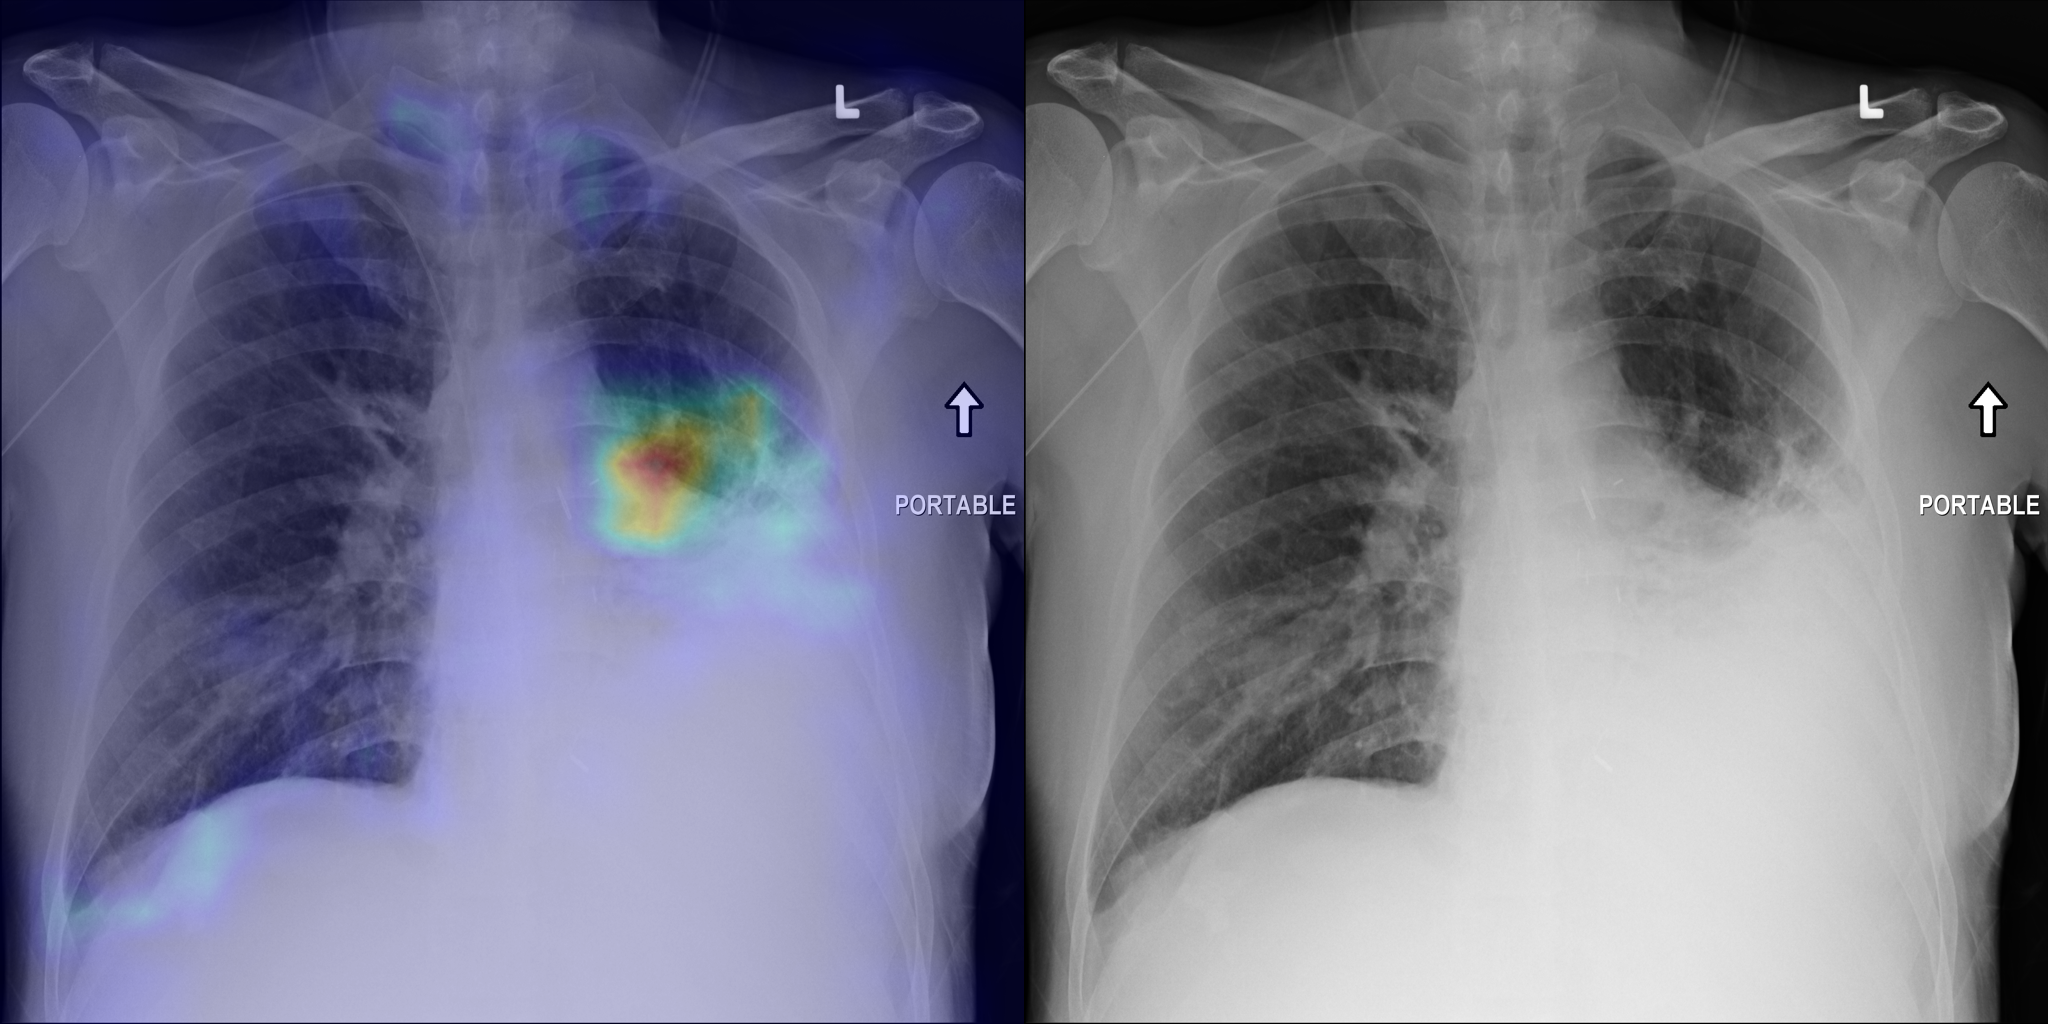
\includegraphics[width=1.0\textwidth]{Chapters/5. Conclusiones/img/Consolidation/1_1_00000467_002.png}
    \end{subfigure}
    \begin{subfigure}{0.4\textwidth}
        \centering
        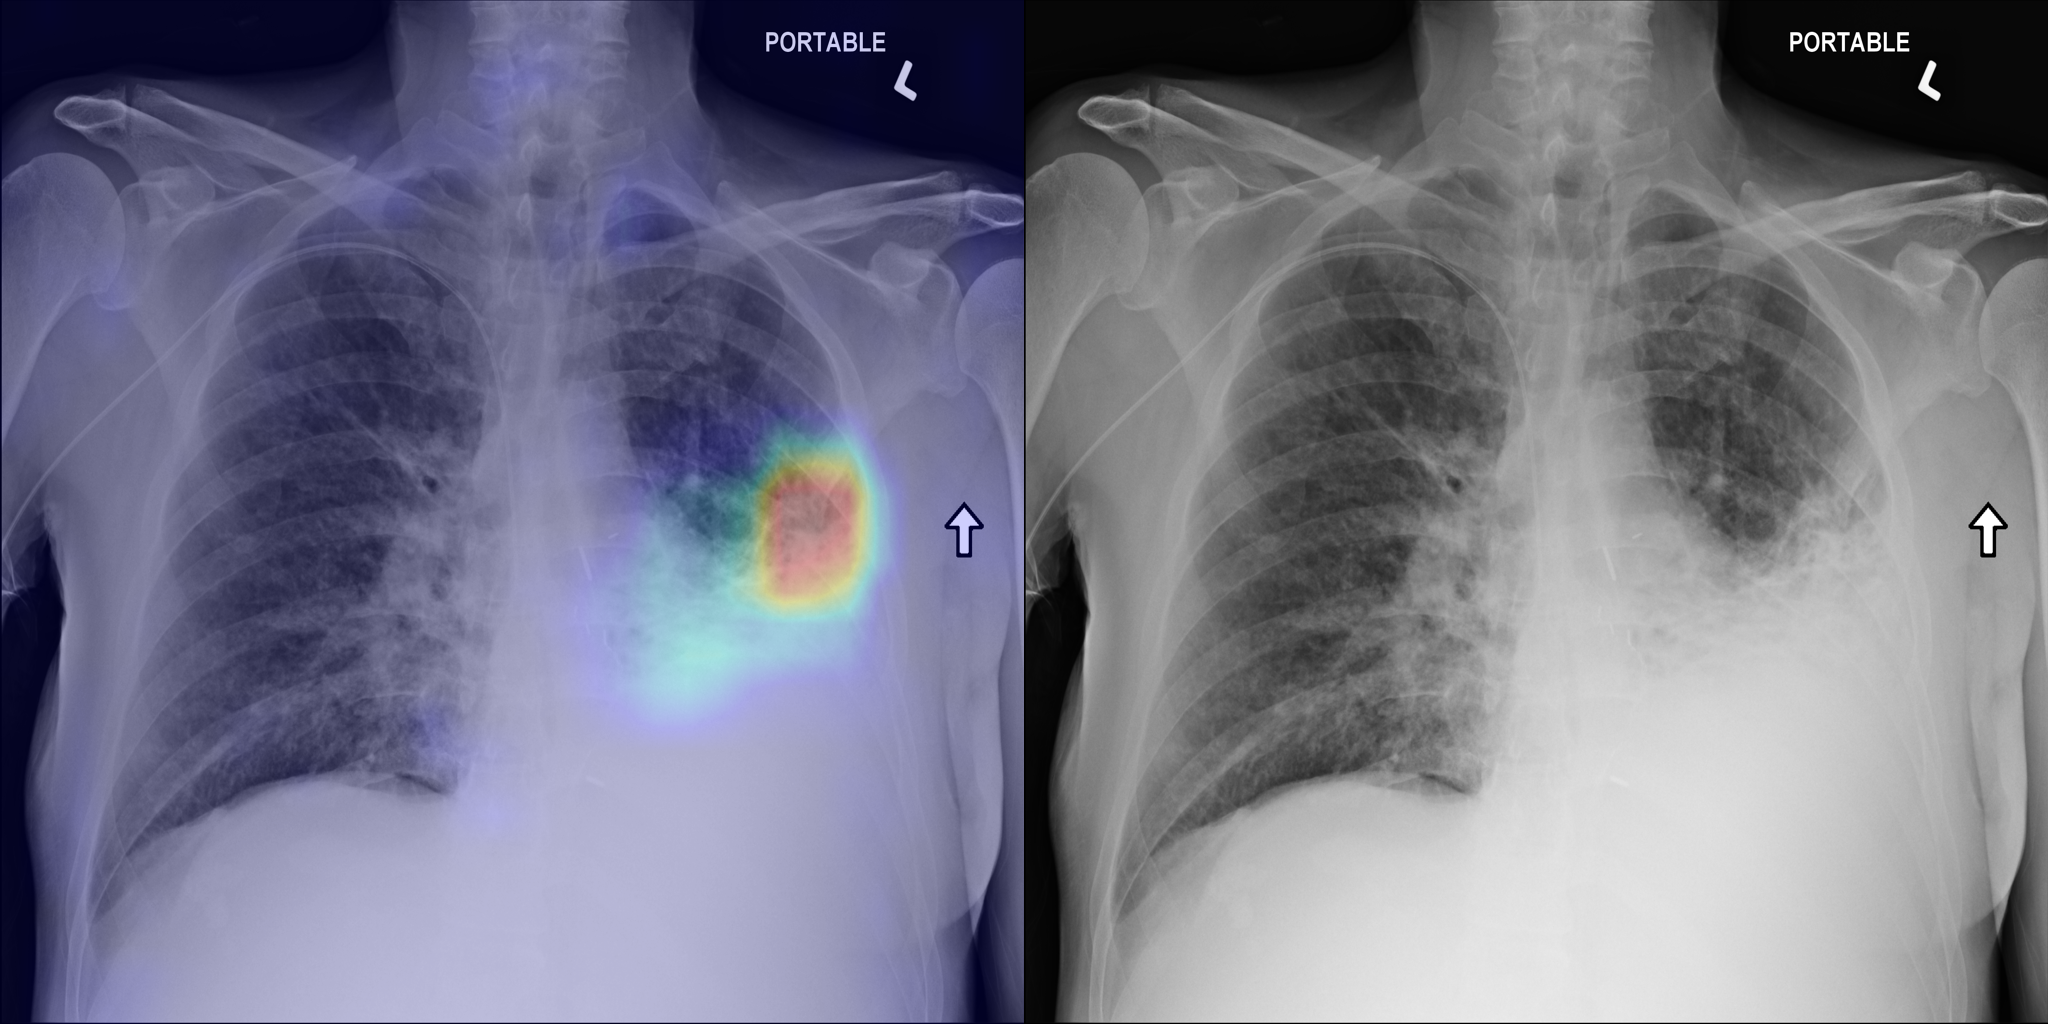
\includegraphics[width=1.0\textwidth]{Chapters/5. Conclusiones/img/Consolidation/1_1_00000467_003.png}
    \end{subfigure}
    \begin{subfigure}{0.4\textwidth}
        \centering
        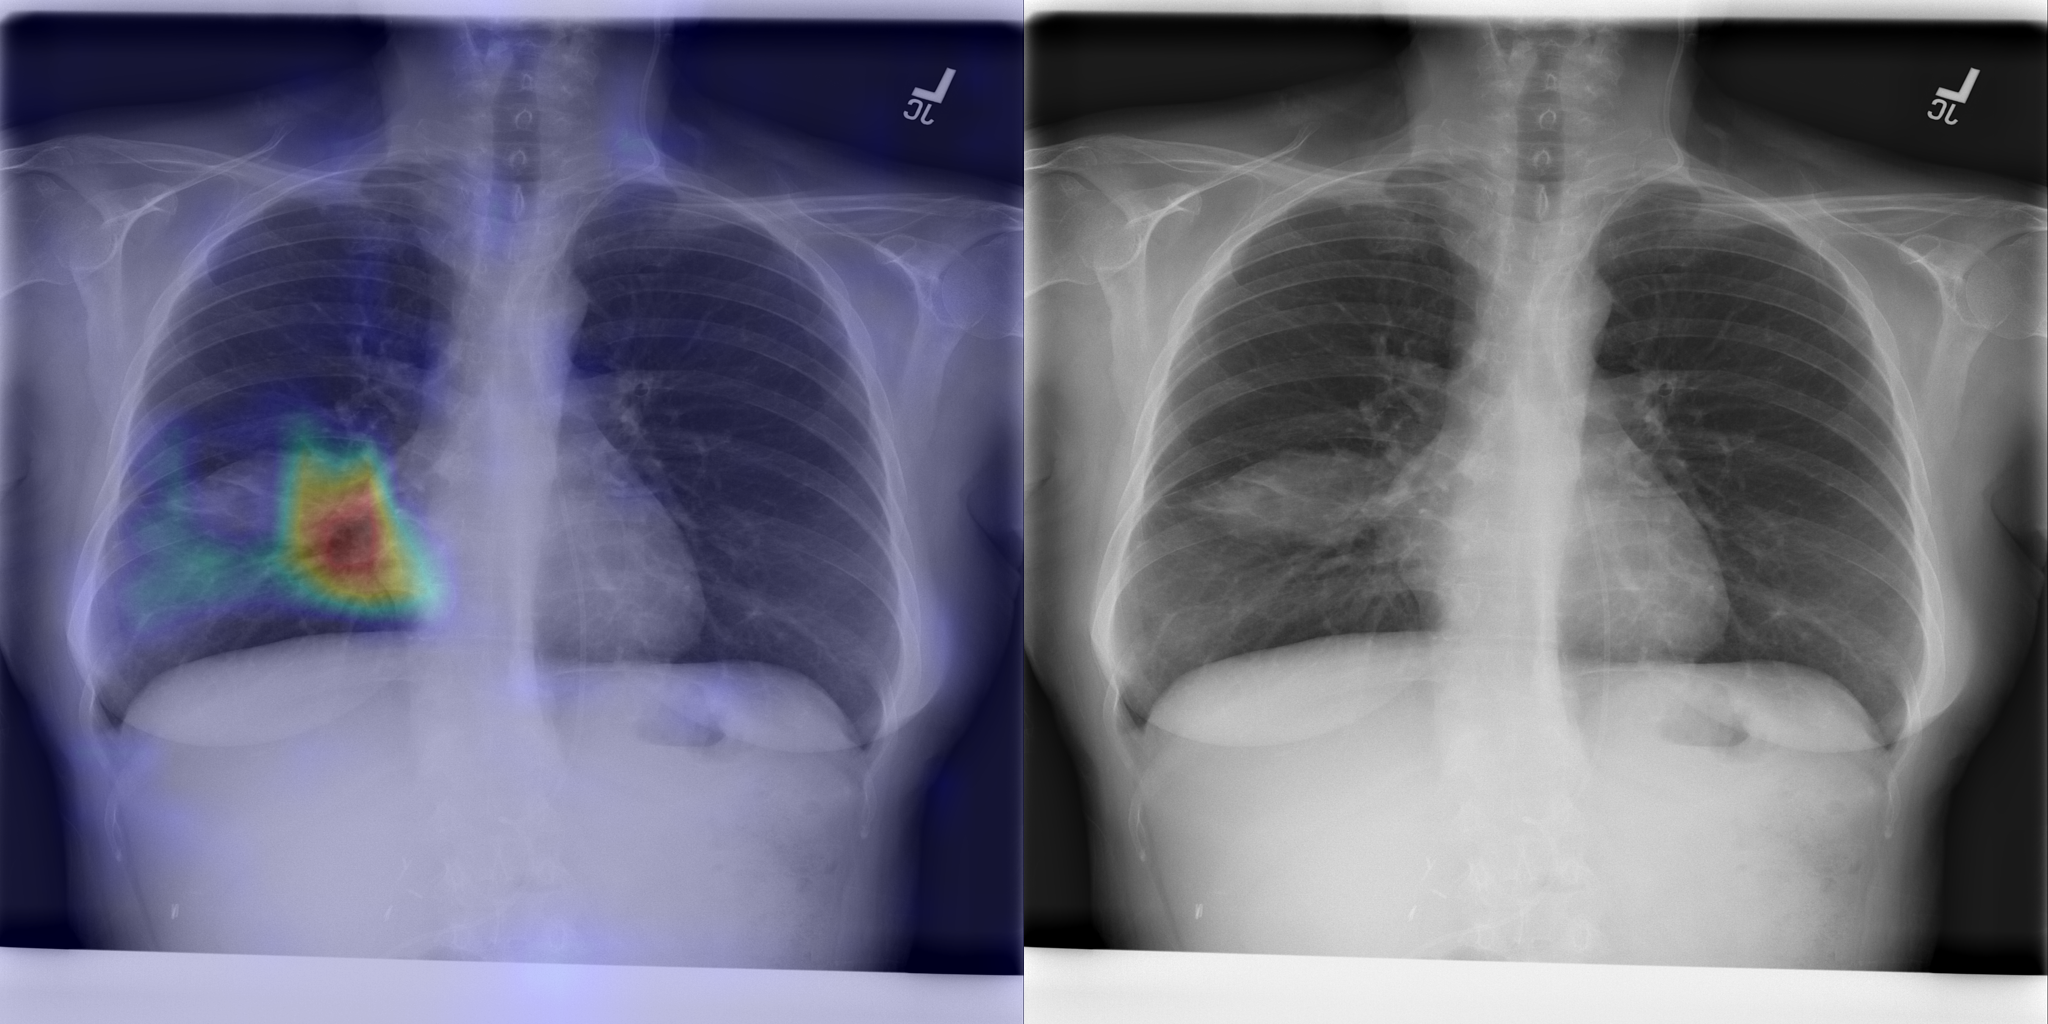
\includegraphics[width=1.0\textwidth]{Chapters/5. Conclusiones/img/Consolidation/1_1_00000618_008.png}
    \end{subfigure}
    \begin{subfigure}{0.4\textwidth}
        \centering
        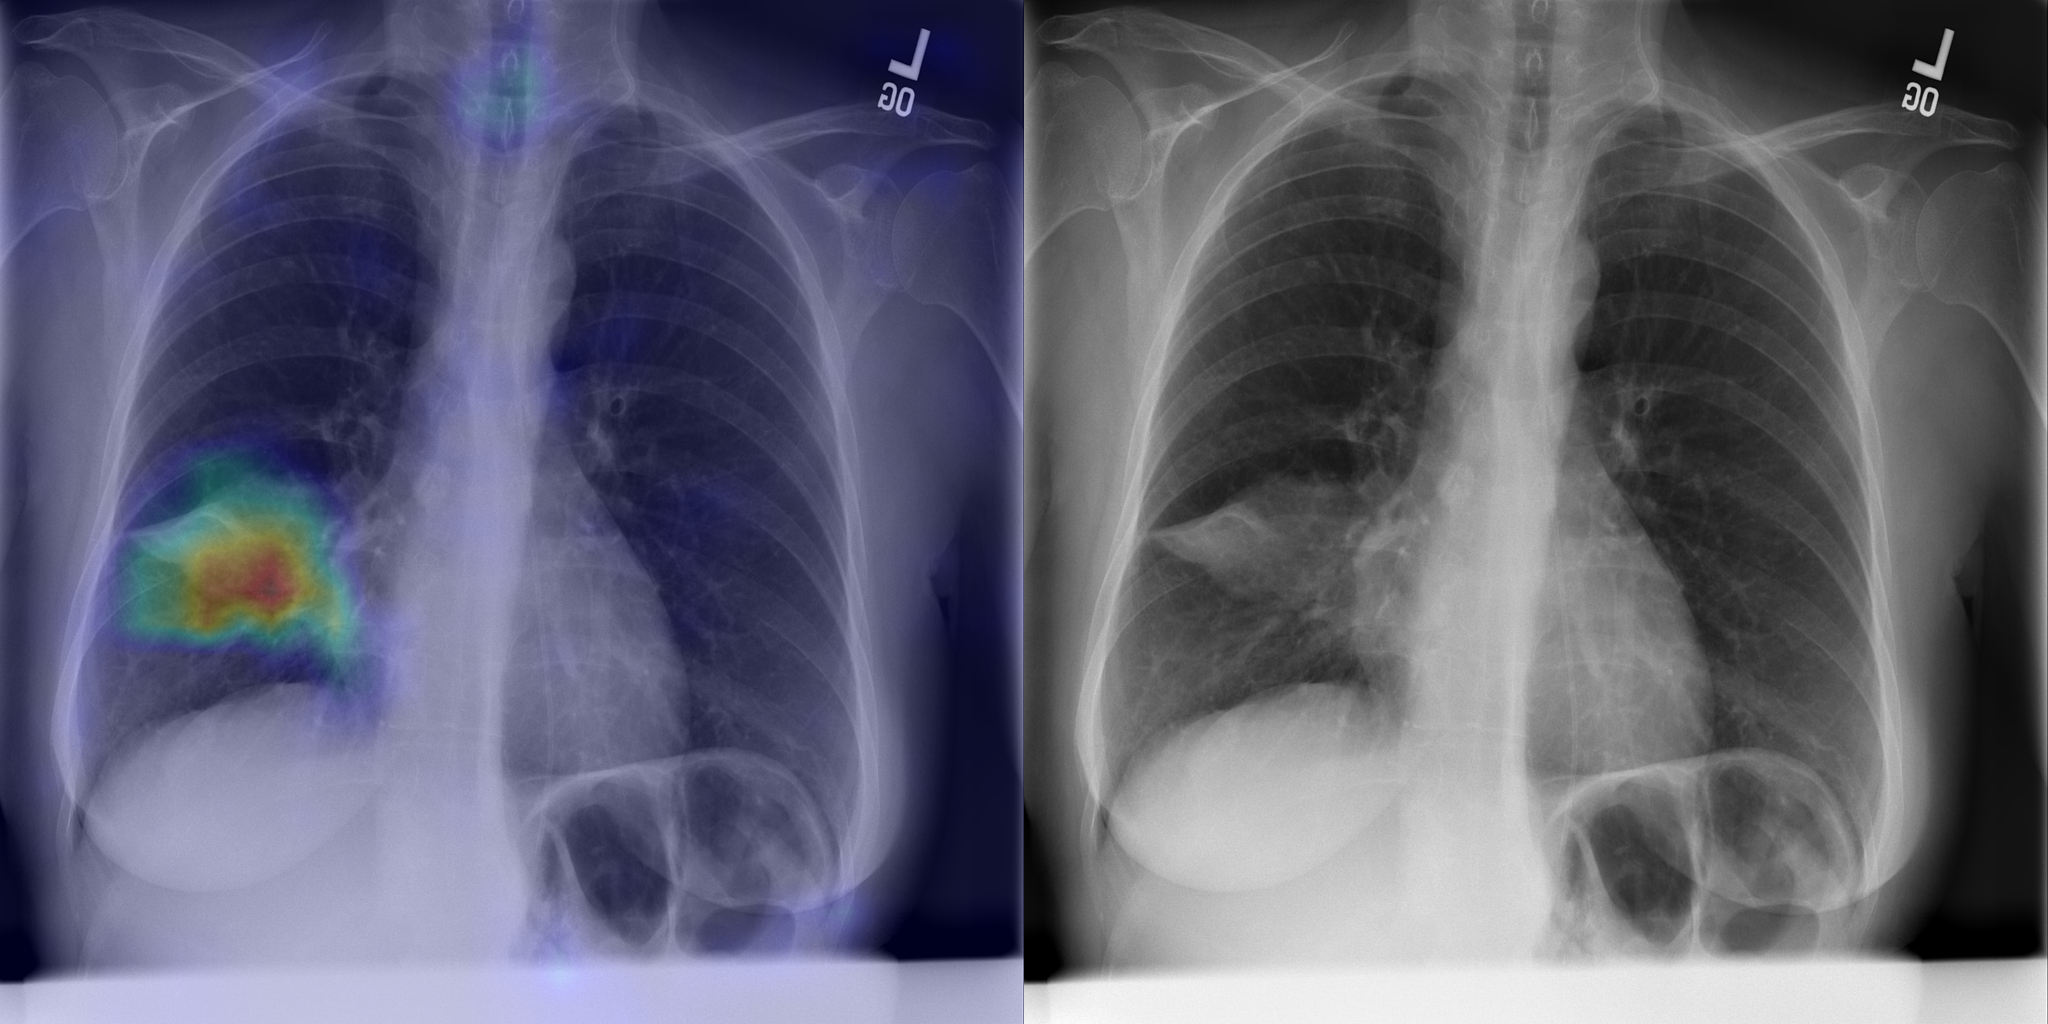
\includegraphics[width=1.0\textwidth]{Chapters/5. Conclusiones/img/Consolidation/1_1_00000618_011.png}
    \end{subfigure}
    \begin{subfigure}{0.4\textwidth}
        \centering
        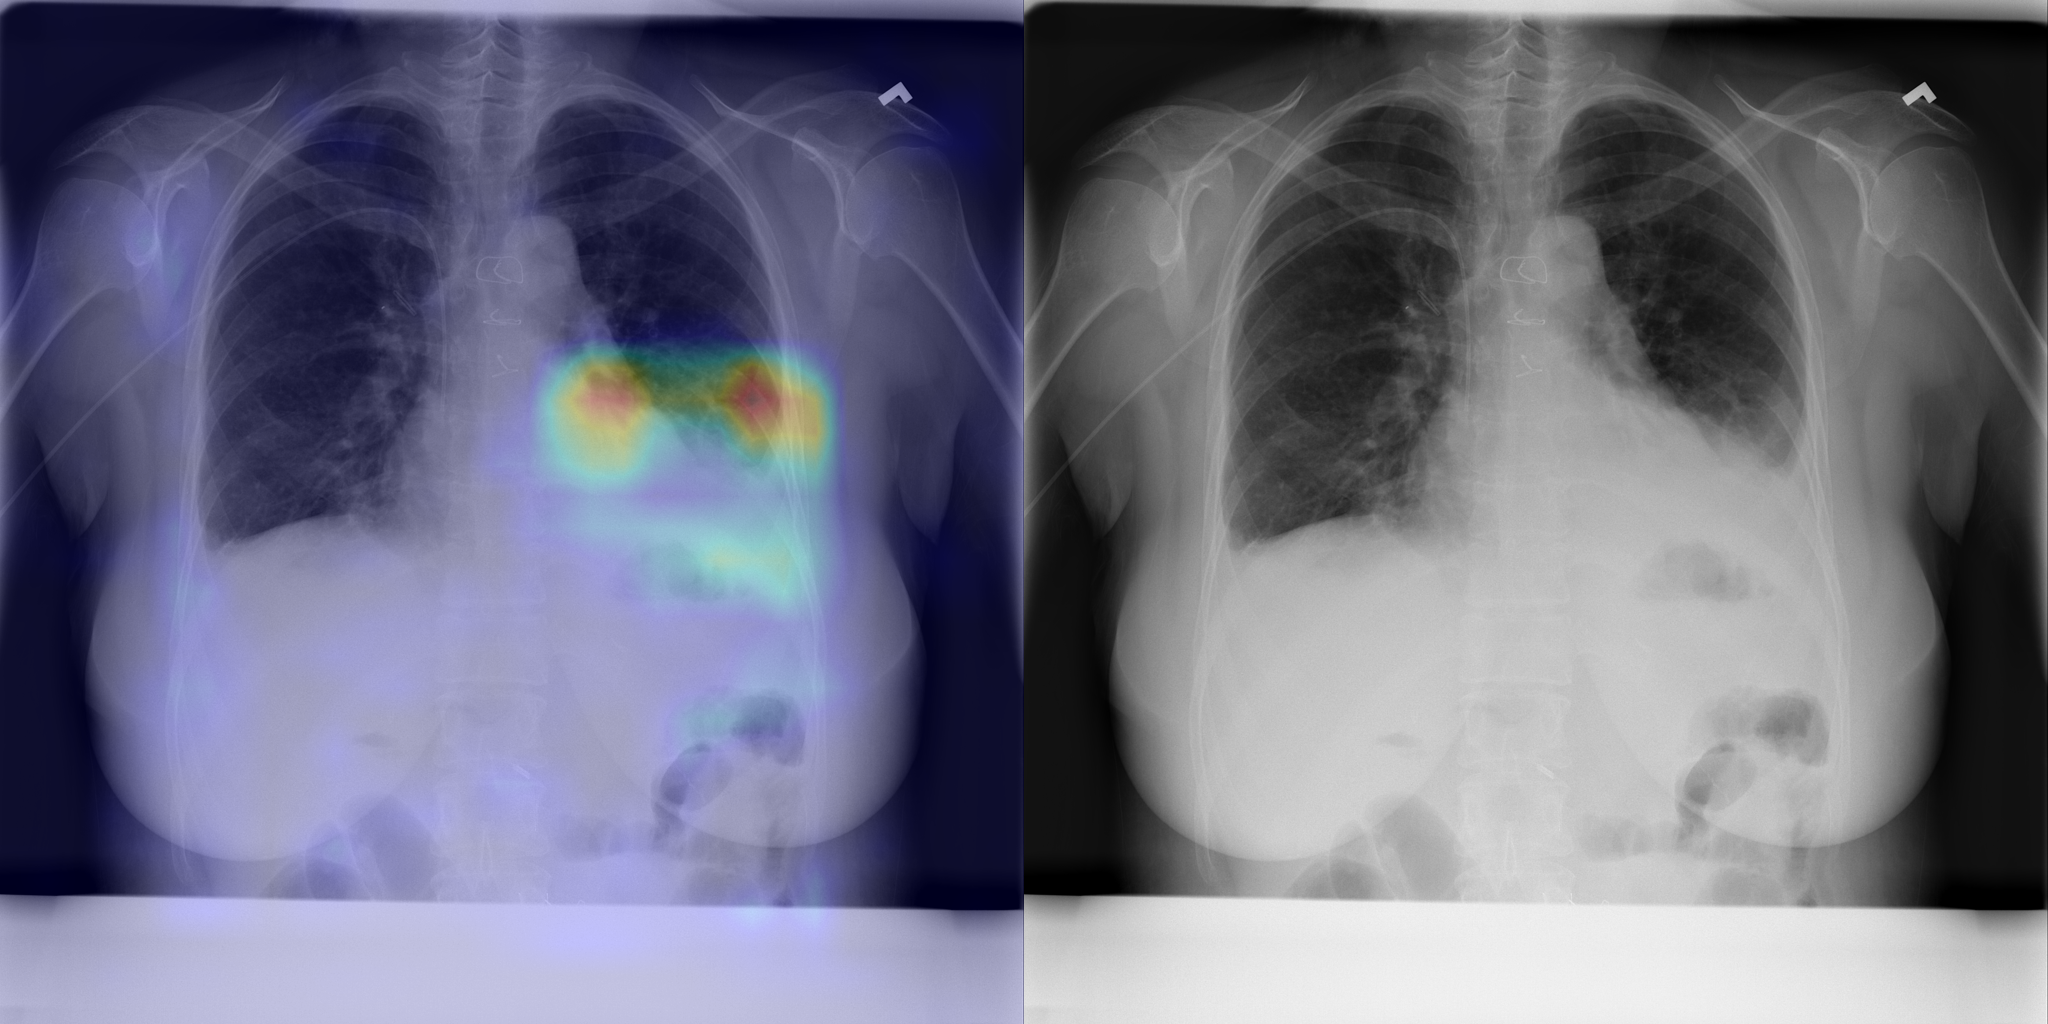
\includegraphics[width=1.0\textwidth]{Chapters/5. Conclusiones/img/Consolidation/1_1_00000808_002.png}
    \end{subfigure}
    \begin{subfigure}{0.4\textwidth}
        \centering
        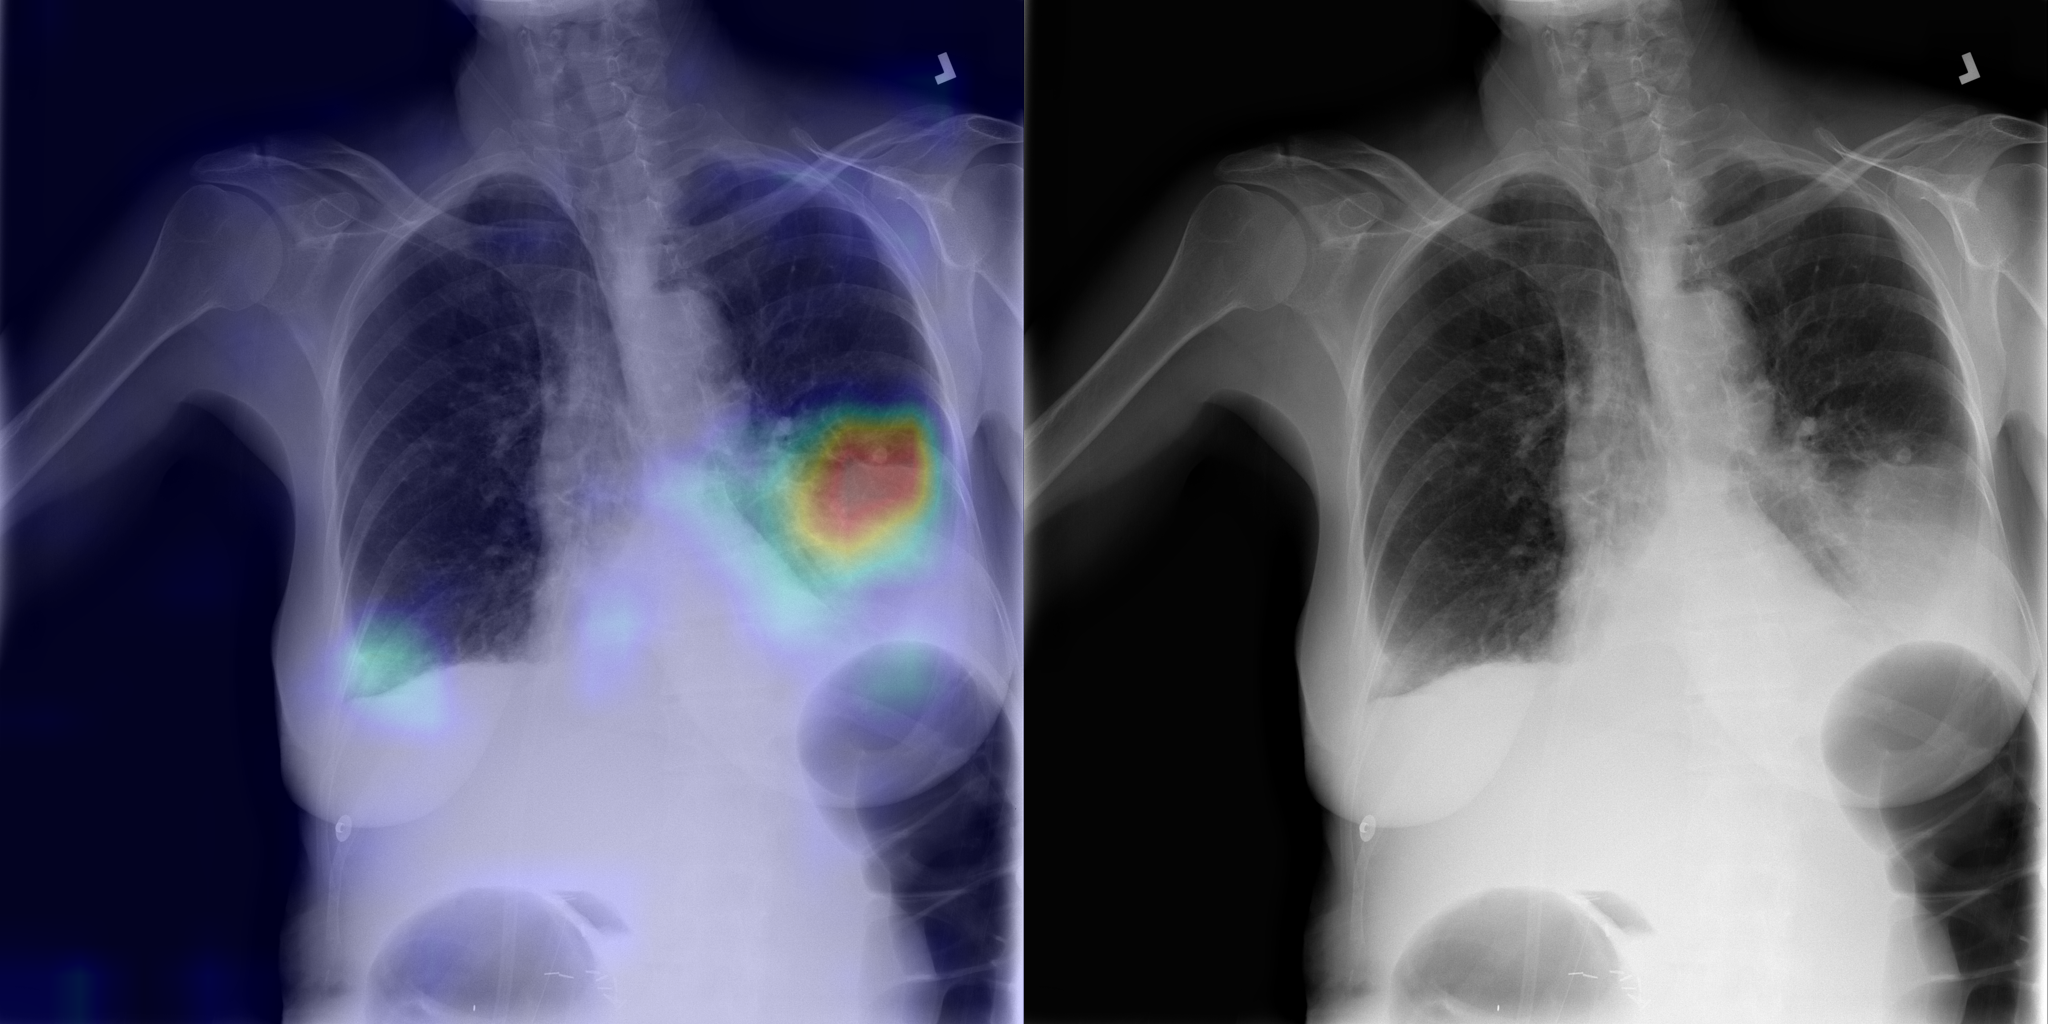
\includegraphics[width=1.0\textwidth]{Chapters/5. Conclusiones/img/Consolidation/1_1_00000882_003.png}
    \end{subfigure}
    \begin{subfigure}{0.4\textwidth}
        \centering
        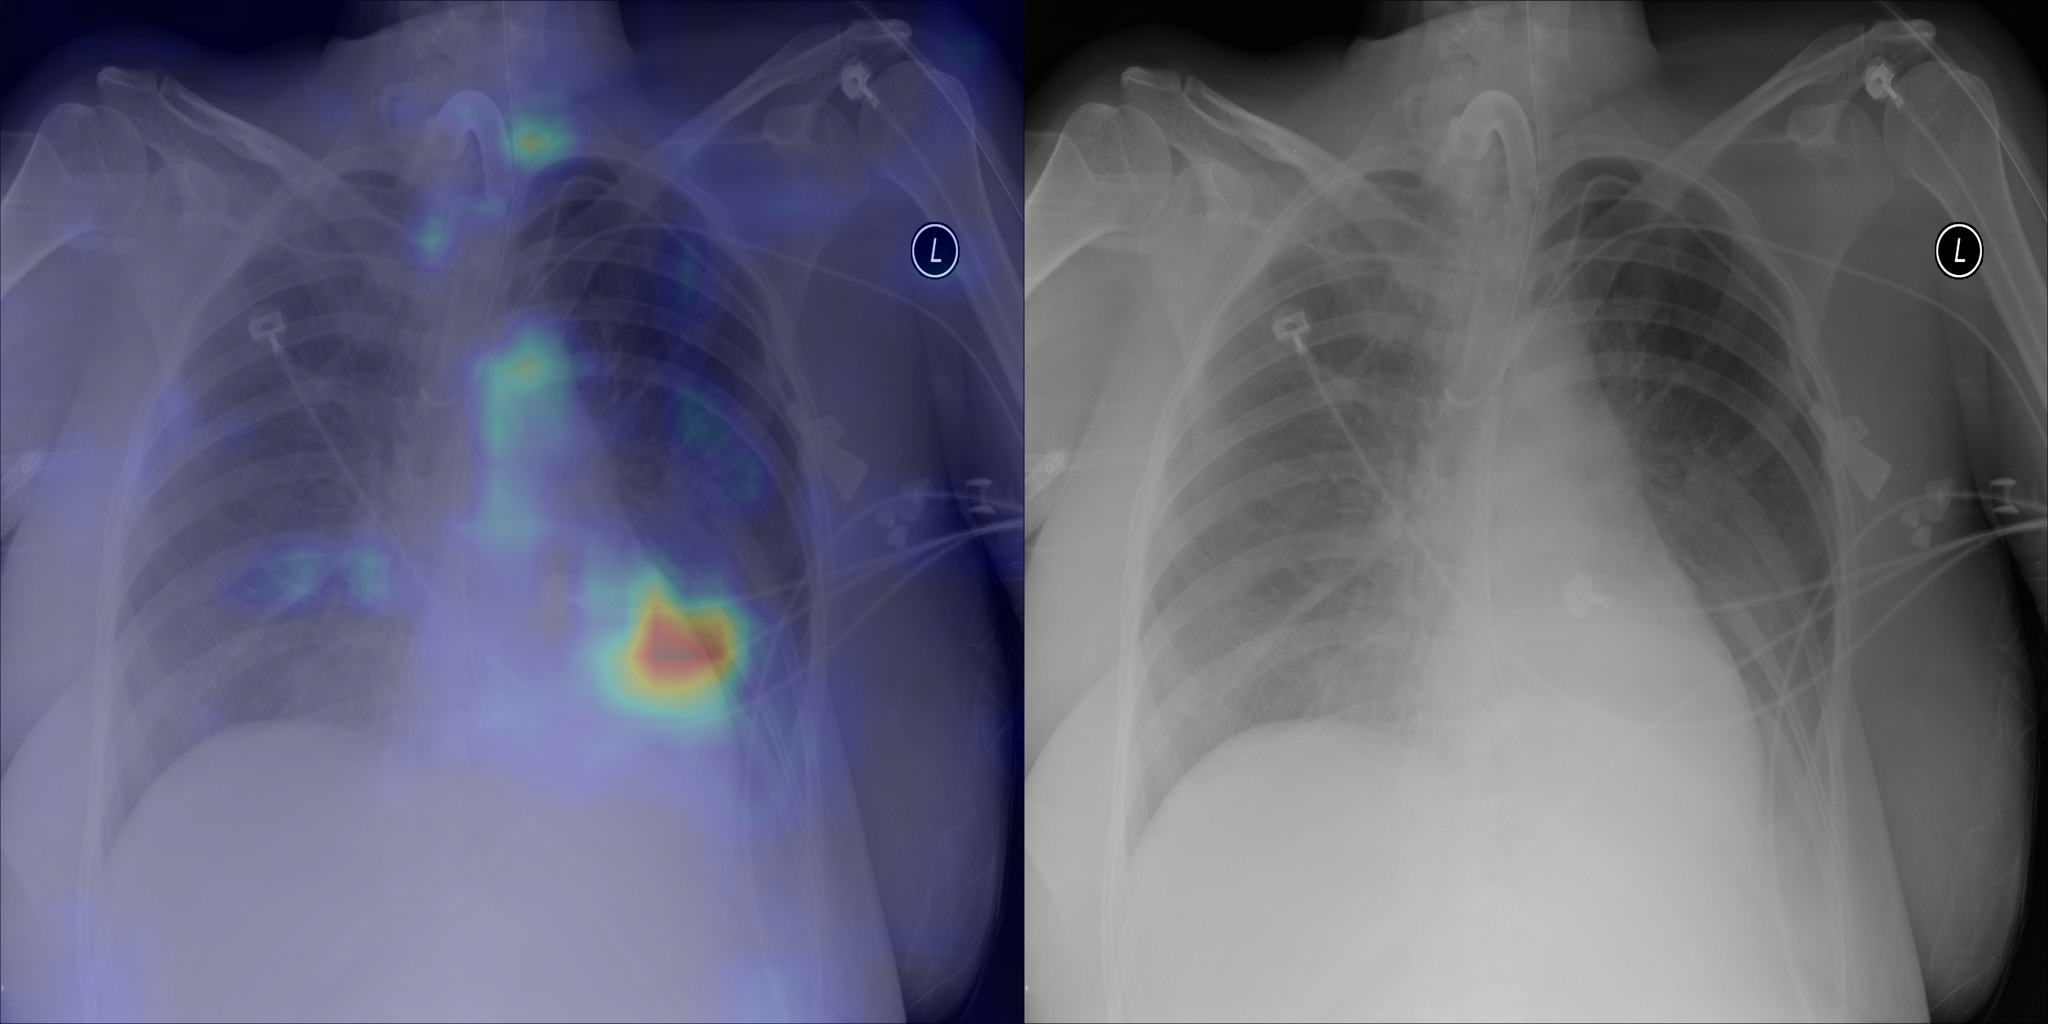
\includegraphics[width=1.0\textwidth]{Chapters/5. Conclusiones/img/Consolidation/1_1_00018187_052.png}
    \end{subfigure}

    \caption[short]{Consolidación pulmunar. Radiografías detectadas con la patología de consolidación pulmunar por los
                    radiólogos. A la izquierda de cada imagen el GradCam correspondiente a la detección
                    de la patología como positivo por el modelo CNN.}
\end{figure}

\begin{figure}[b]
    \centering
    \begin{subfigure}{0.4\textwidth}
        \centering
        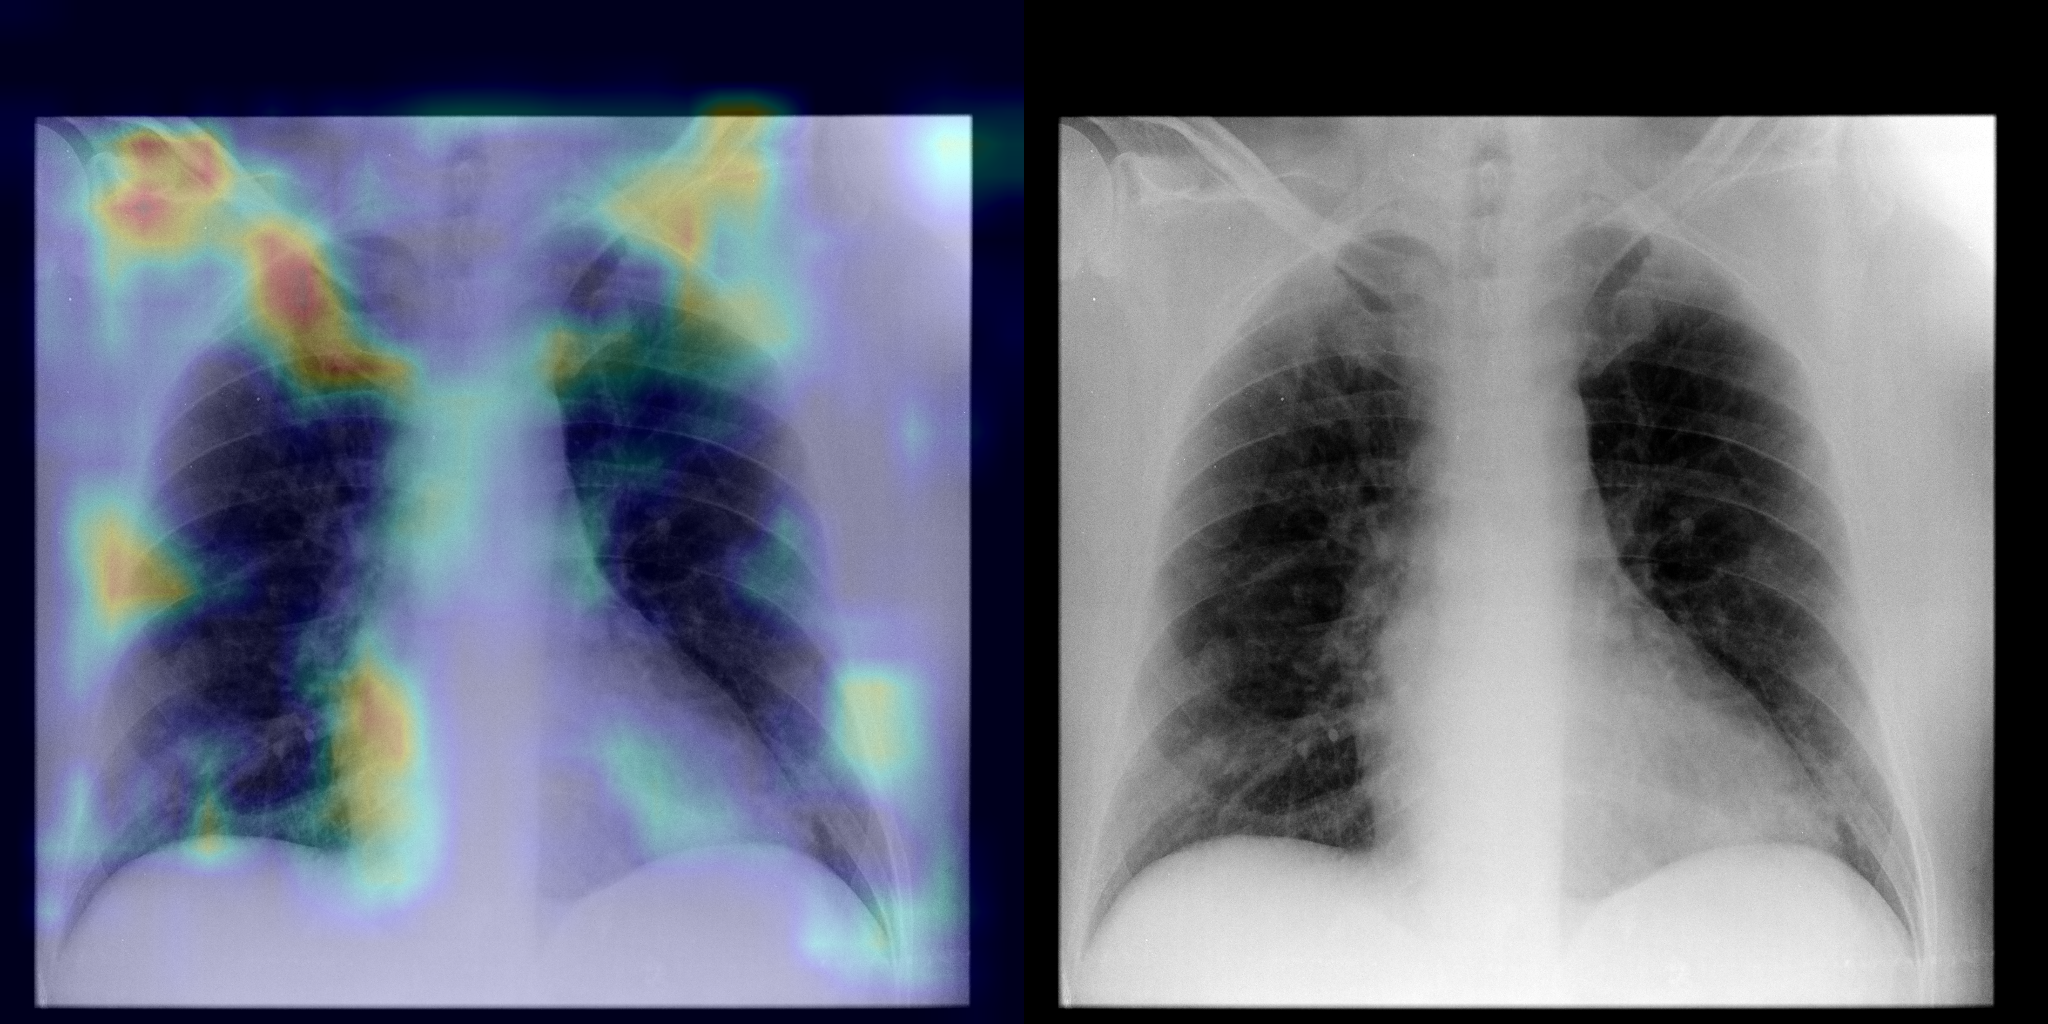
\includegraphics[width=1.0\textwidth]{Chapters/5. Conclusiones/img/COVID-19/1_1_0c9b15035c41_3ea703bd1e0b.png}
    \end{subfigure}
    \begin{subfigure}{0.4\textwidth}
        \centering
        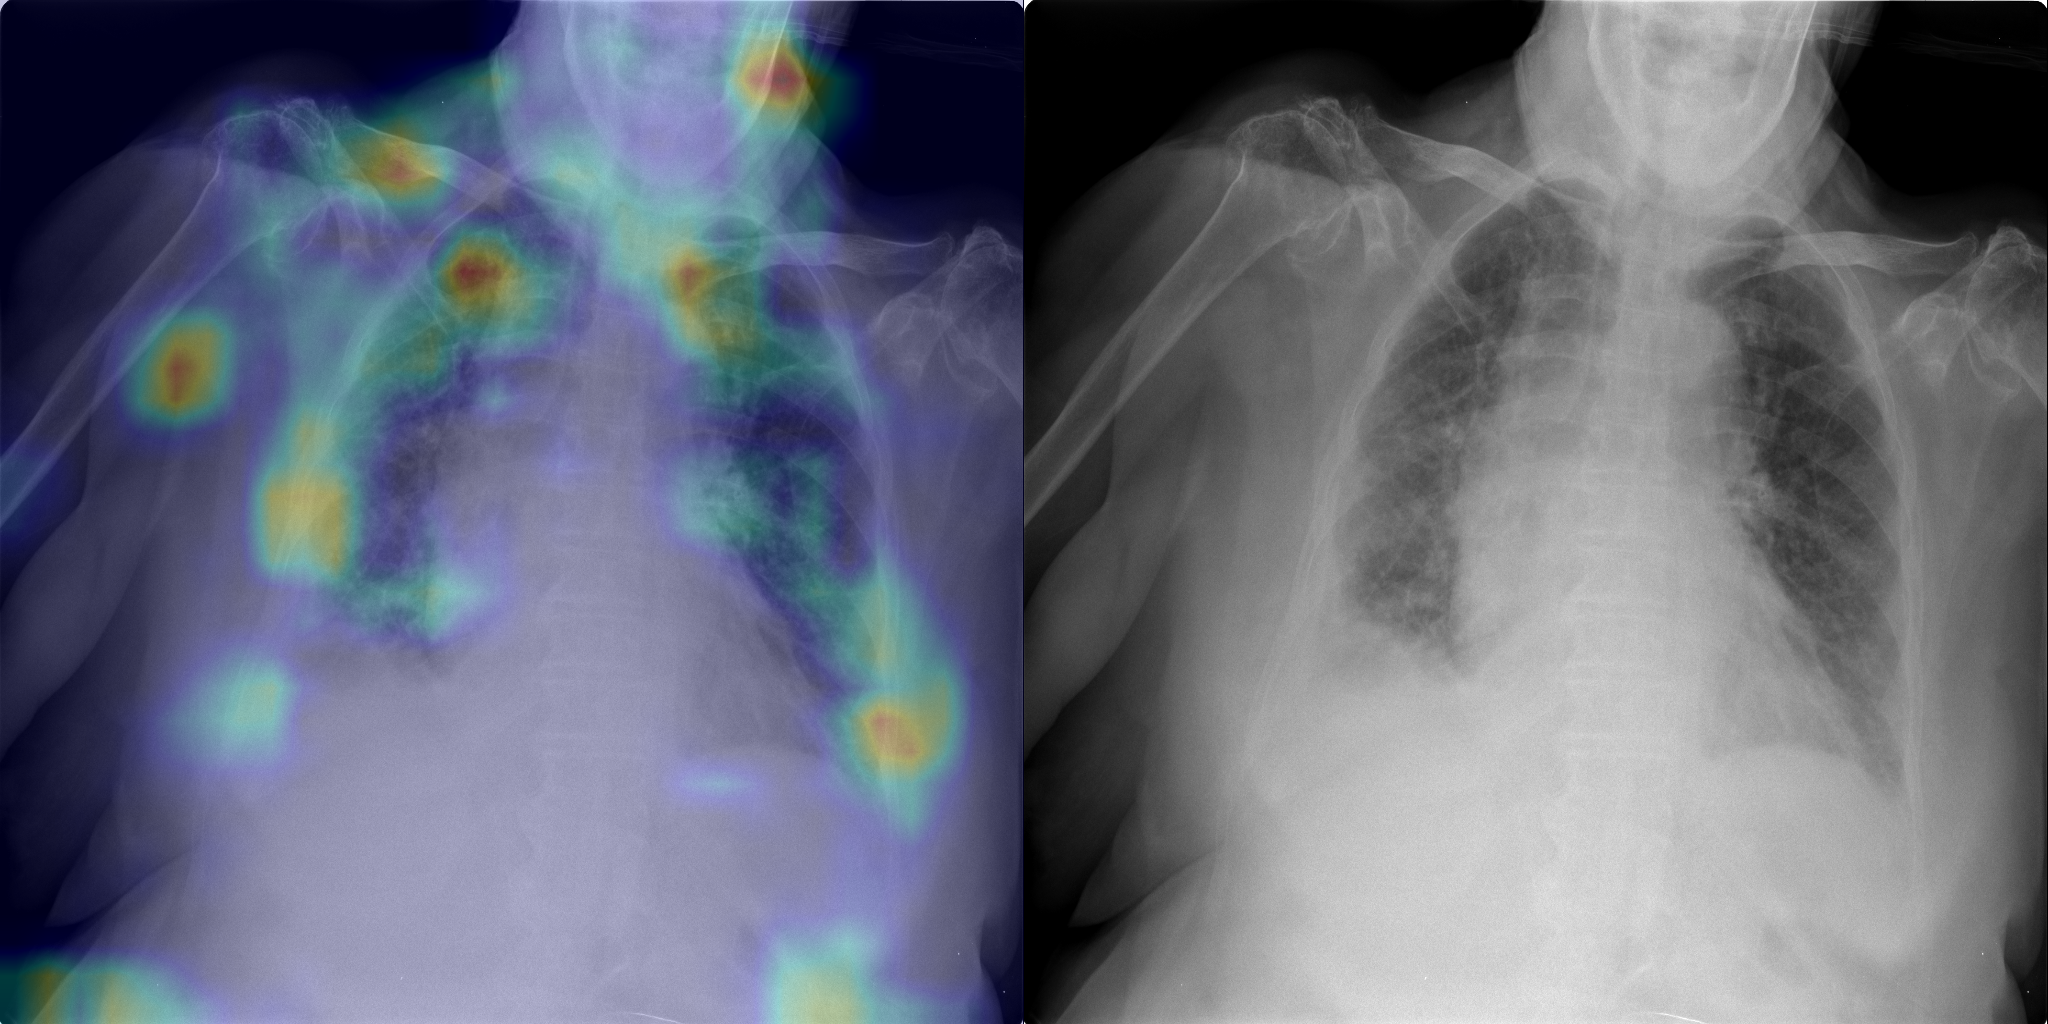
\includegraphics[width=1.0\textwidth]{Chapters/5. Conclusiones/img/COVID-19/1_1_0d5082a9a044_d417f8e64511.png}
    \end{subfigure}
    \begin{subfigure}{0.4\textwidth}
        \centering
        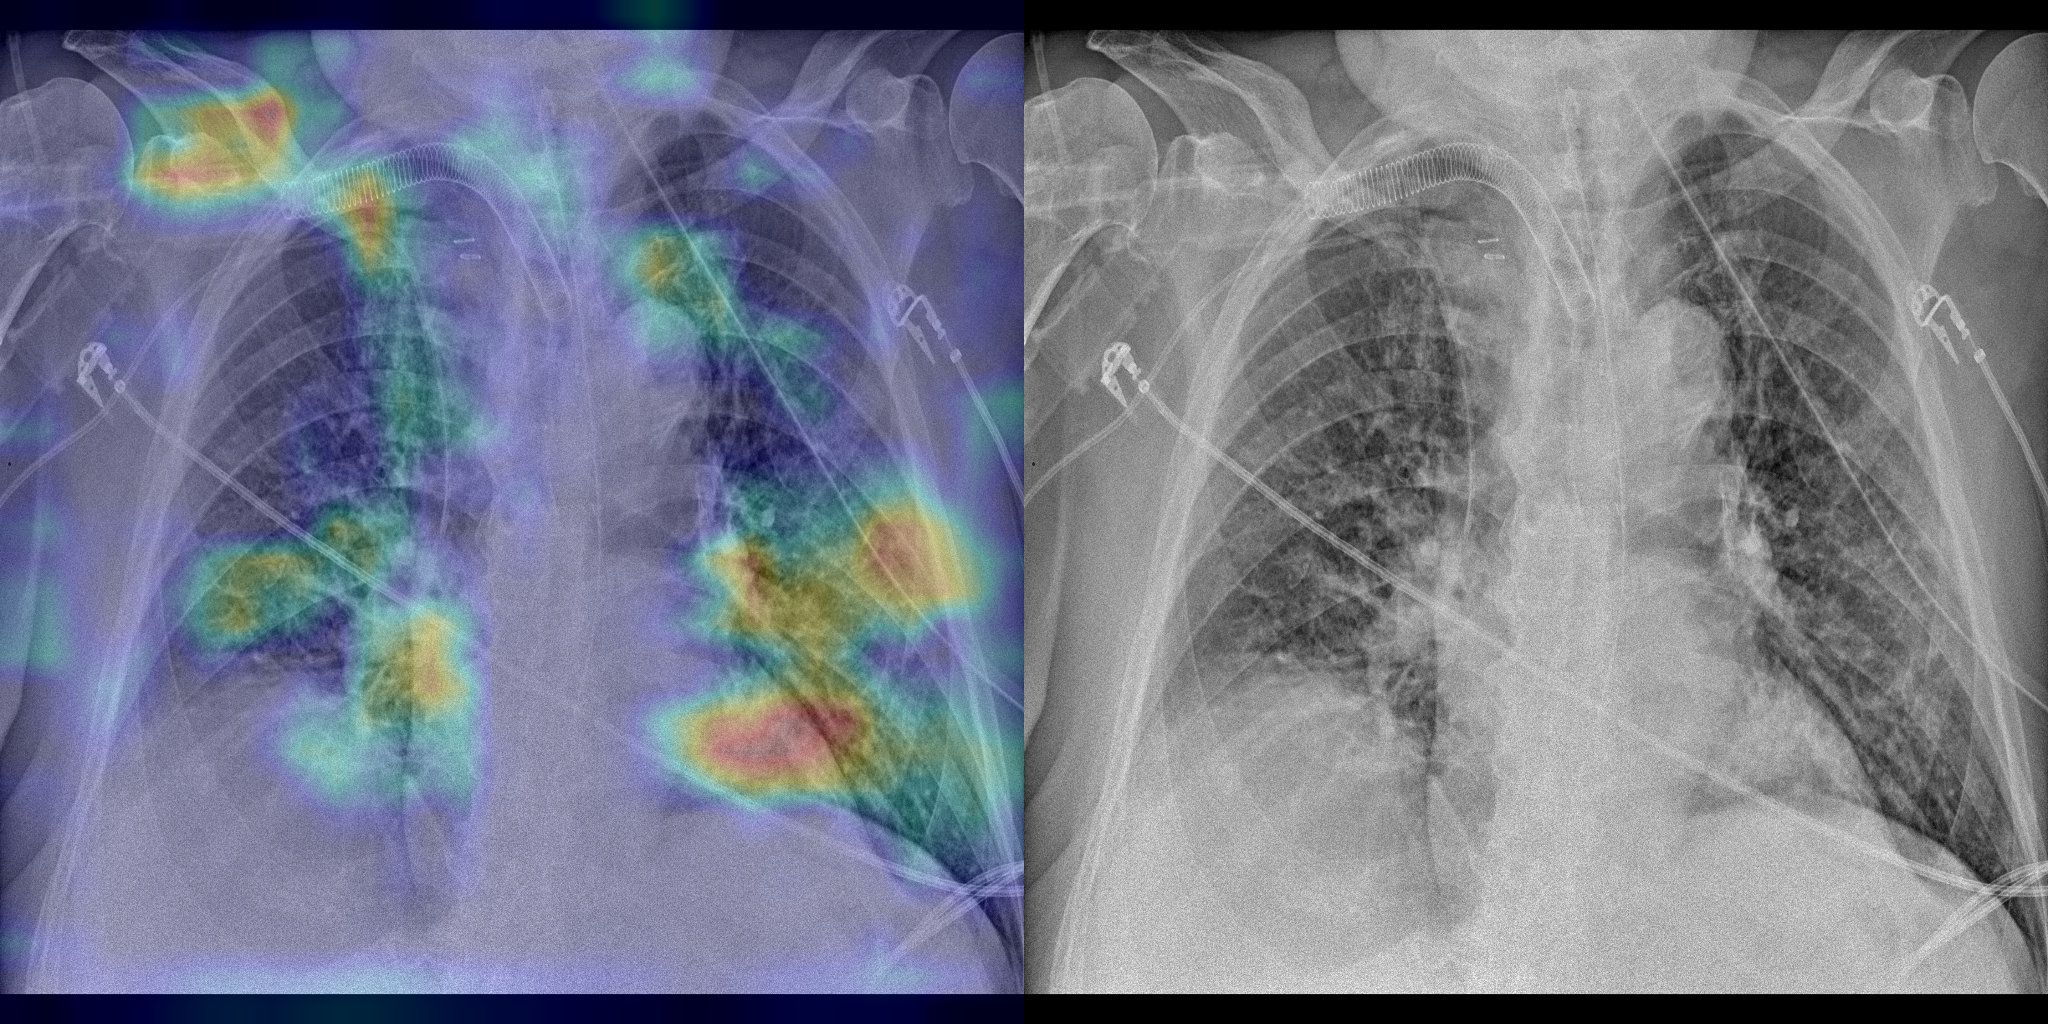
\includegraphics[width=1.0\textwidth]{Chapters/5. Conclusiones/img/COVID-19/1_1_1b5ca94ac38b_68fcf433c6fe.png}
    \end{subfigure}
    \begin{subfigure}{0.4\textwidth}
        \centering
        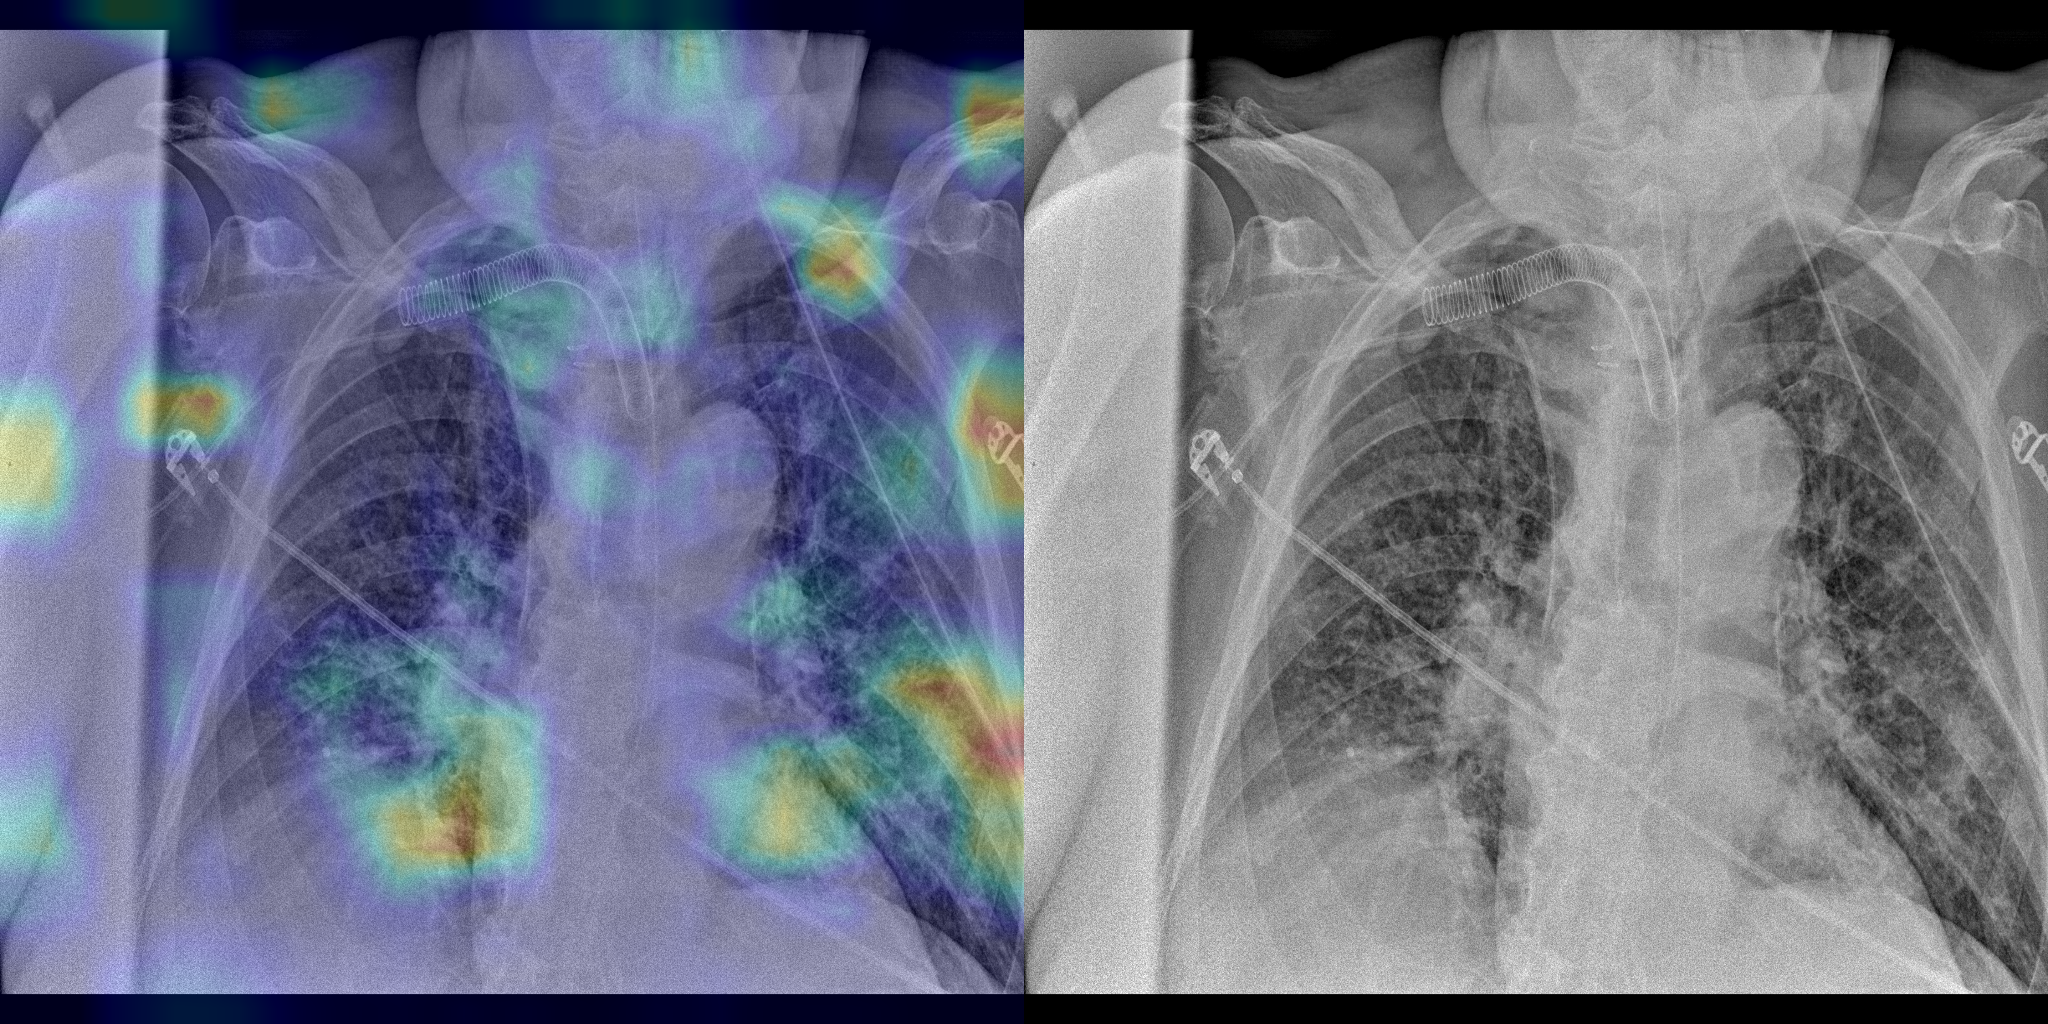
\includegraphics[width=1.0\textwidth]{Chapters/5. Conclusiones/img/COVID-19/1_1_1b5ca94ac38b_0919a3b8af01.png}
    \end{subfigure}
    \begin{subfigure}{0.4\textwidth}
        \centering
        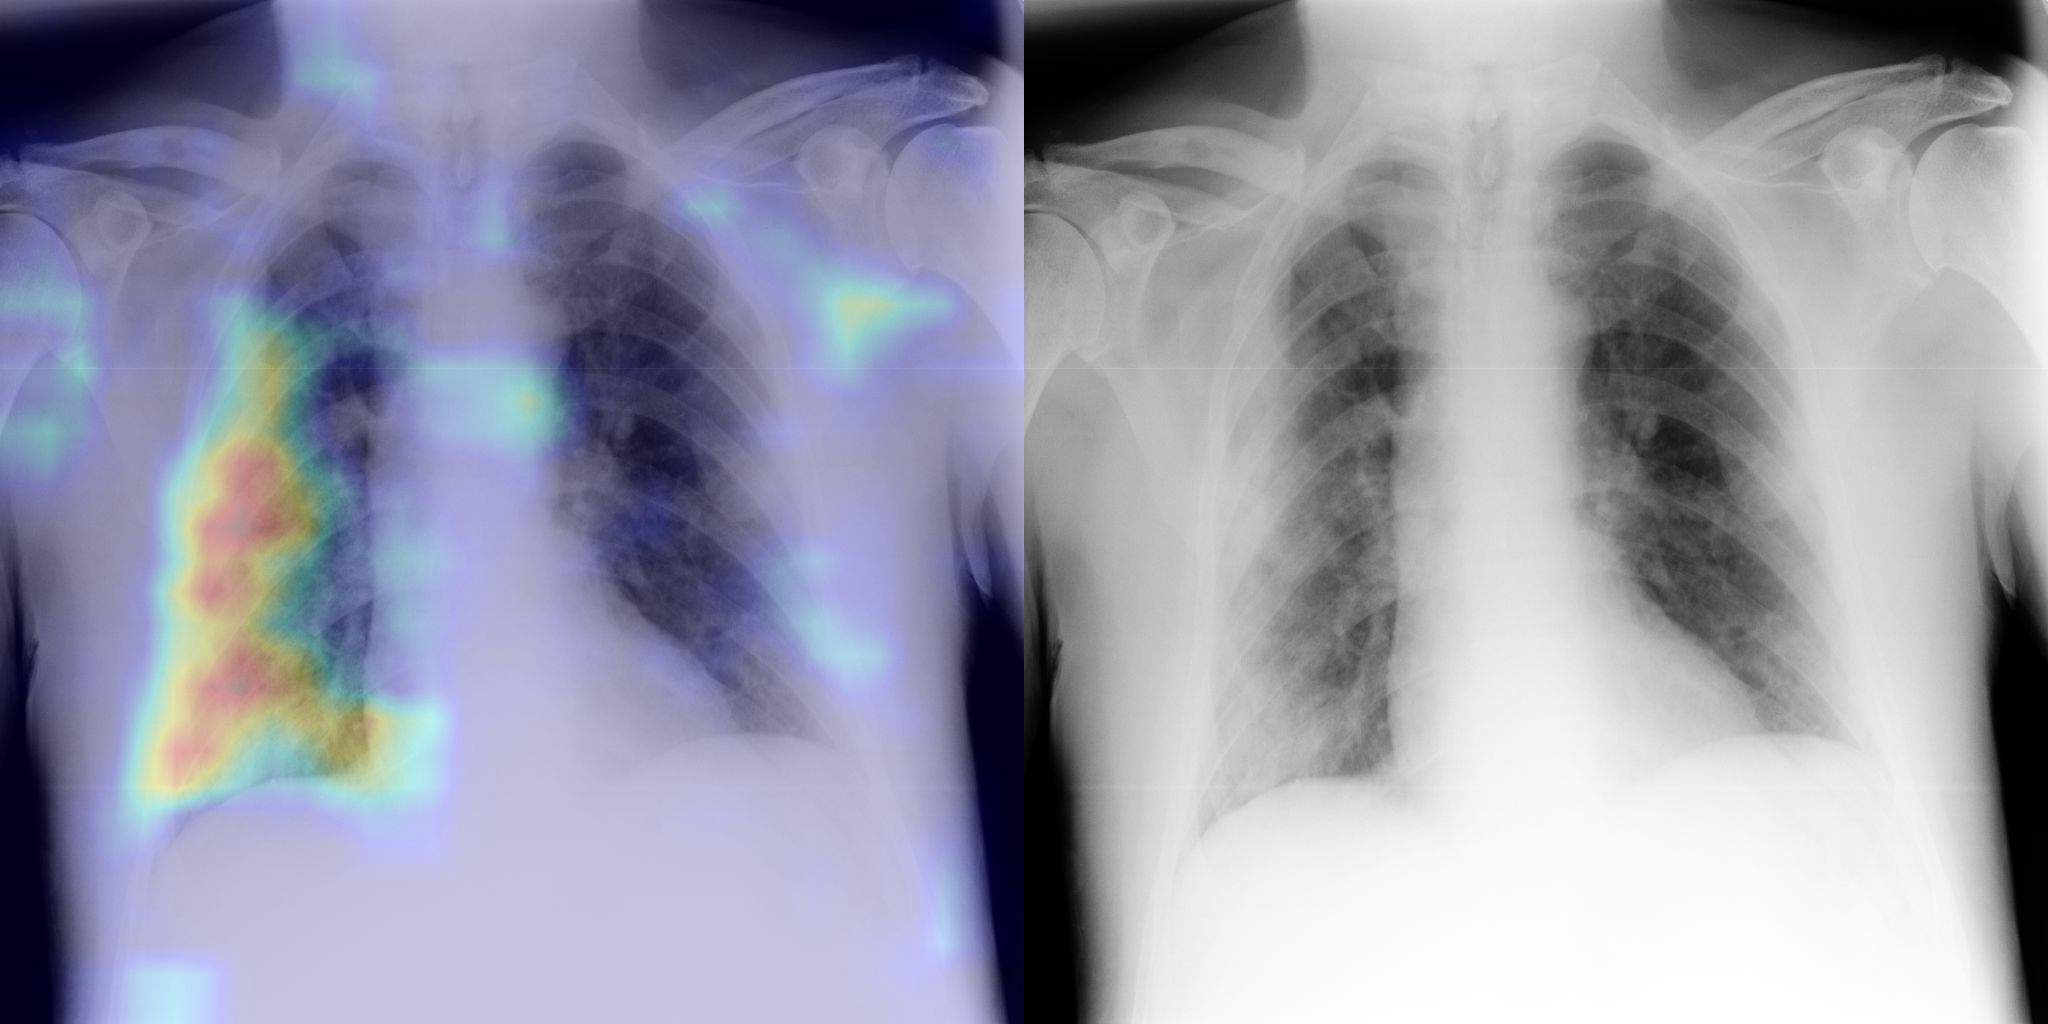
\includegraphics[width=1.0\textwidth]{Chapters/5. Conclusiones/img/COVID-19/1_1_1e3f6f8e494c_efe83e860c17.png}
    \end{subfigure}
    \begin{subfigure}{0.4\textwidth}
        \centering
        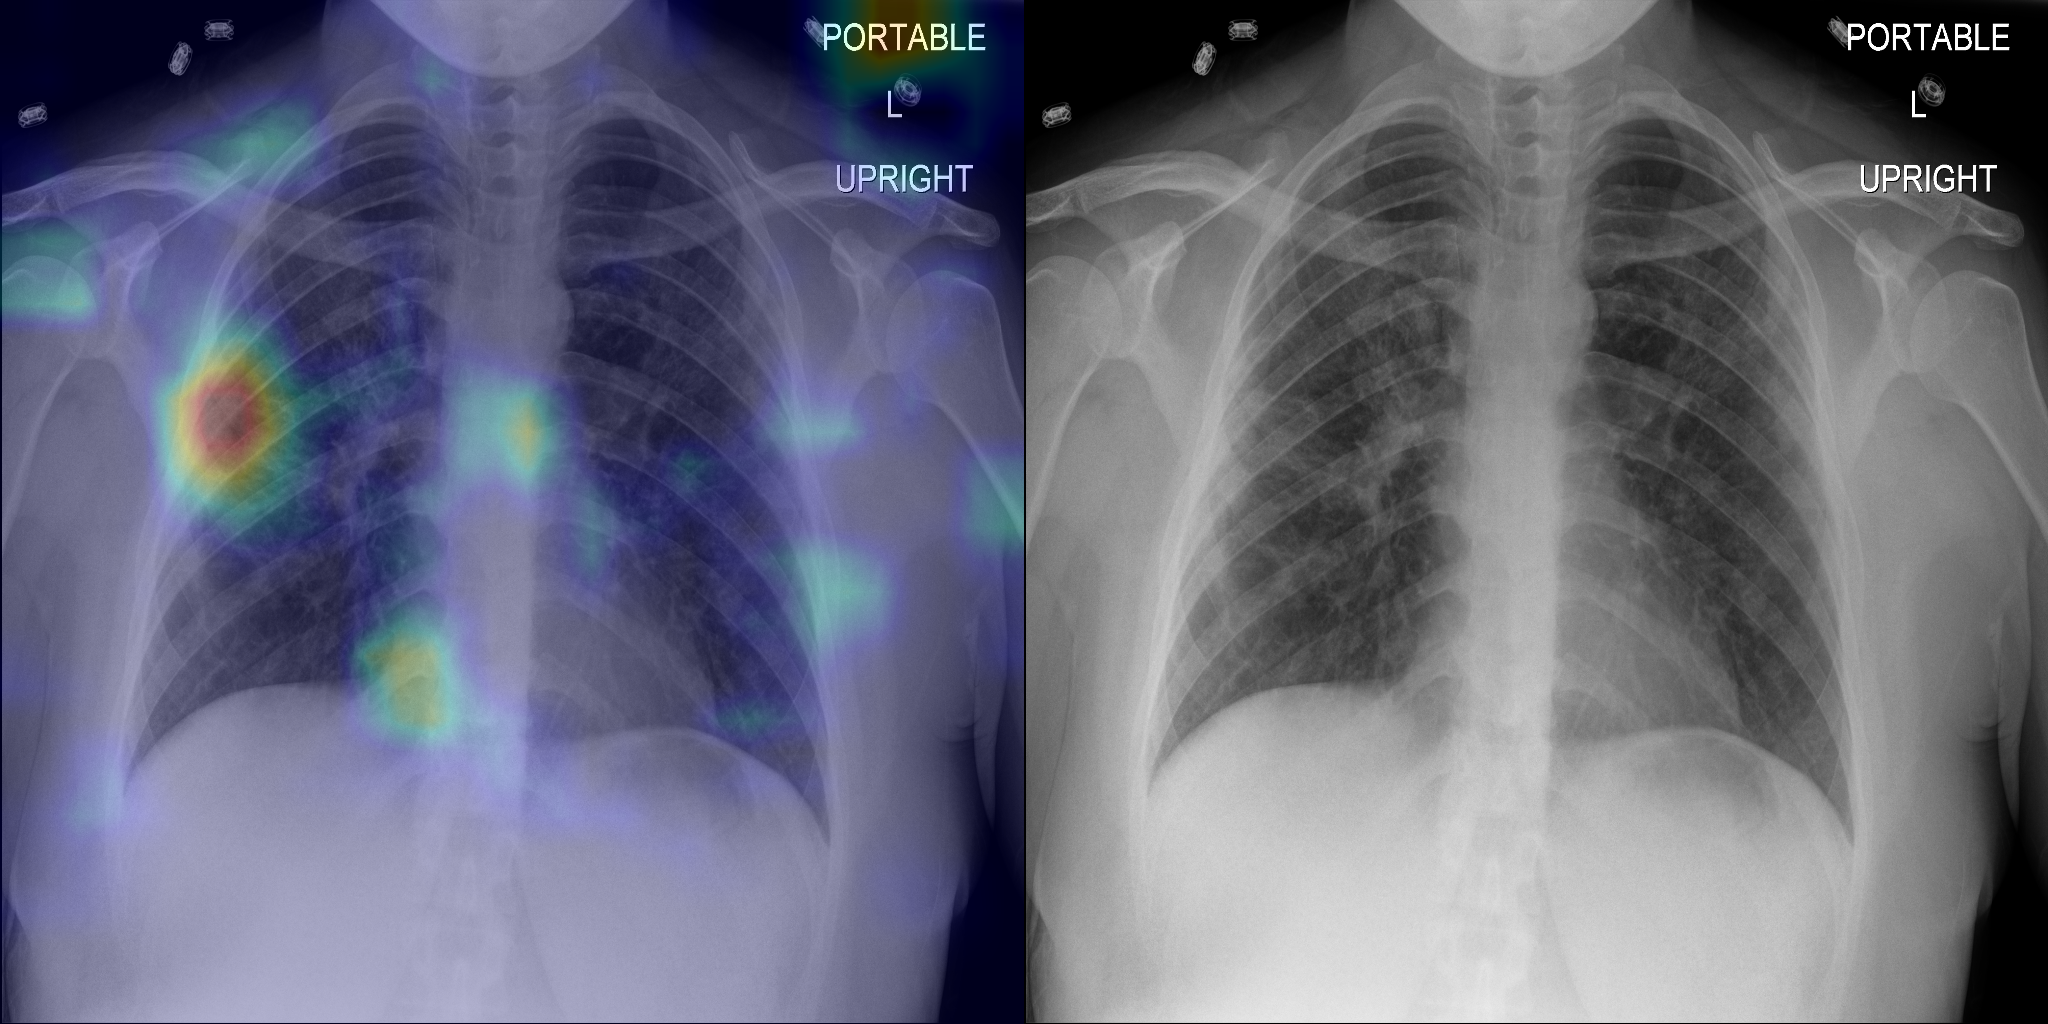
\includegraphics[width=1.0\textwidth]{Chapters/5. Conclusiones/img/COVID-19/1_1_4bb14a344446_0d3910133fbe.png}
    \end{subfigure}
    \begin{subfigure}{0.4\textwidth}
        \centering
        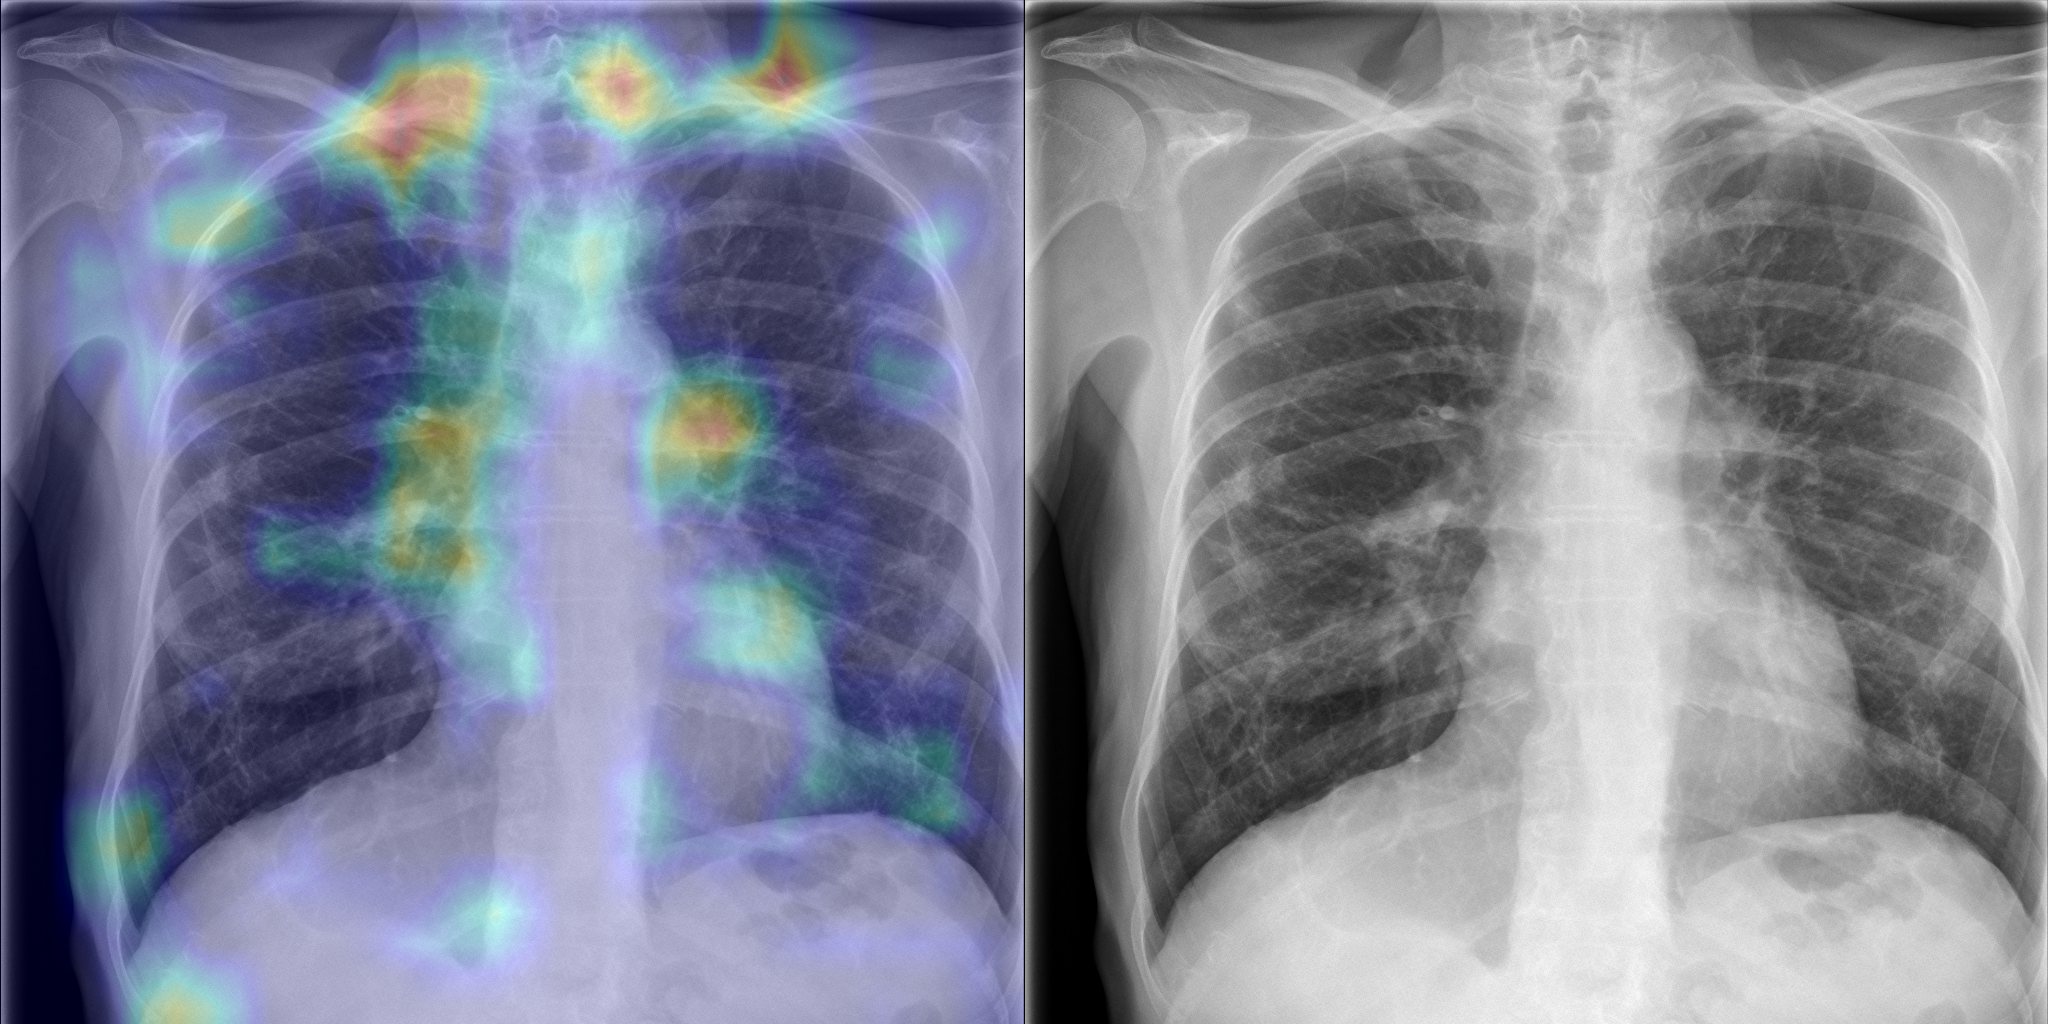
\includegraphics[width=1.0\textwidth]{Chapters/5. Conclusiones/img/COVID-19/1_1_4be426760e00_16d85c7f7837.png}
    \end{subfigure}
    \begin{subfigure}{0.4\textwidth}
        \centering
        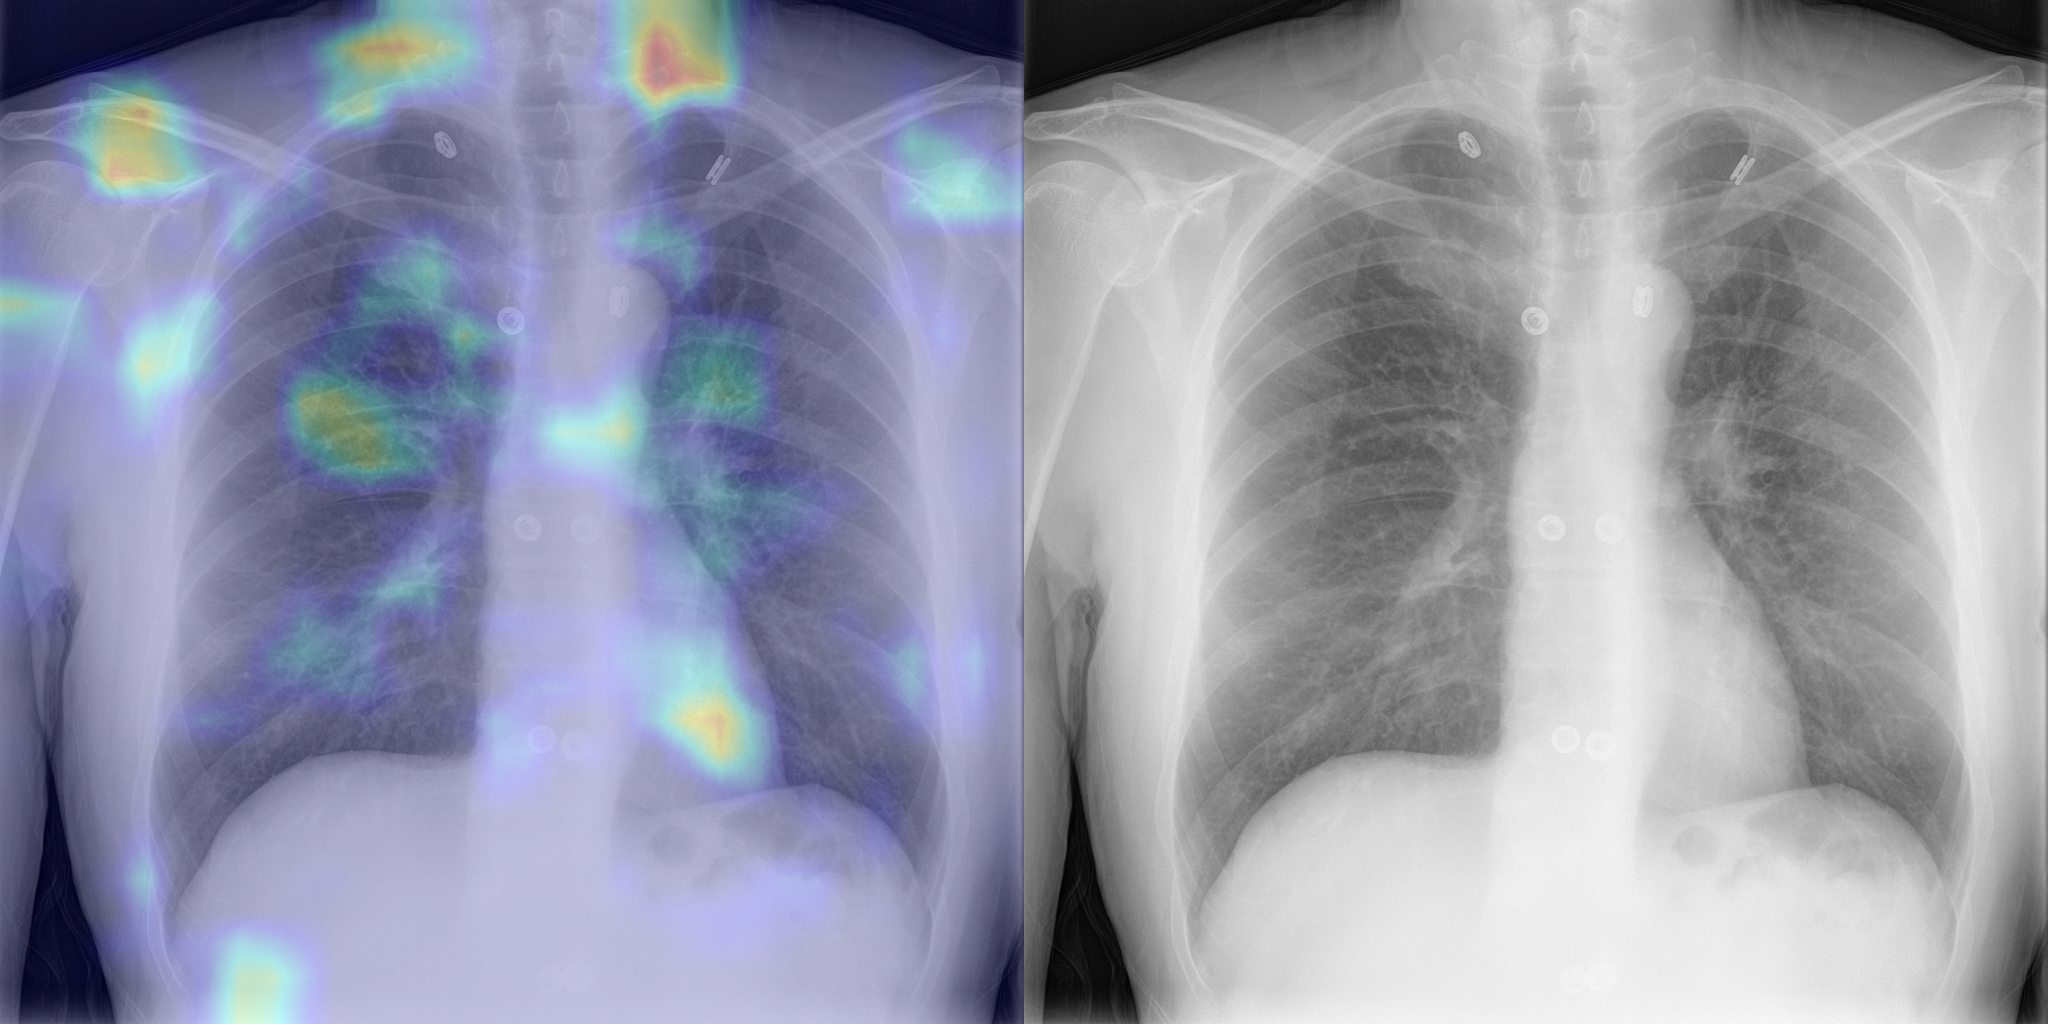
\includegraphics[width=1.0\textwidth]{Chapters/5. Conclusiones/img/COVID-19/1_1_7b6c49da06db_b6b631939d4f.png}
    \end{subfigure}
    \begin{subfigure}{0.4\textwidth}
        \centering
        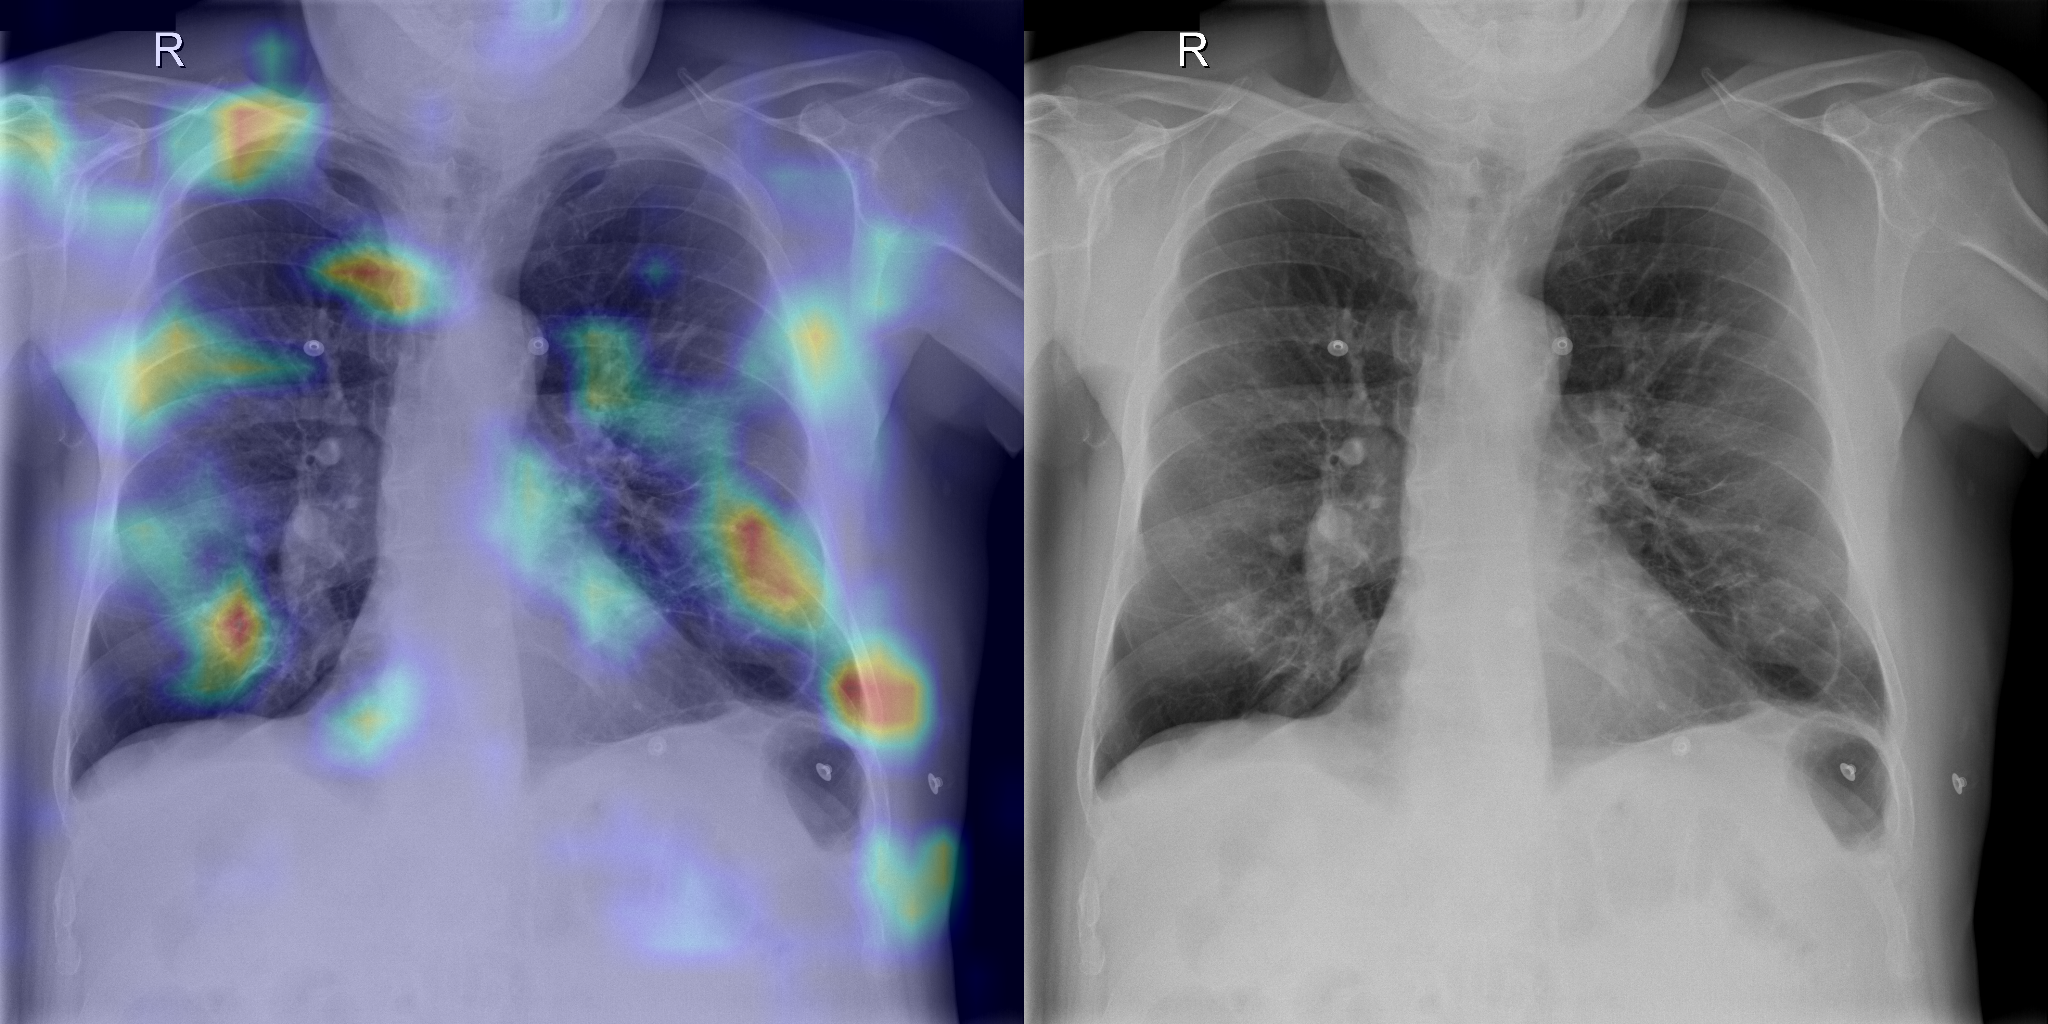
\includegraphics[width=1.0\textwidth]{Chapters/5. Conclusiones/img/COVID-19/1_1_cde0ab9526da_fa935d855d4e.png}
    \end{subfigure}
    \begin{subfigure}{0.4\textwidth}
        \centering
        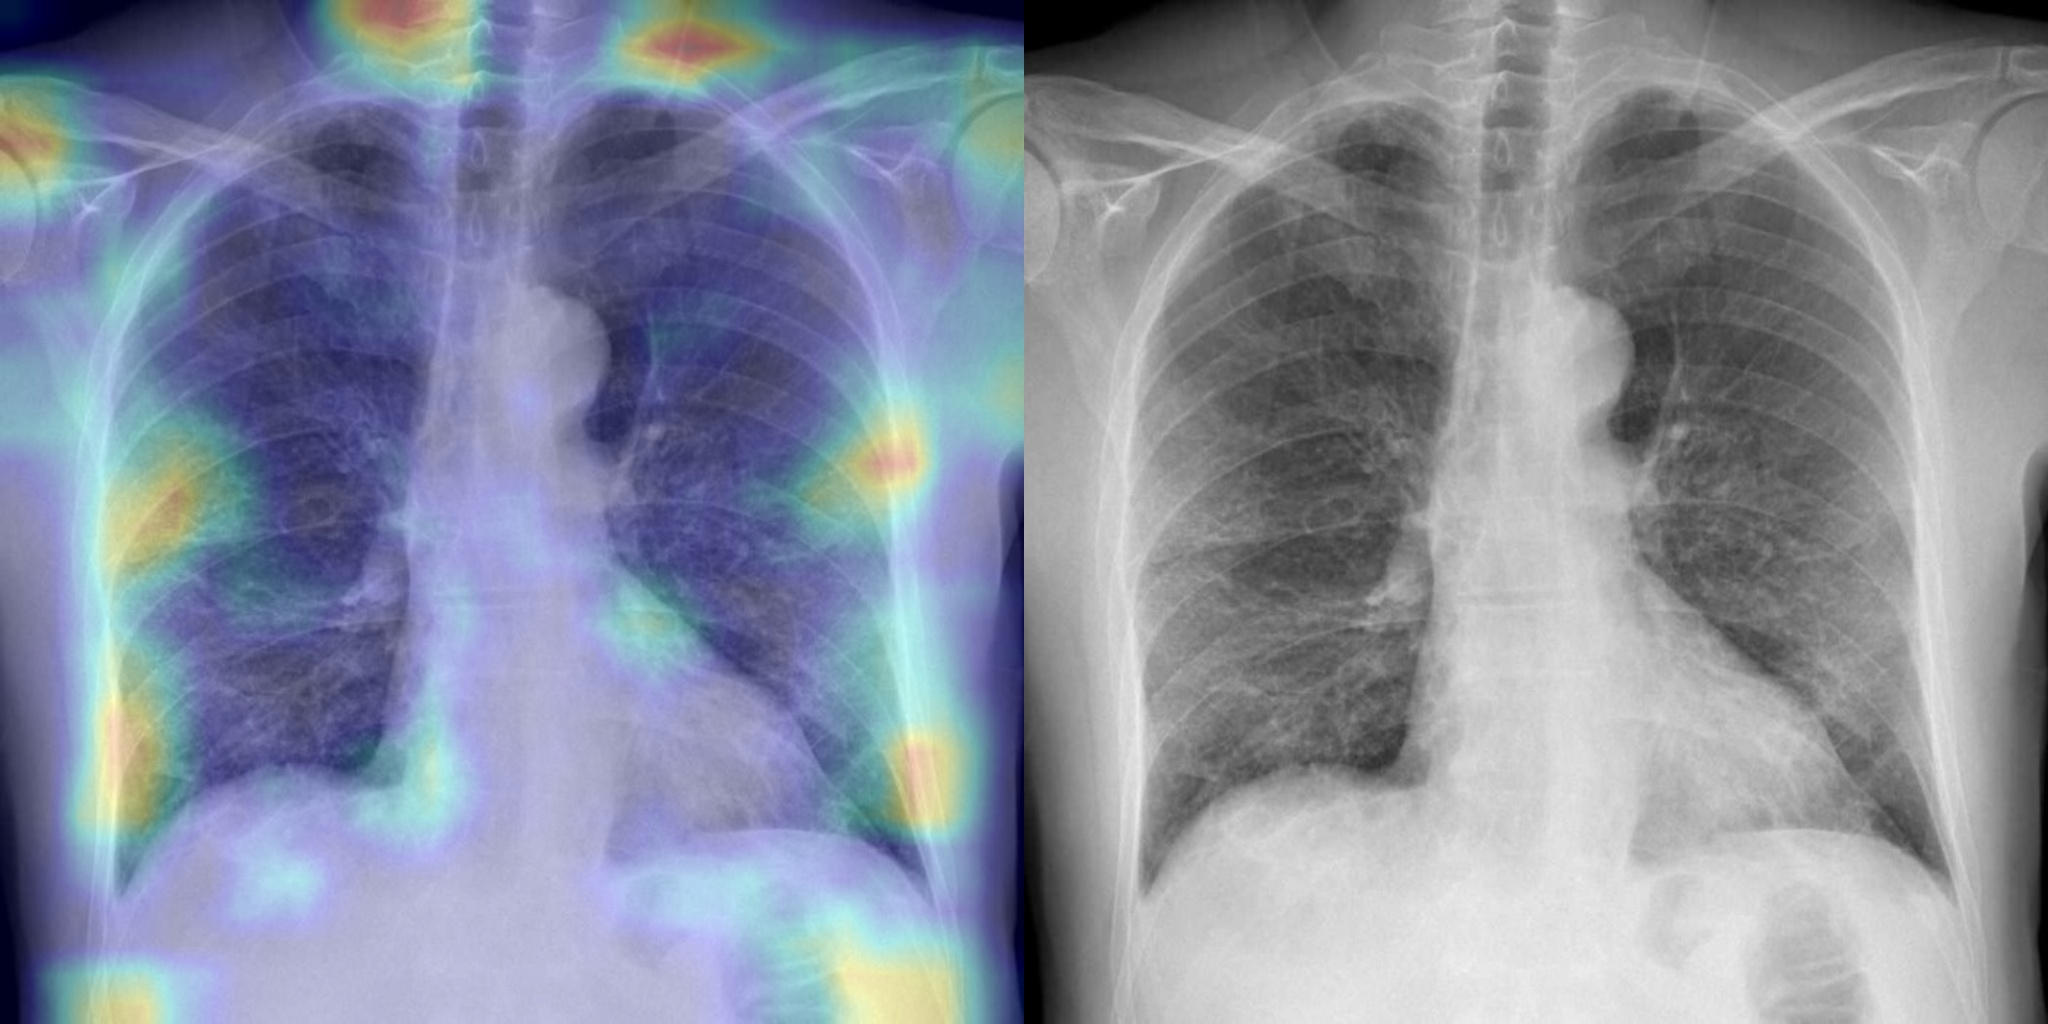
\includegraphics[width=1.0\textwidth]{Chapters/5. Conclusiones/img/COVID-19/1_1_covid-19-pneumonia-20-pa-on-admission.jpg}
    \end{subfigure}

    \caption[short]{Covid-19. Radiografías detectadas con la patología de Covid-19 por los
                    radiólogos. A la izquierda de cada imagen el GradCam correspondiente a la detección
                    de la patología como positivo por el modelo CNN.}
\end{figure}

\begin{figure}[b]
    \centering
    \begin{subfigure}{0.4\textwidth}
        \centering
        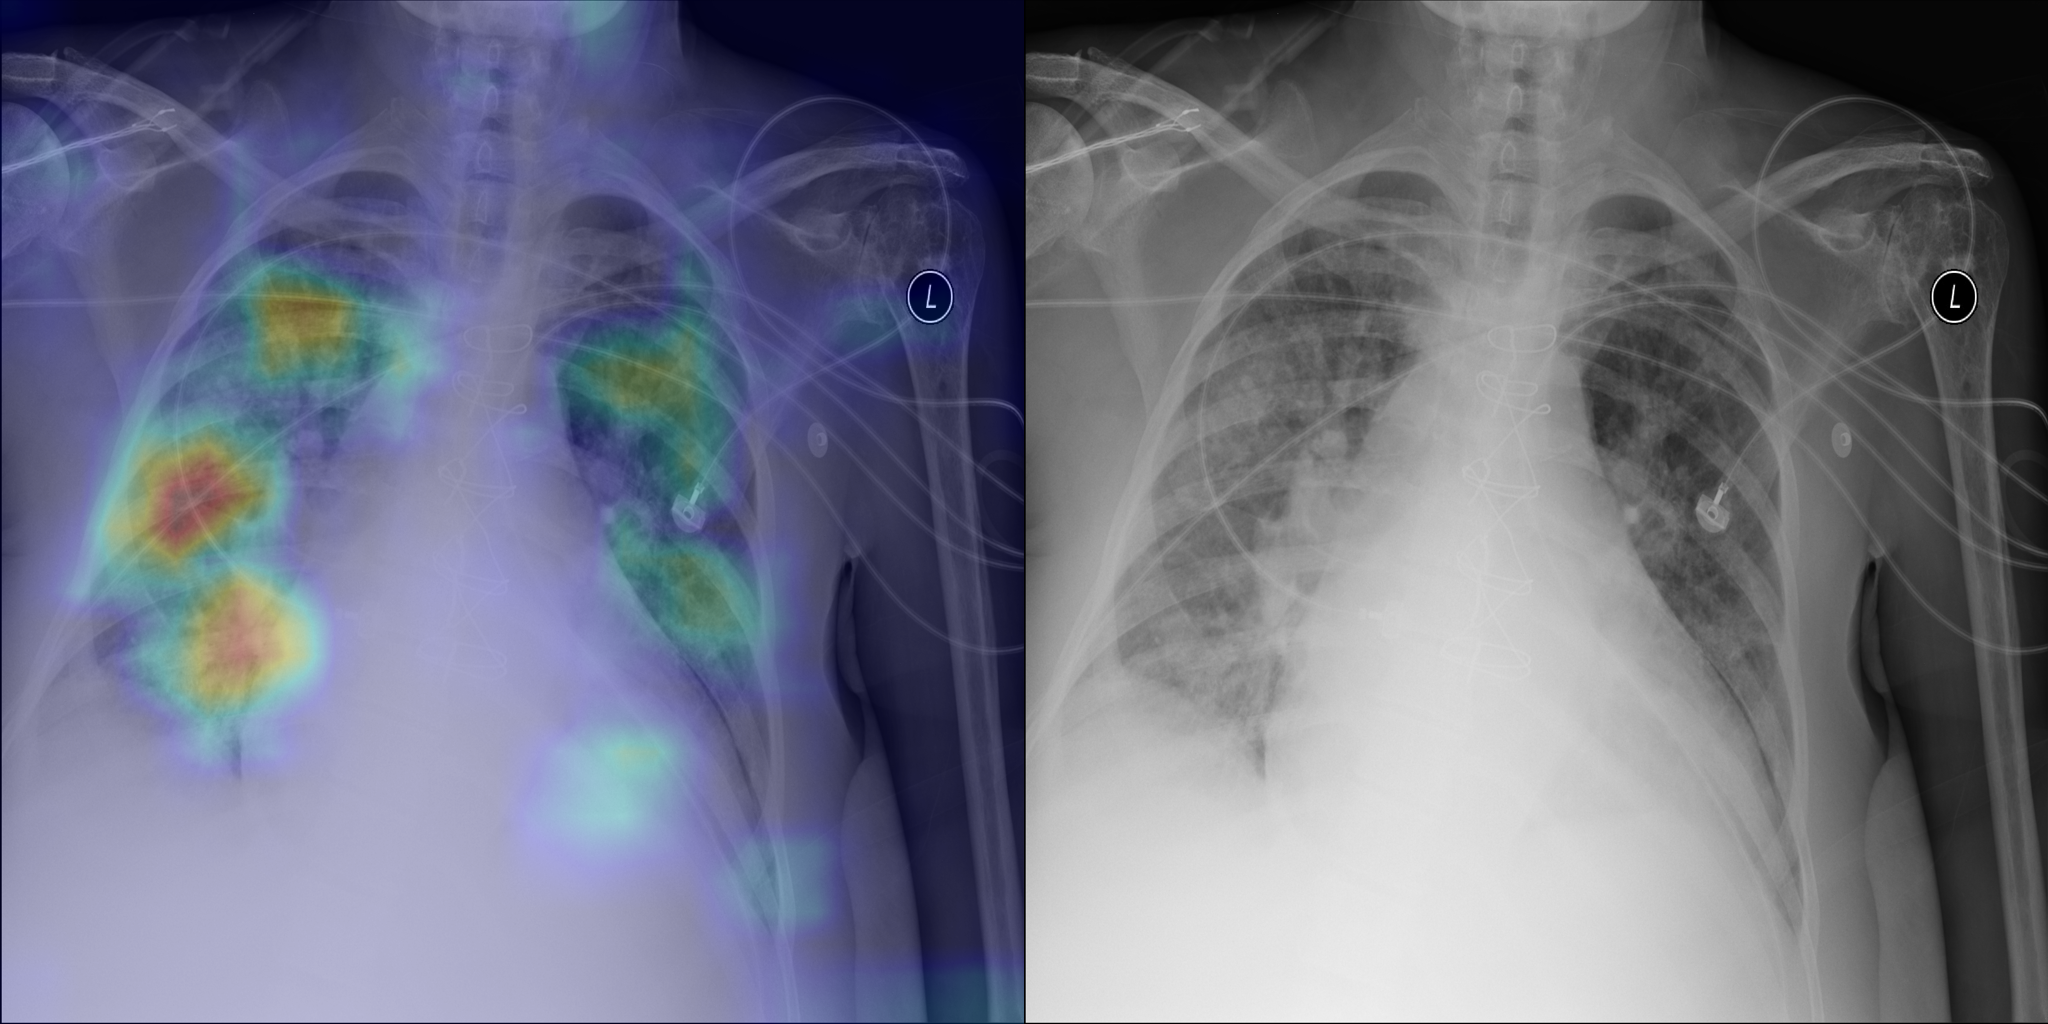
\includegraphics[width=1.0\textwidth]{Chapters/5. Conclusiones/img/Edema/1_1_00001373_031.png}
    \end{subfigure}
    \begin{subfigure}{0.4\textwidth}
        \centering
        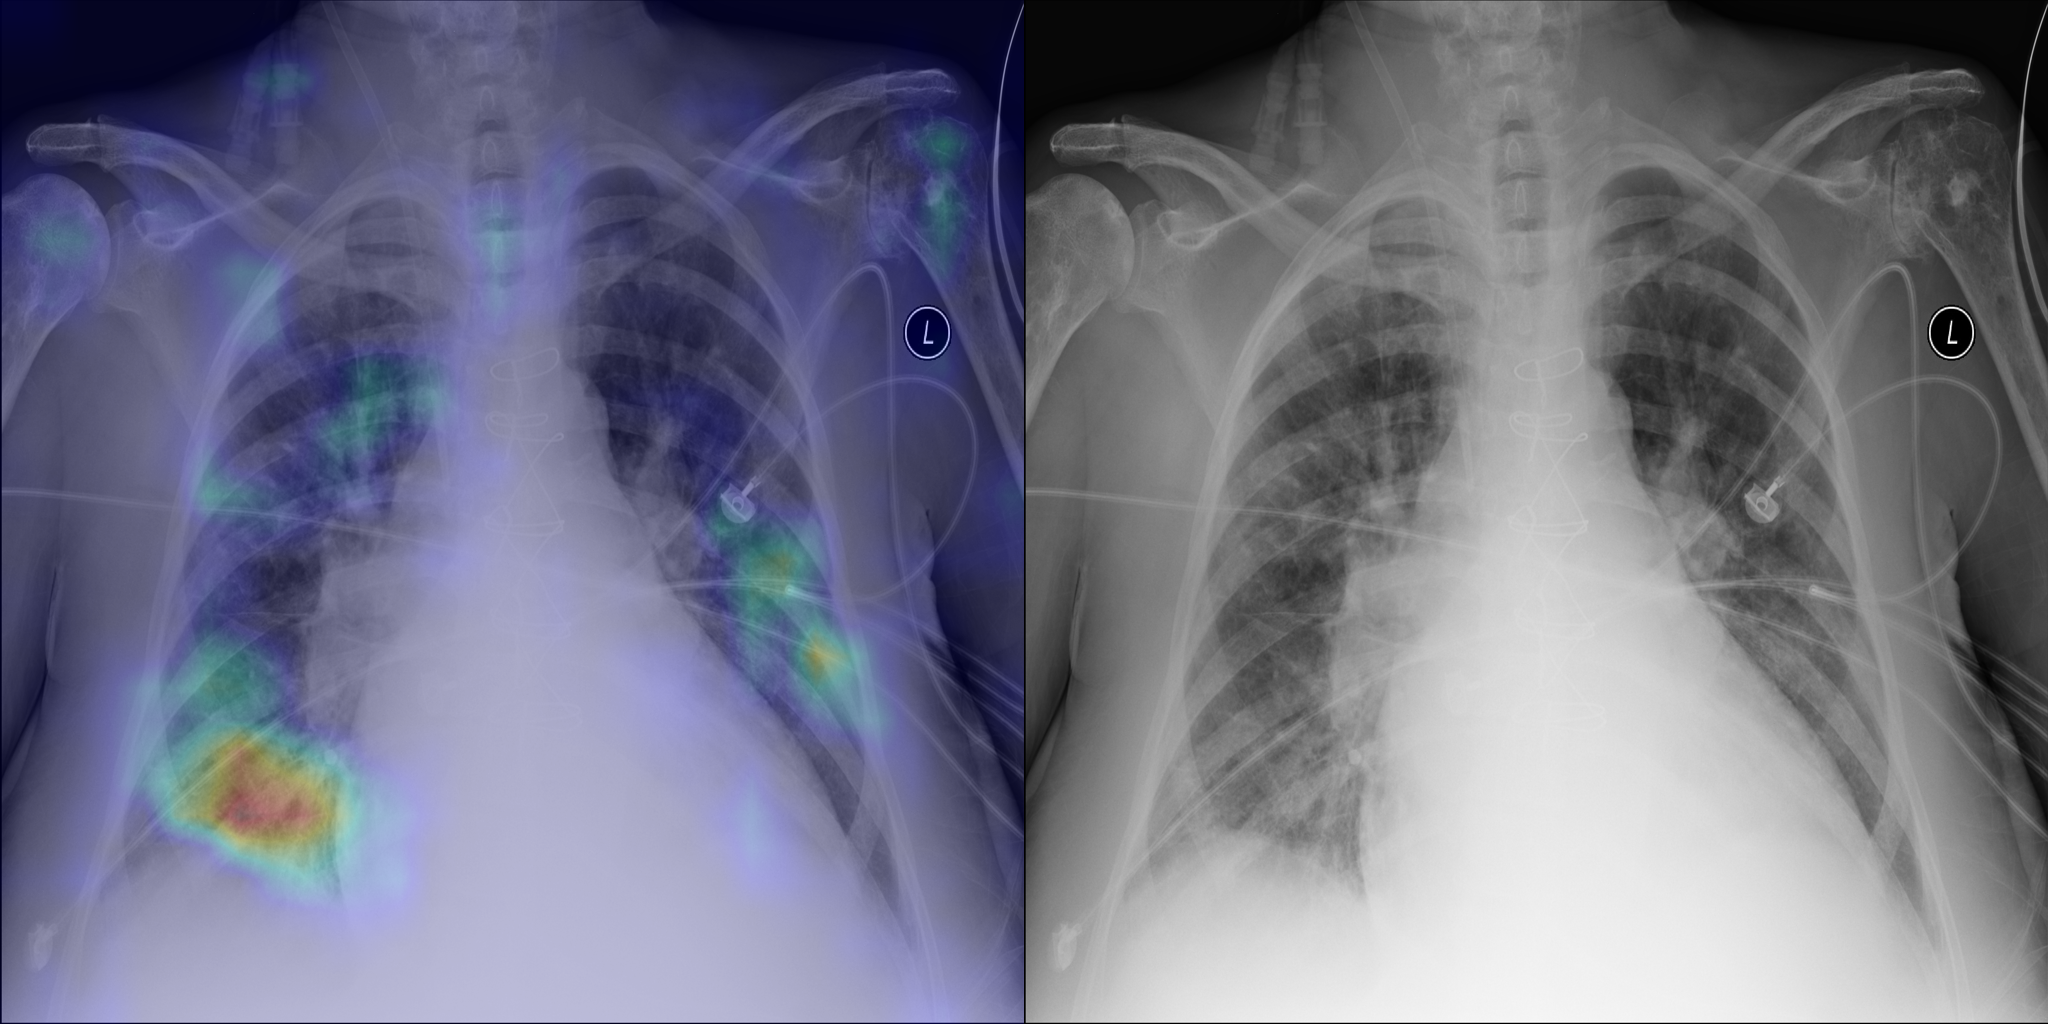
\includegraphics[width=1.0\textwidth]{Chapters/5. Conclusiones/img/Edema/1_1_00001373_032.png}
    \end{subfigure}
    \begin{subfigure}{0.4\textwidth}
        \centering
        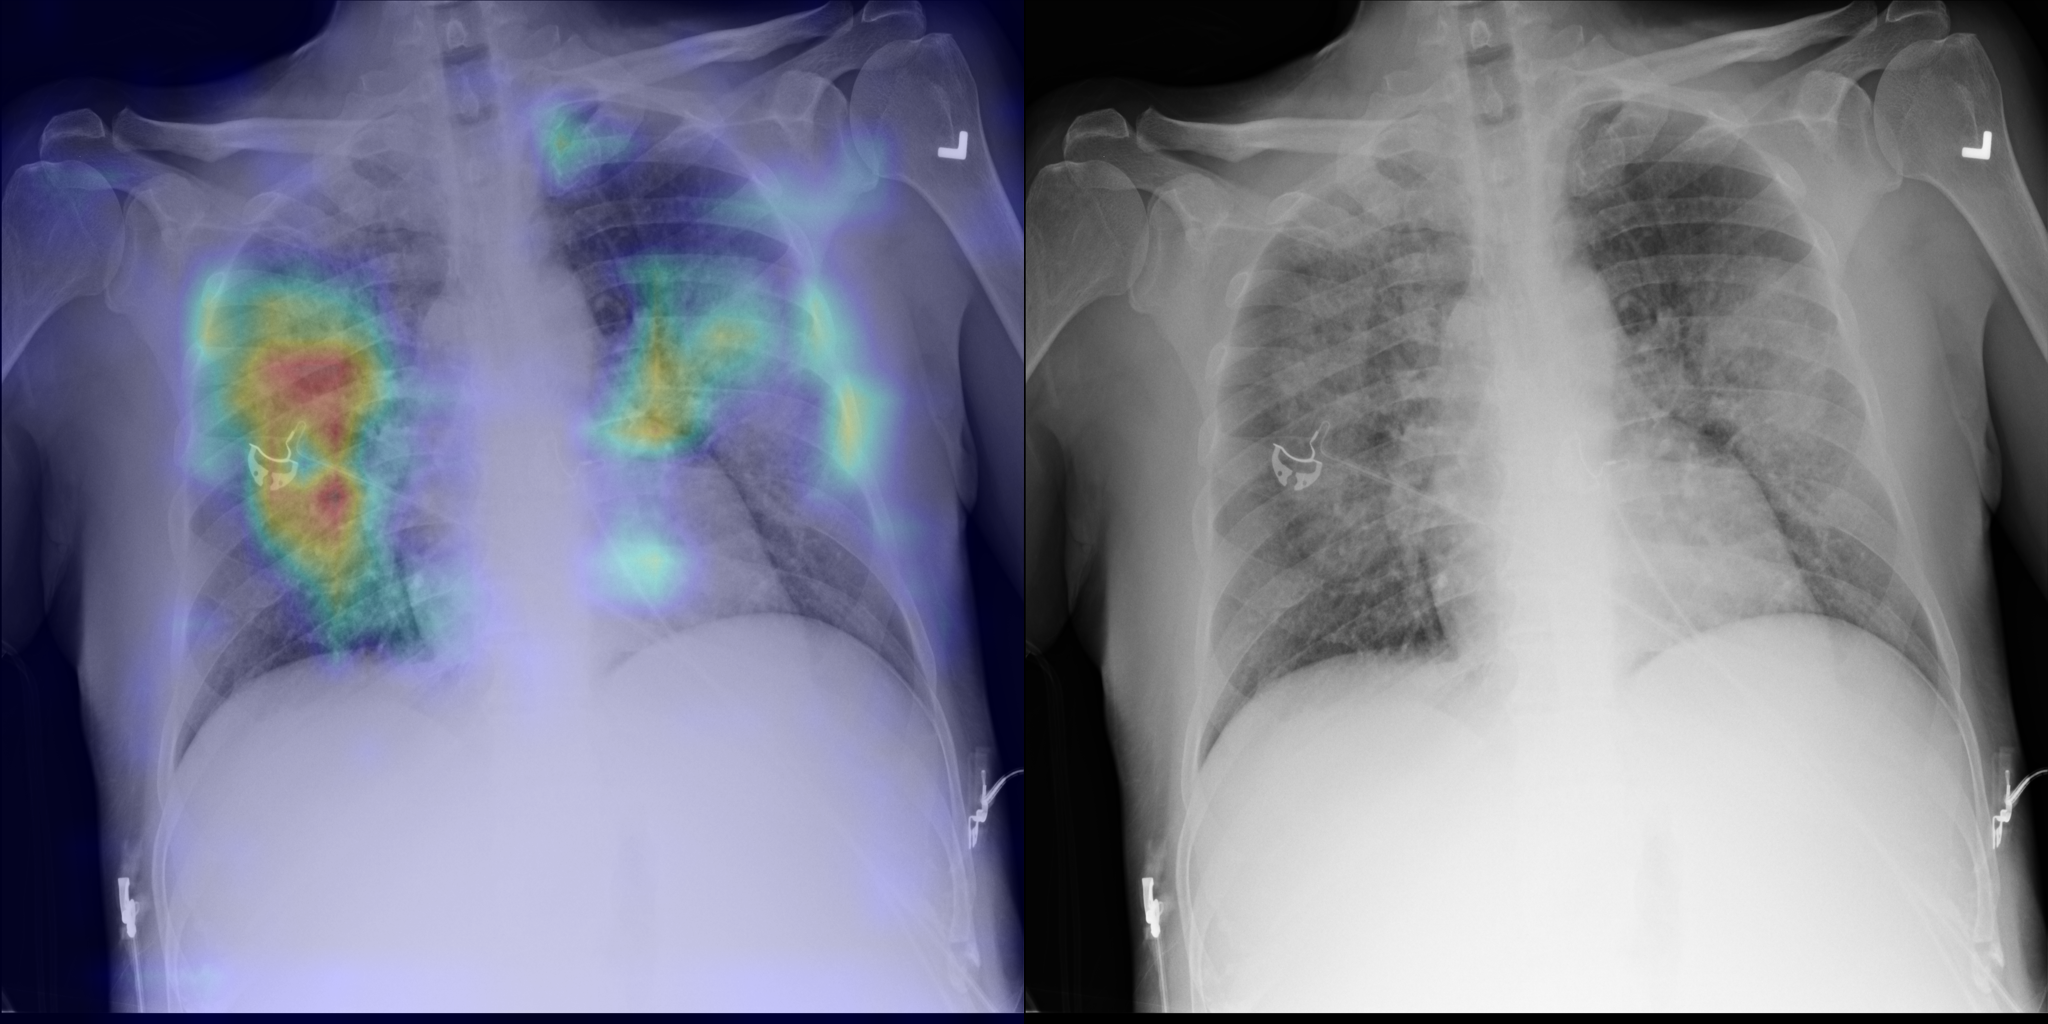
\includegraphics[width=1.0\textwidth]{Chapters/5. Conclusiones/img/Edema/1_1_00001787_000.png}
    \end{subfigure}
    \begin{subfigure}{0.4\textwidth}
        \centering
        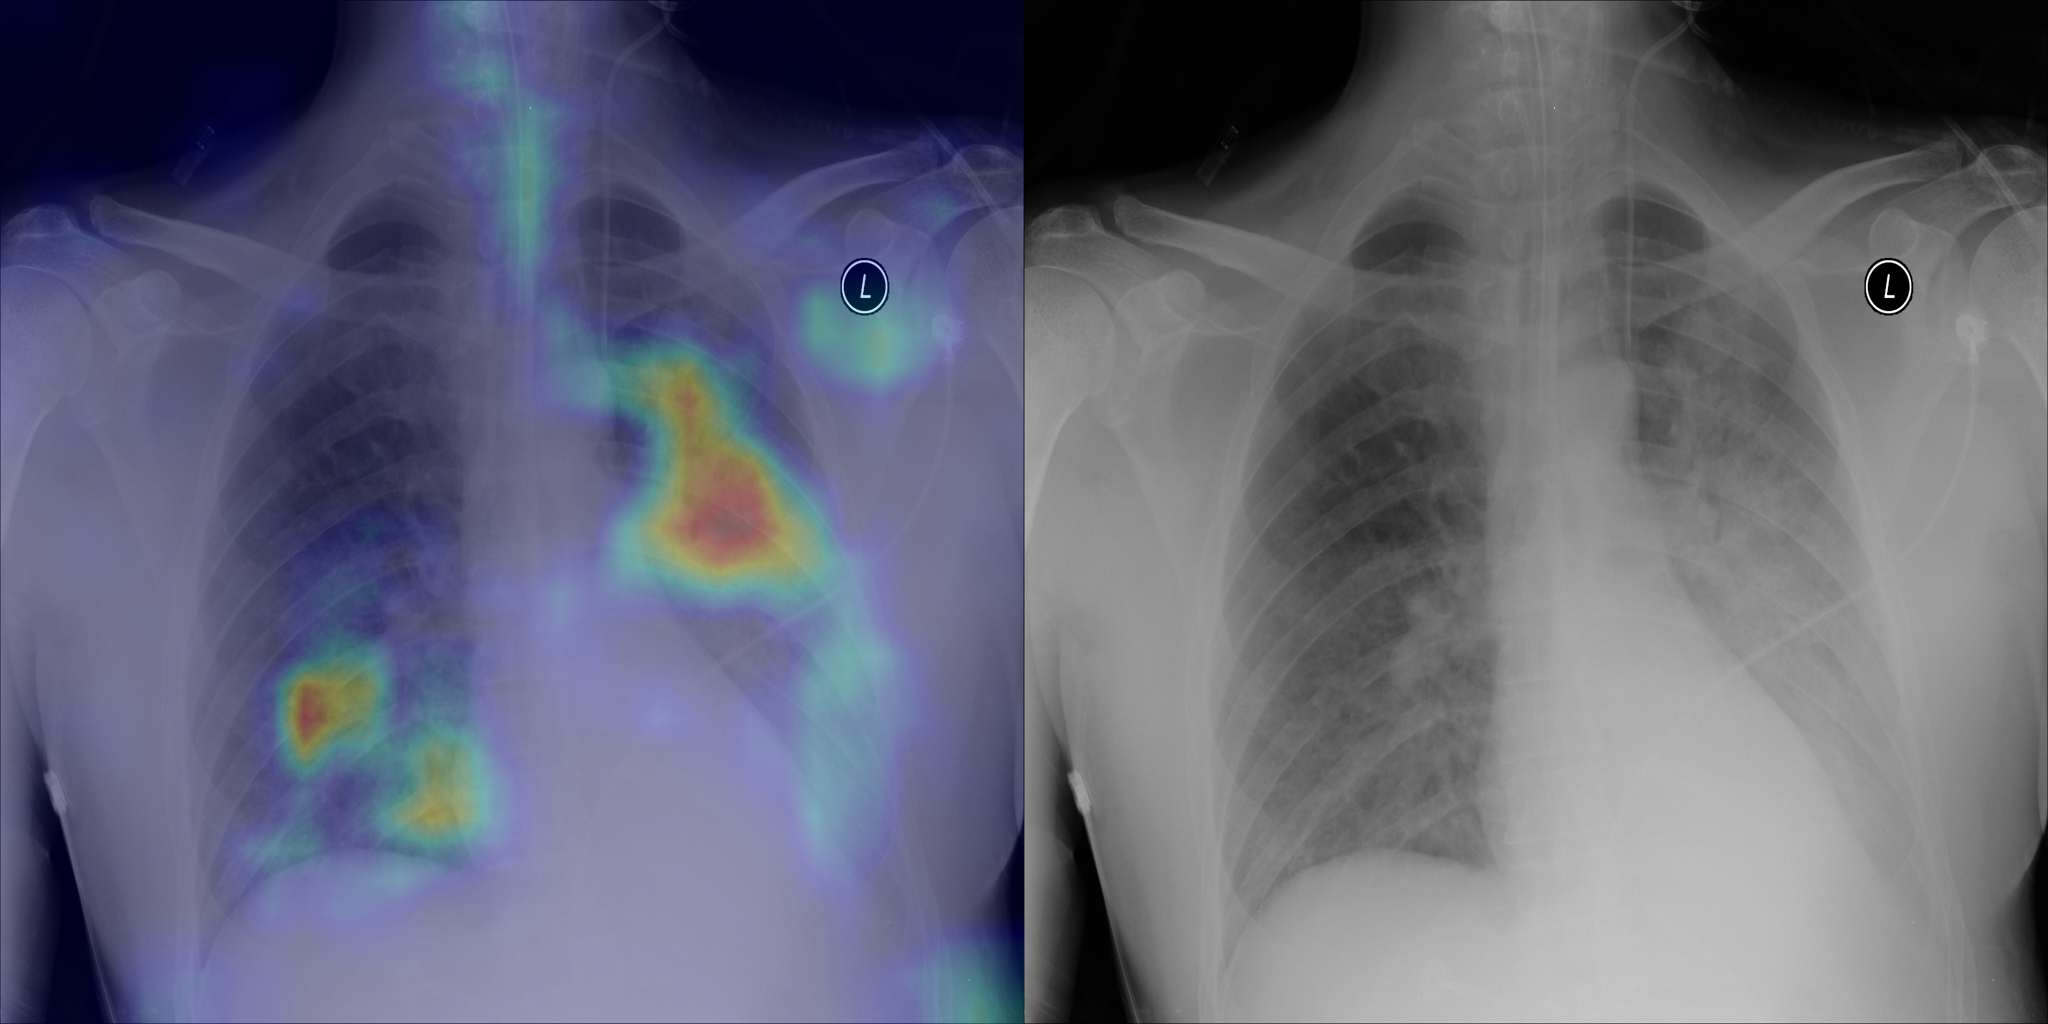
\includegraphics[width=1.0\textwidth]{Chapters/5. Conclusiones/img/Edema/1_1_00003528_021.png}
    \end{subfigure}
    \begin{subfigure}{0.4\textwidth}
        \centering
        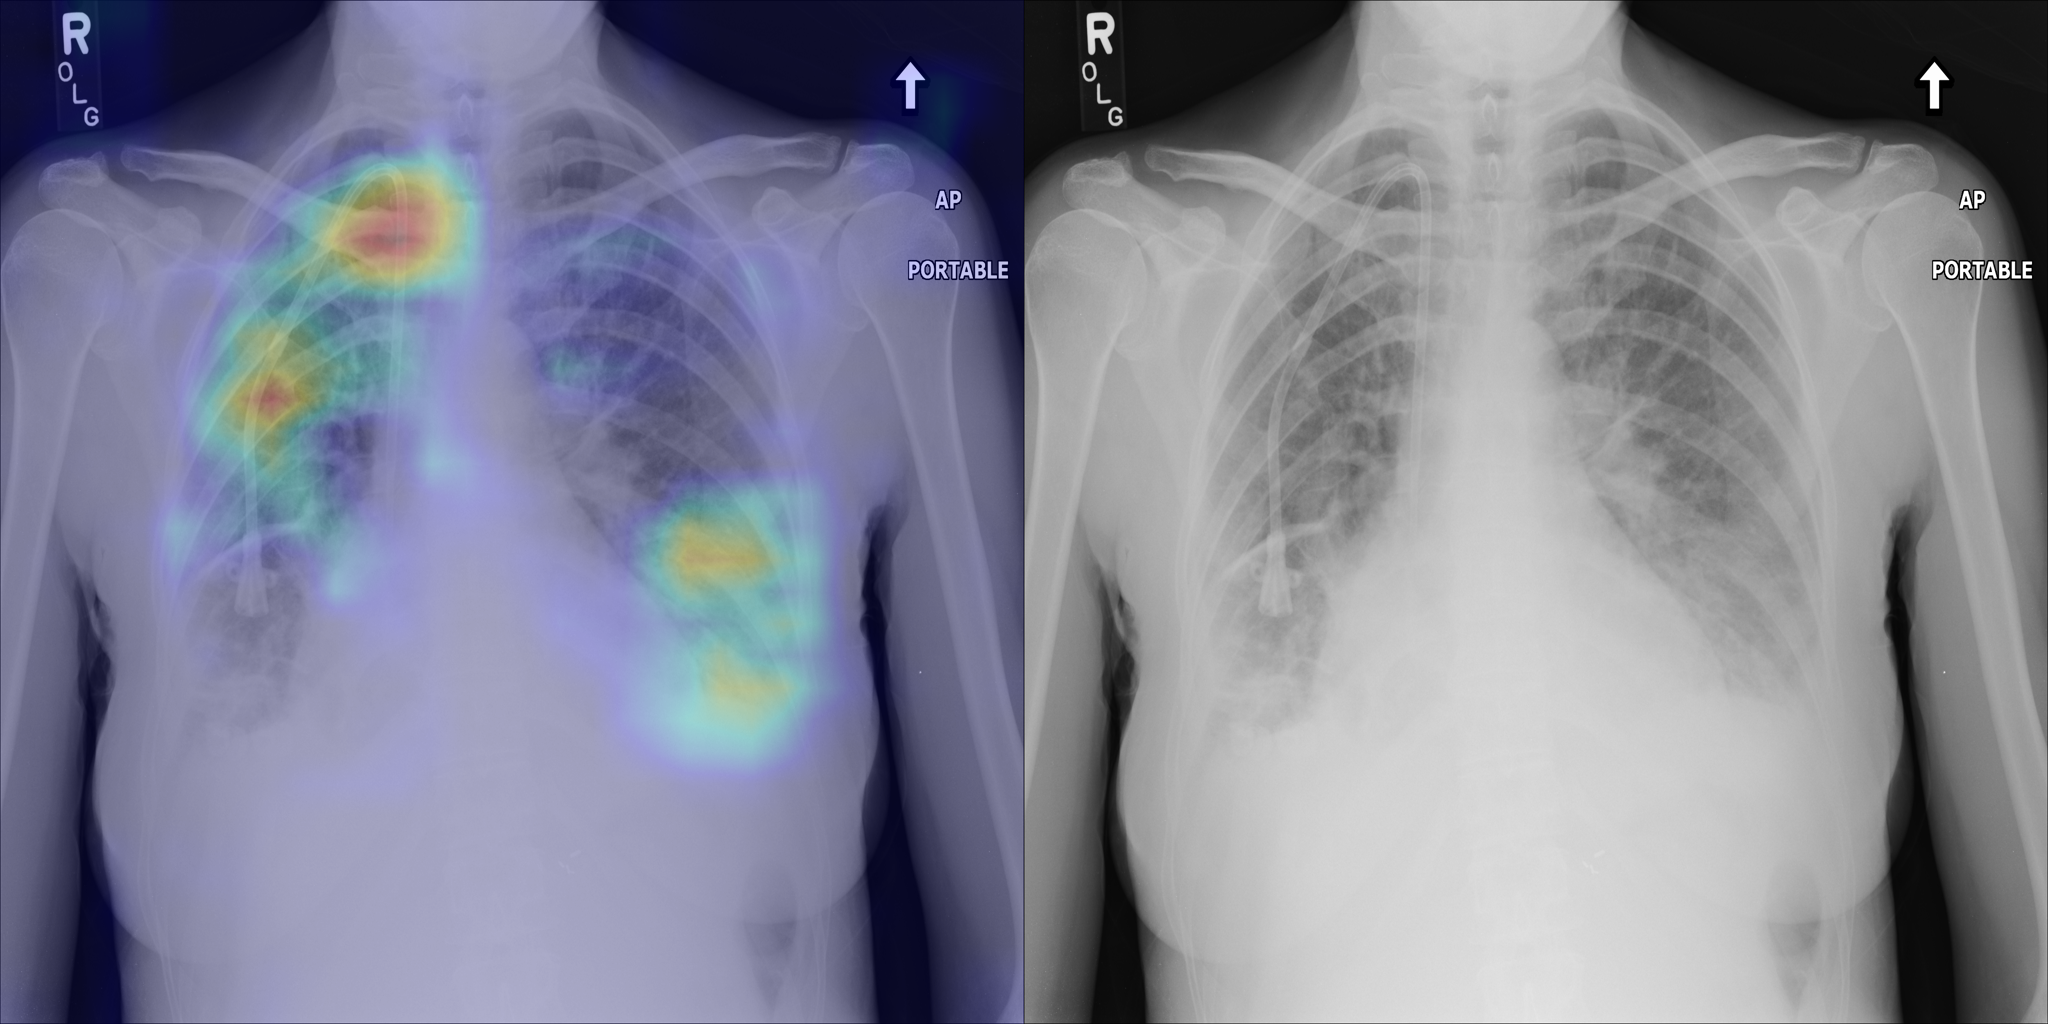
\includegraphics[width=1.0\textwidth]{Chapters/5. Conclusiones/img/Edema/1_1_00003803_009.png}
    \end{subfigure}
    \begin{subfigure}{0.4\textwidth}
        \centering
        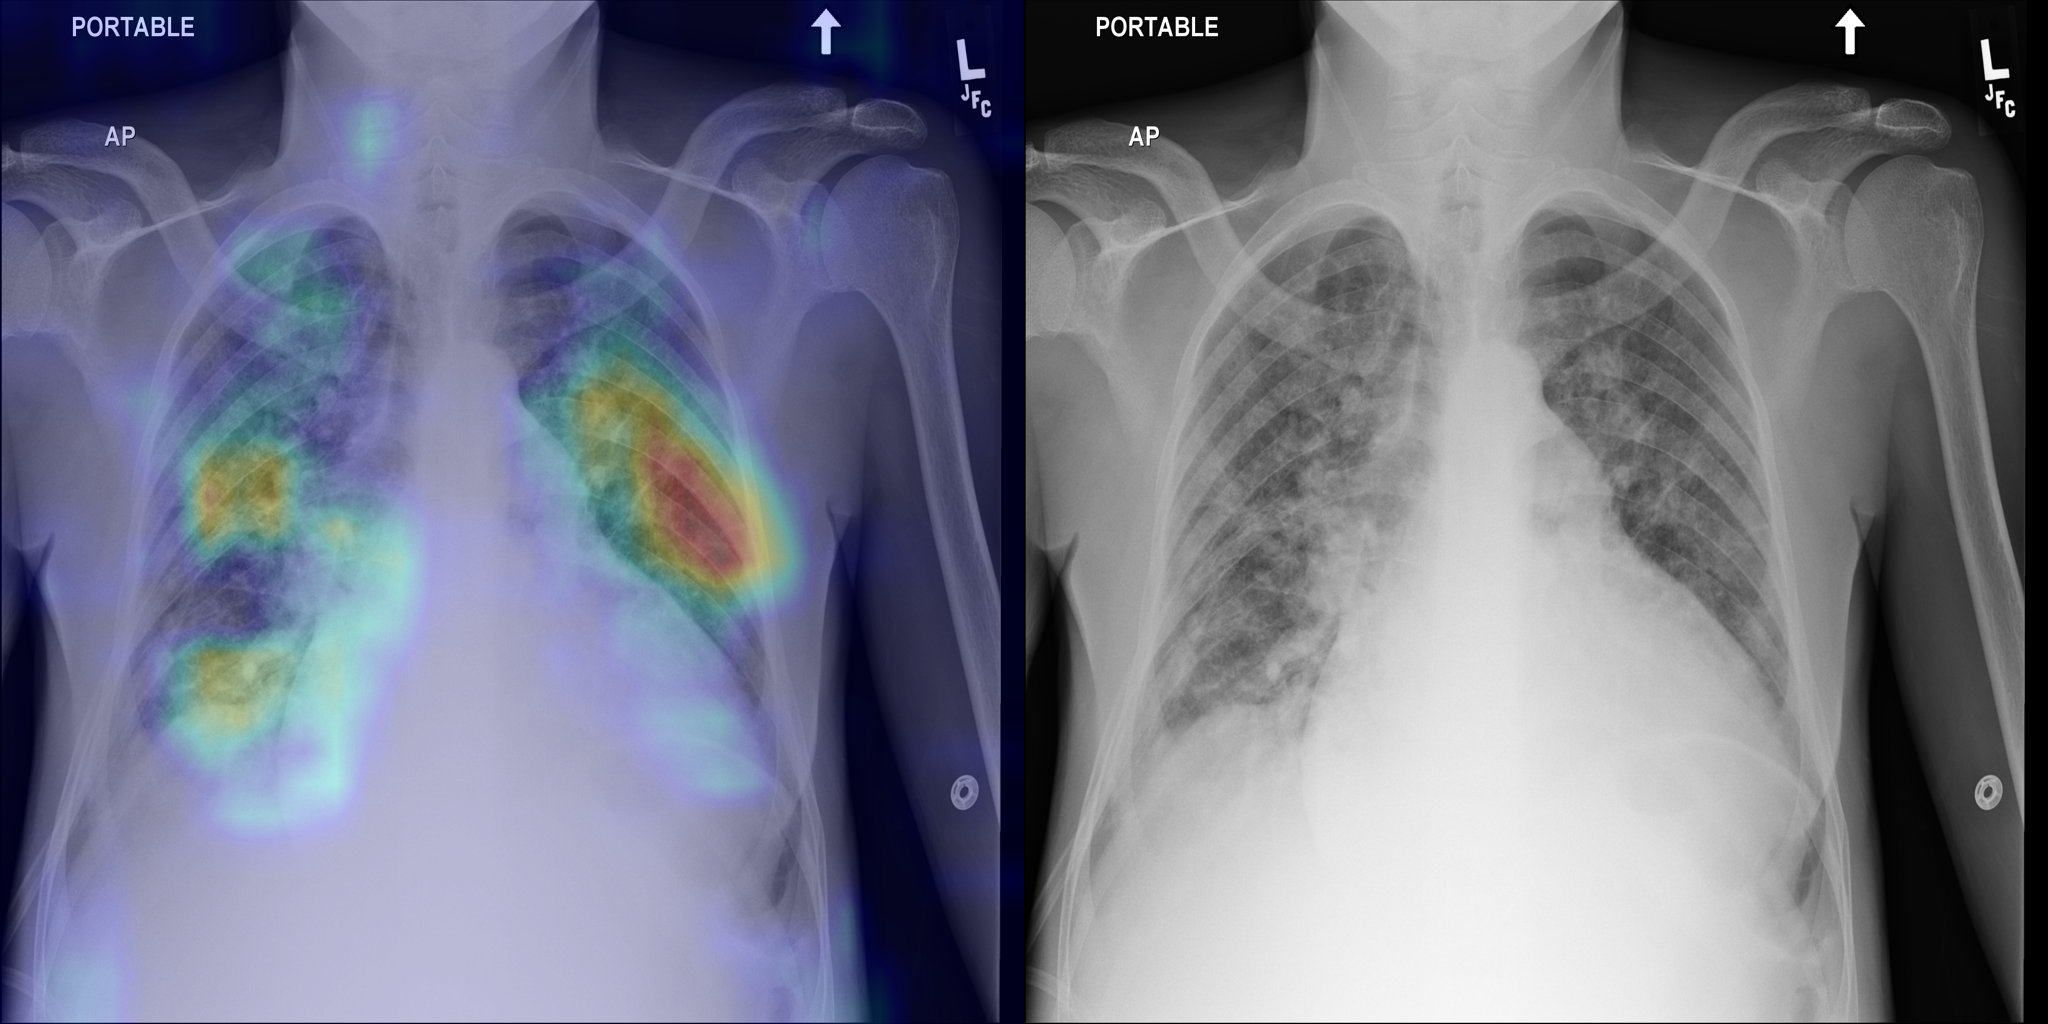
\includegraphics[width=1.0\textwidth]{Chapters/5. Conclusiones/img/Edema/1_1_00004533_020.png}
    \end{subfigure}
    \begin{subfigure}{0.4\textwidth}
        \centering
        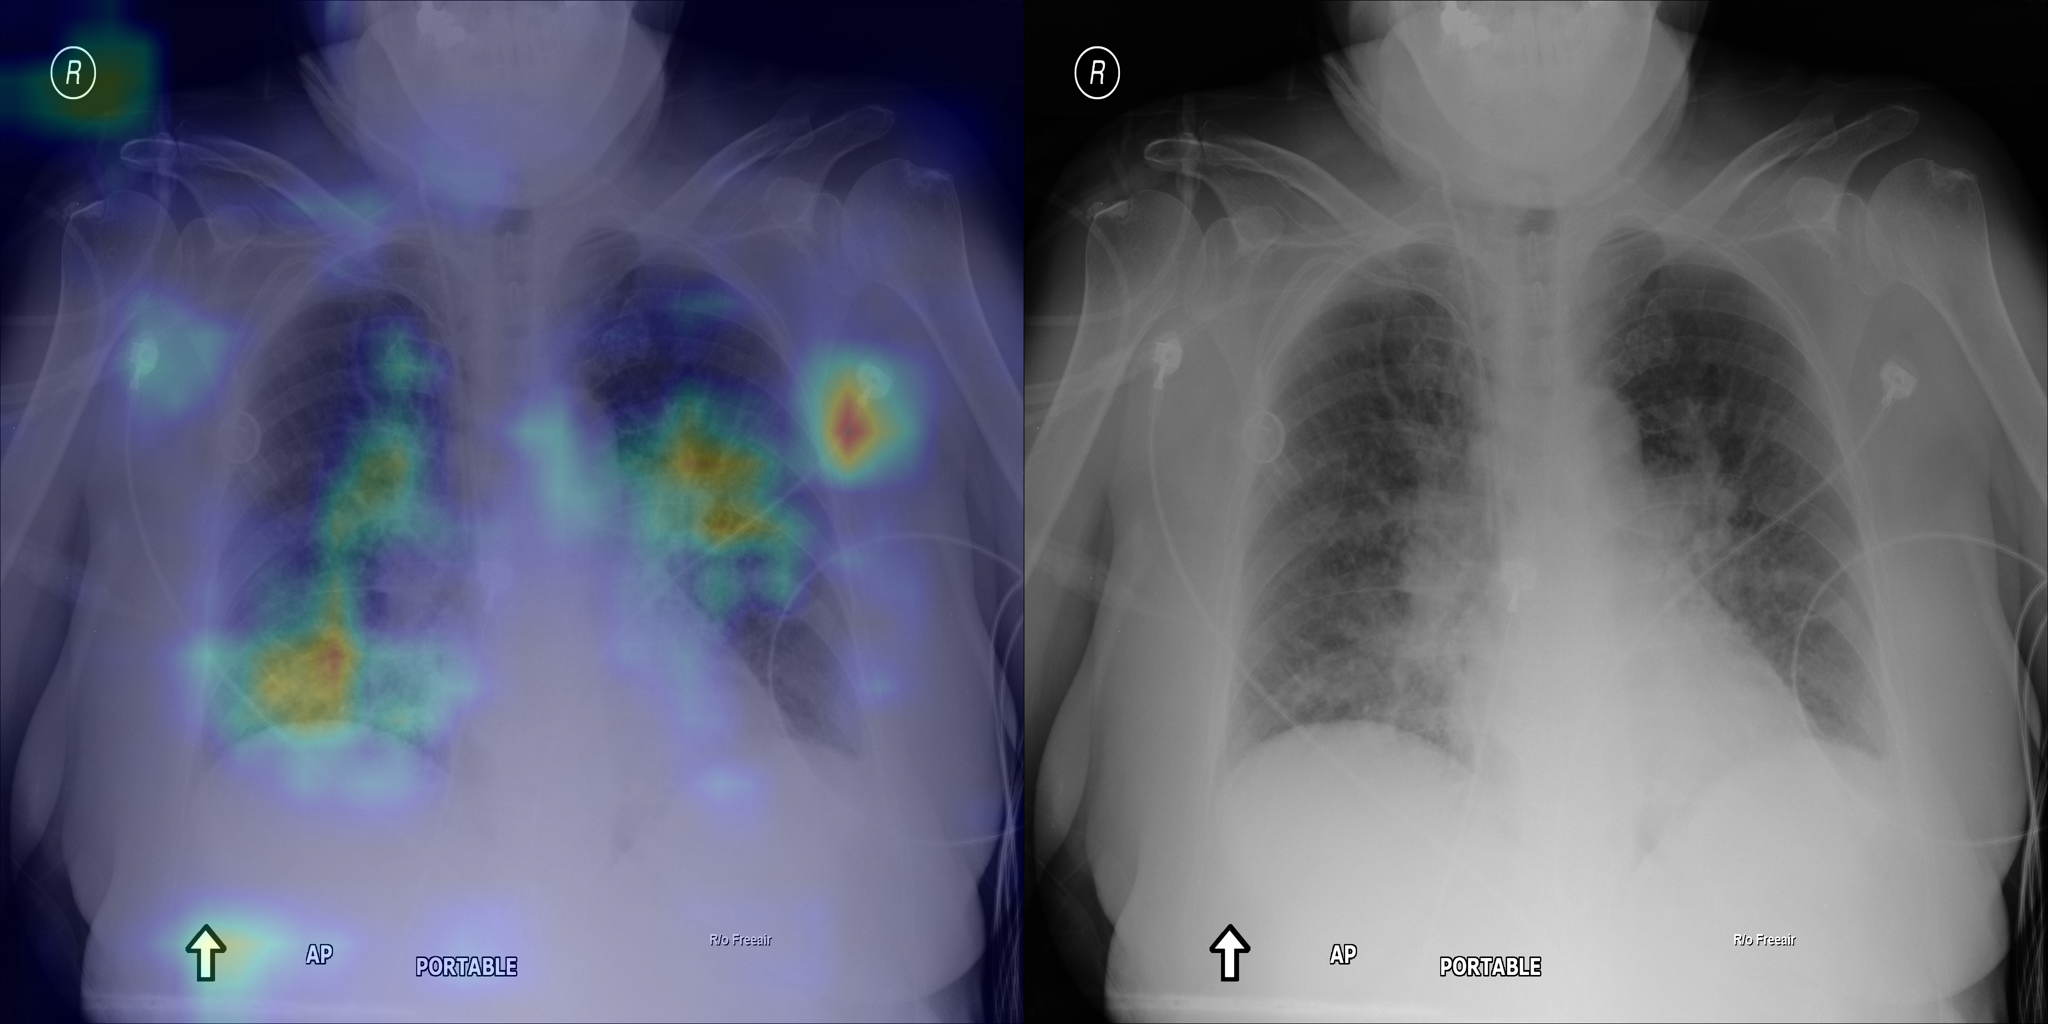
\includegraphics[width=1.0\textwidth]{Chapters/5. Conclusiones/img/Edema/1_1_00006304_002.png}
    \end{subfigure}
    \begin{subfigure}{0.4\textwidth}
        \centering
        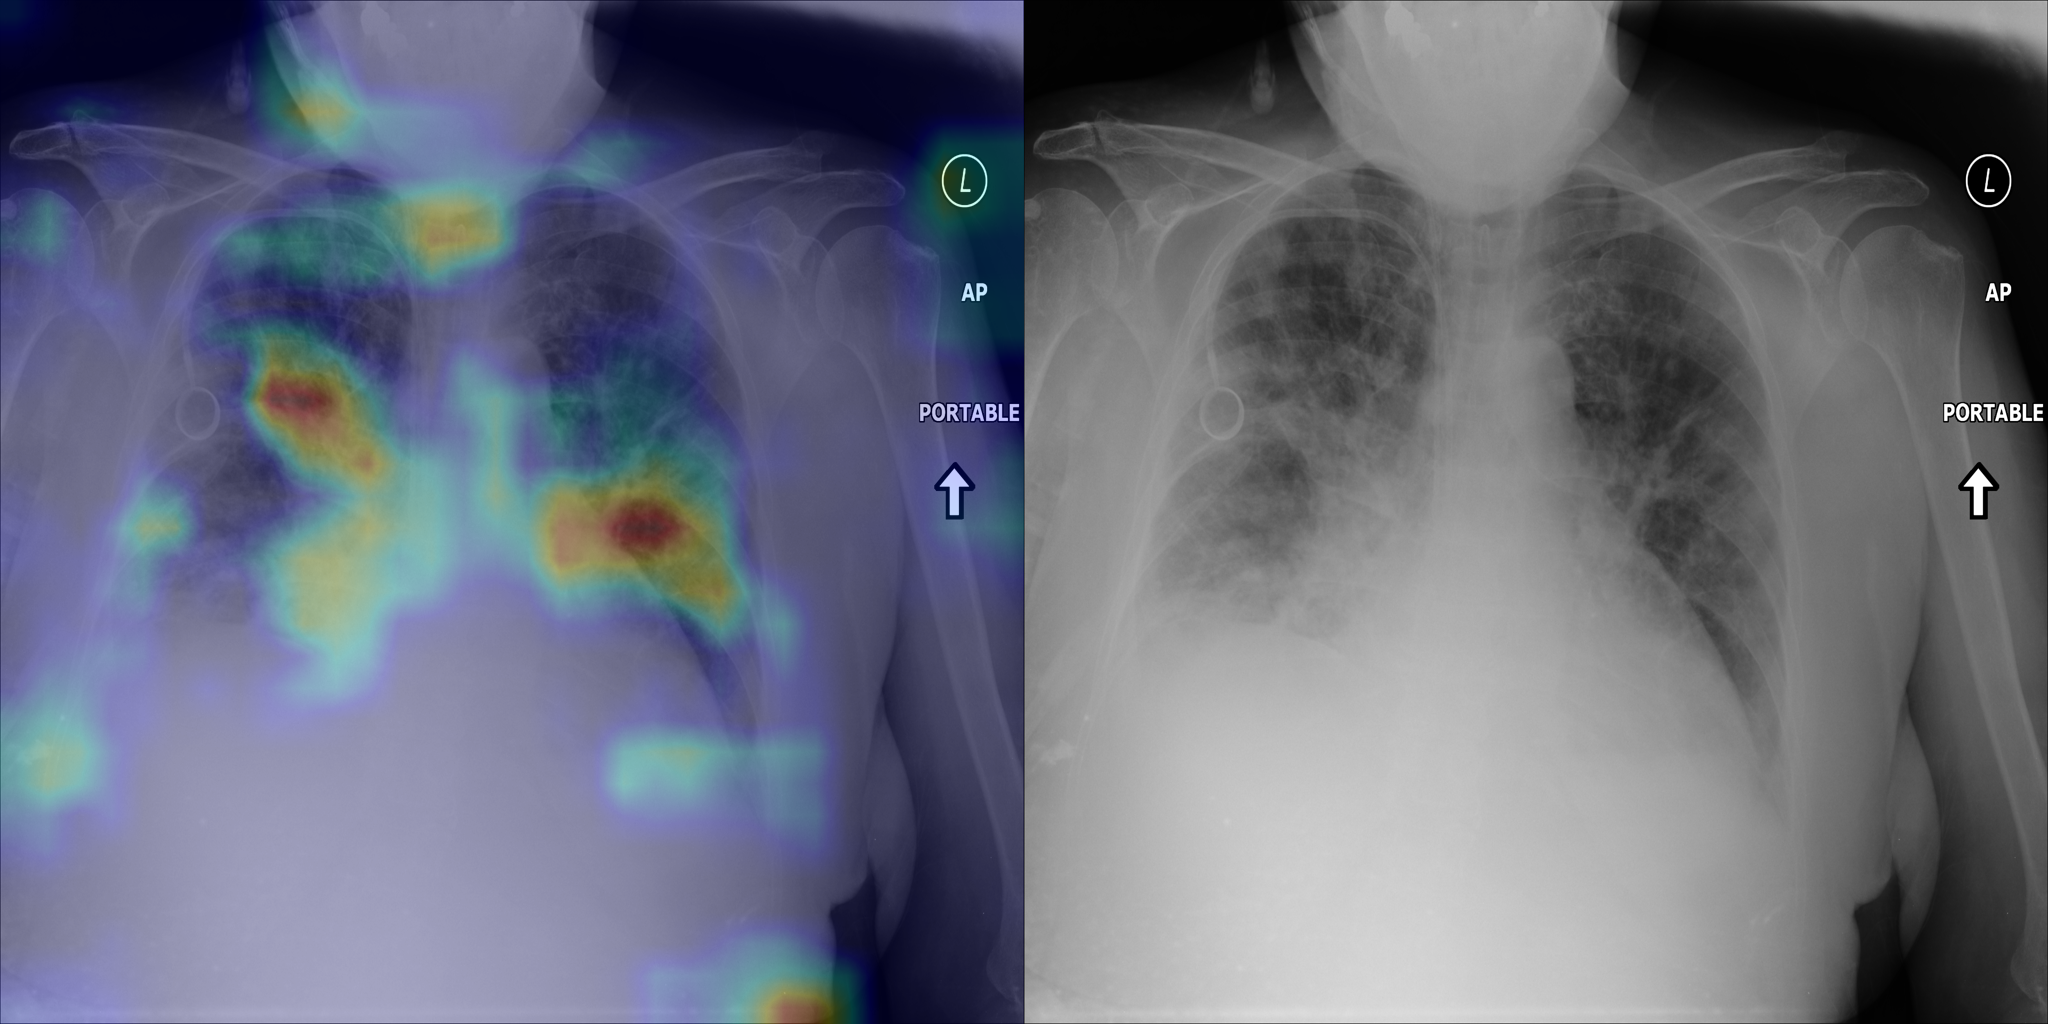
\includegraphics[width=1.0\textwidth]{Chapters/5. Conclusiones/img/Edema/1_1_00006304_006.png}
    \end{subfigure}
    \begin{subfigure}{0.4\textwidth}
        \centering
        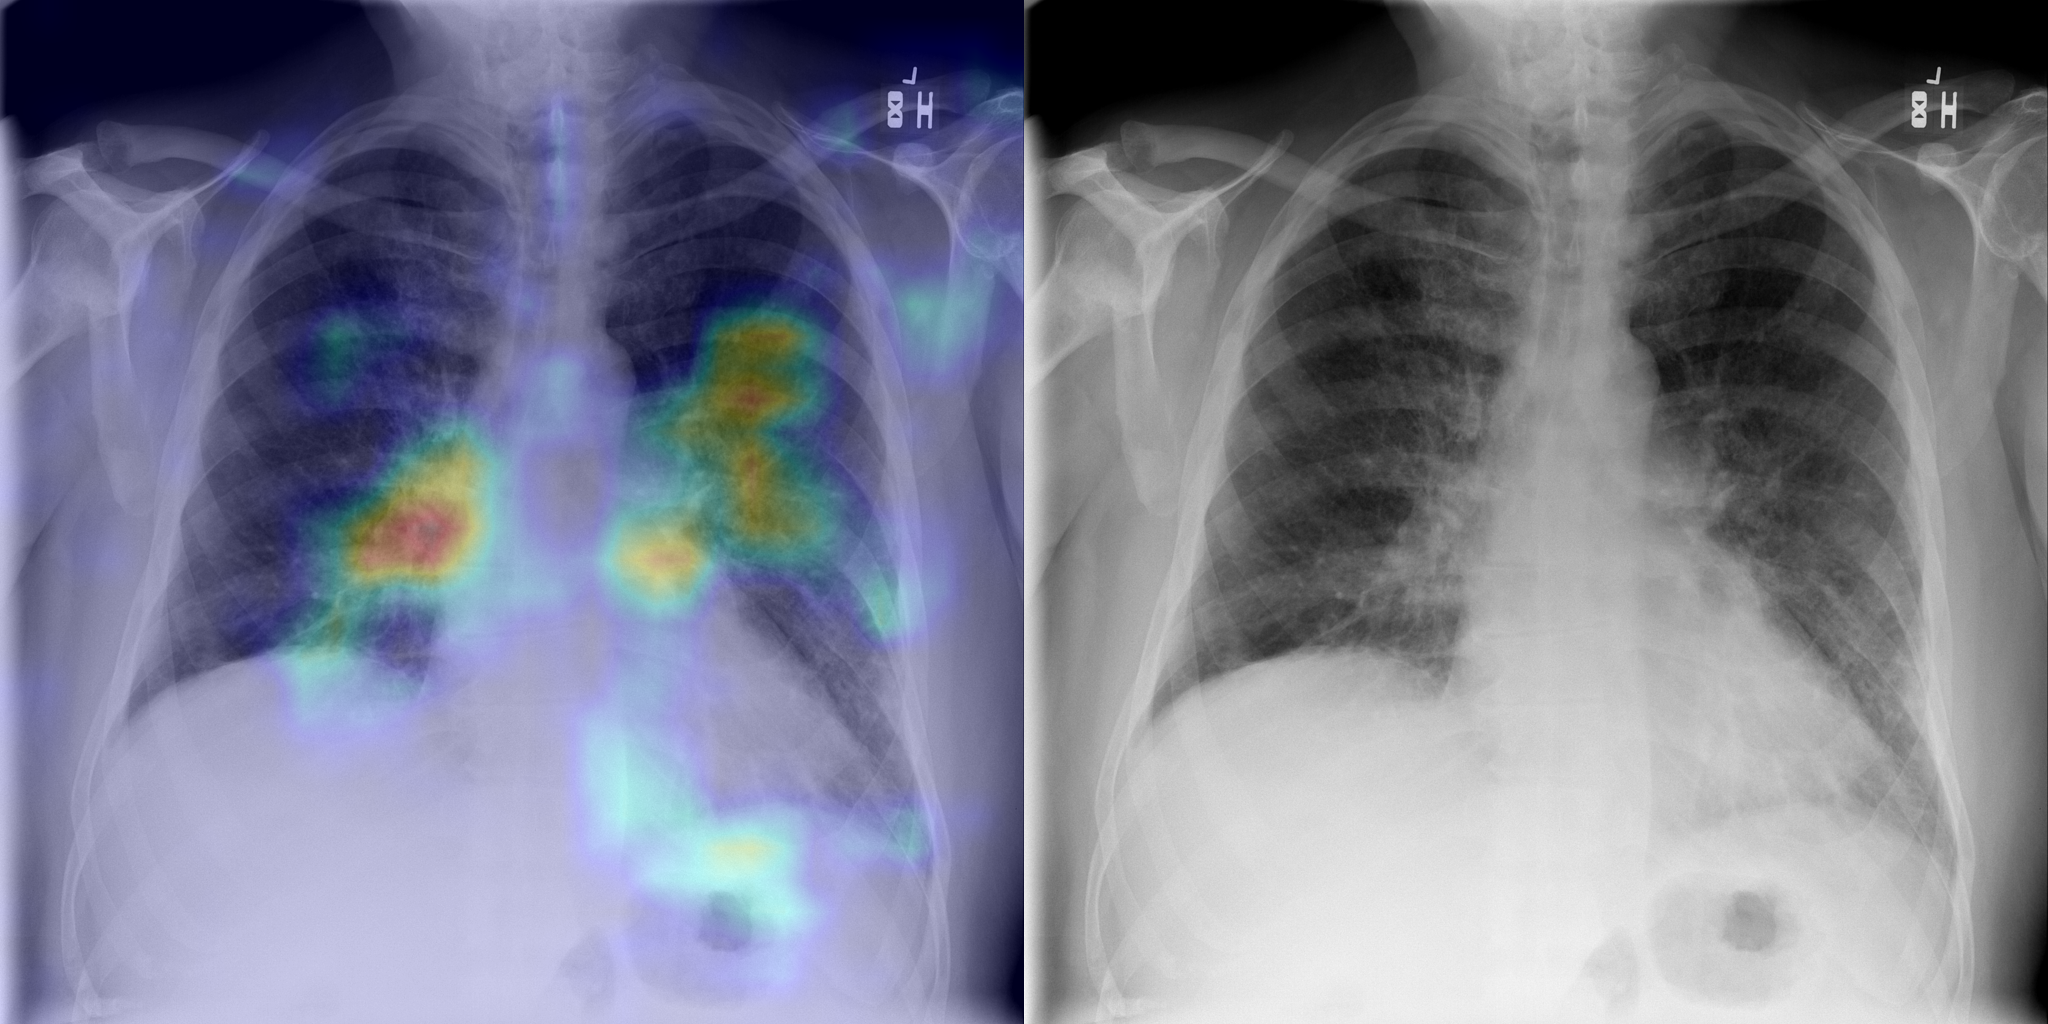
\includegraphics[width=1.0\textwidth]{Chapters/5. Conclusiones/img/Edema/1_1_00010535_002.png}
    \end{subfigure}
    \begin{subfigure}{0.4\textwidth}
        \centering
        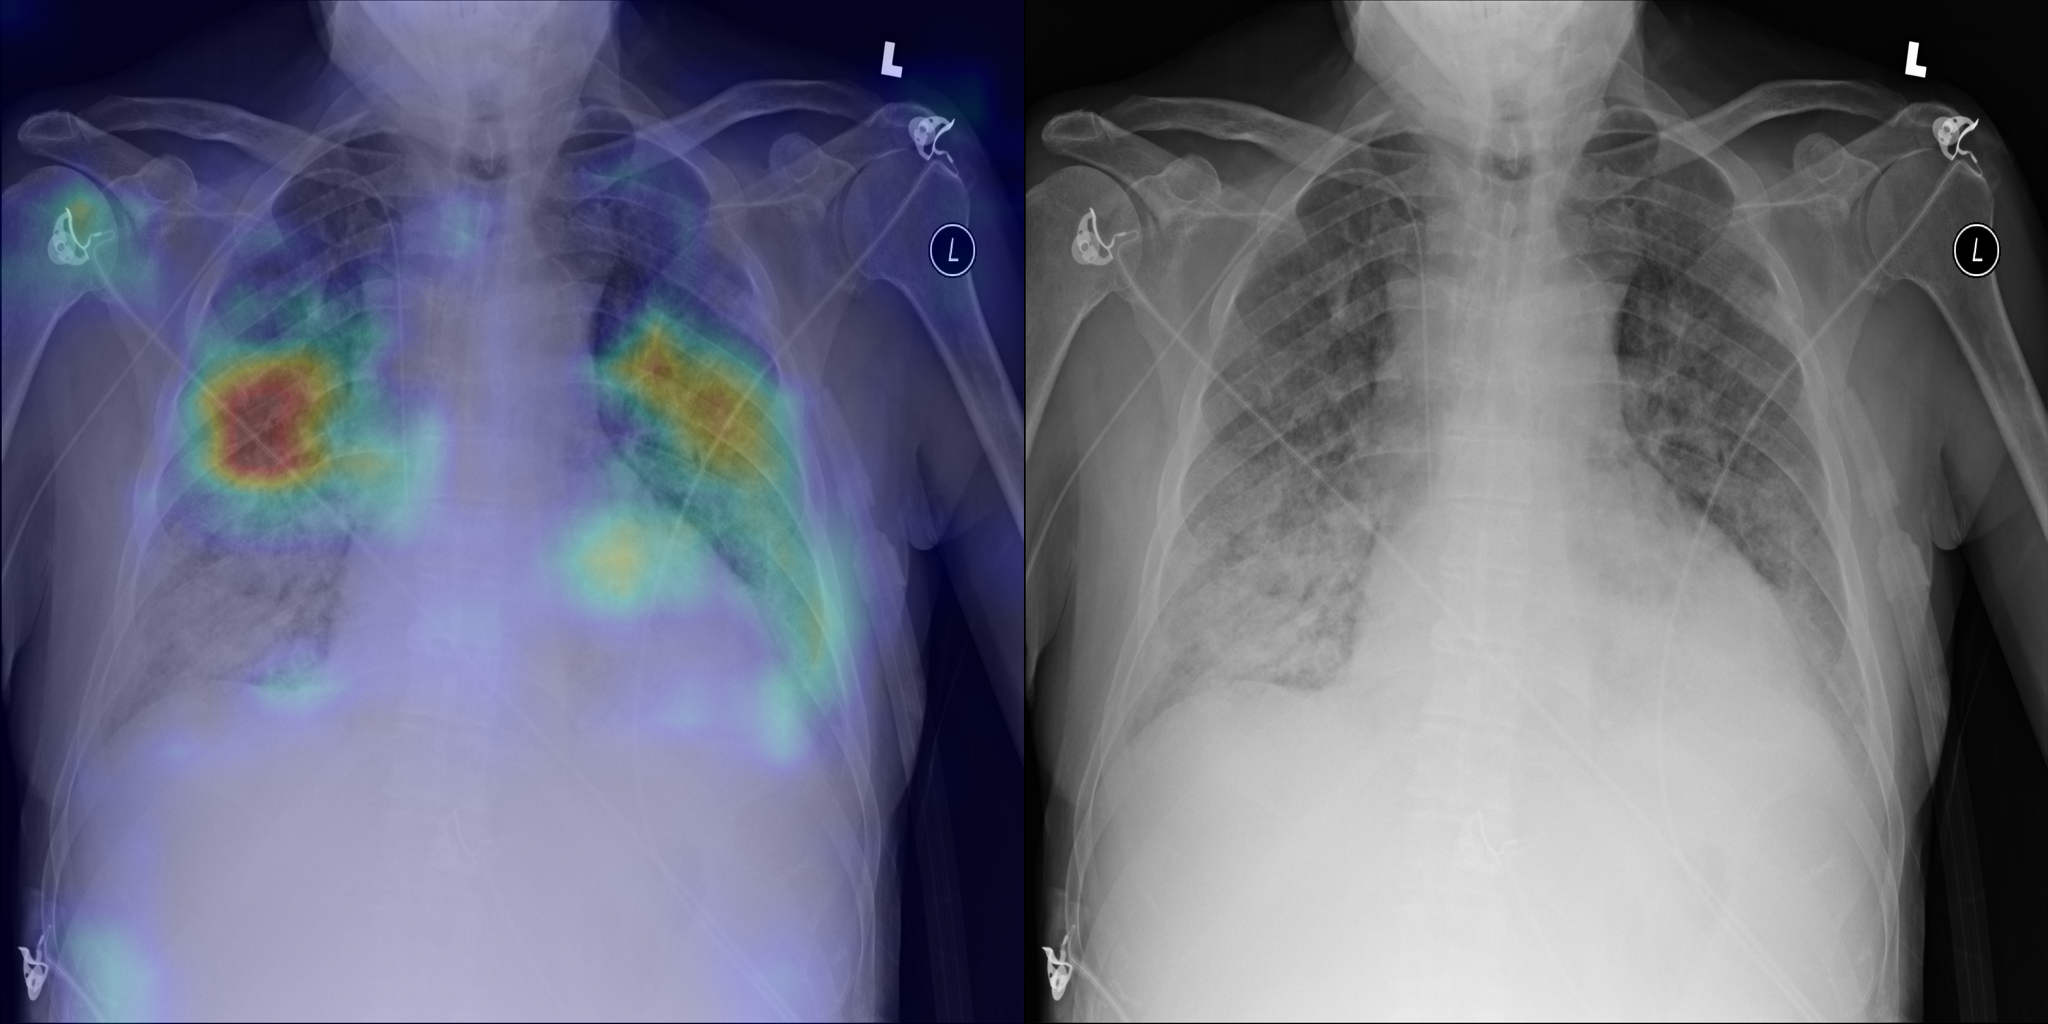
\includegraphics[width=1.0\textwidth]{Chapters/5. Conclusiones/img/Edema/1_1_00011583_006.png}
    \end{subfigure}

    \caption[short]{Edema. Radiografías detectadas con la patología de edema pulmonar por los
                    radiólogos. A la izquierda de cada imagen el GradCam correspondiente a la detección
                    de la patología como positivo por el modelo CNN.}
\end{figure}

\begin{figure}[b]
    \centering
    \begin{subfigure}{0.4\textwidth}
        \centering
        \includegraphics[width=1.0\textwidth]{Chapters/5. Conclusiones/img/Effusion/1_1_00000092_001.png}
    \end{subfigure}
    \begin{subfigure}{0.4\textwidth}
        \centering
        \includegraphics[width=1.0\textwidth]{Chapters/5. Conclusiones/img/Effusion/1_1_00000147_002.png}
    \end{subfigure}
    \begin{subfigure}{0.4\textwidth}
        \centering
        \includegraphics[width=1.0\textwidth]{Chapters/5. Conclusiones/img/Effusion/1_1_00000181_005.png}
    \end{subfigure}
    \begin{subfigure}{0.4\textwidth}
        \centering
        \includegraphics[width=1.0\textwidth]{Chapters/5. Conclusiones/img/Effusion/1_1_00000181_054.png}
    \end{subfigure}
    \begin{subfigure}{0.4\textwidth}
        \centering
        \includegraphics[width=1.0\textwidth]{Chapters/5. Conclusiones/img/Effusion/1_1_00000181_055.png}
    \end{subfigure}
    \begin{subfigure}{0.4\textwidth}
        \centering
        \includegraphics[width=1.0\textwidth]{Chapters/5. Conclusiones/img/Effusion/1_1_00000211_004.png}
    \end{subfigure}
    \begin{subfigure}{0.4\textwidth}
        \centering
        \includegraphics[width=1.0\textwidth]{Chapters/5. Conclusiones/img/Effusion/1_1_00000211_008.png}
    \end{subfigure}
    \begin{subfigure}{0.4\textwidth}
        \centering
        \includegraphics[width=1.0\textwidth]{Chapters/5. Conclusiones/img/Effusion/1_1_00000211_011.png}
    \end{subfigure}
    \begin{subfigure}{0.4\textwidth}
        \centering
        \includegraphics[width=1.0\textwidth]{Chapters/5. Conclusiones/img/Effusion/1_1_00022883_011.png}
    \end{subfigure}
    \begin{subfigure}{0.4\textwidth}
        \centering
        \includegraphics[width=1.0\textwidth]{Chapters/5. Conclusiones/img/Effusion/1_1_00022899_009.png}
    \end{subfigure}

    \caption[short]{Derrame pleural. Radiografías detectadas con la patología de derrame pleural por los
                    radiólogos. A la izquierda de cada imagen el GradCam correspondiente a la detección
                    de la patología como positivo por el modelo CNN.}
\end{figure}

\begin{figure}[b]
    \centering
    \begin{subfigure}{0.4\textwidth}
        \centering
        \includegraphics[width=1.0\textwidth]{Chapters/5. Conclusiones/img/Emphysema/1_1_00000312_001.png}
    \end{subfigure}
    \begin{subfigure}{0.4\textwidth}
        \centering
        \includegraphics[width=1.0\textwidth]{Chapters/5. Conclusiones/img/Emphysema/1_1_00000732_006.png}
    \end{subfigure}
    \begin{subfigure}{0.4\textwidth}
        \centering
        \includegraphics[width=1.0\textwidth]{Chapters/5. Conclusiones/img/Emphysema/1_1_00001093_000.png}
    \end{subfigure}
    \begin{subfigure}{0.4\textwidth}
        \centering
        \includegraphics[width=1.0\textwidth]{Chapters/5. Conclusiones/img/Emphysema/1_1_00001555_000.png}
    \end{subfigure}
    \begin{subfigure}{0.4\textwidth}
        \centering
        \includegraphics[width=1.0\textwidth]{Chapters/5. Conclusiones/img/Emphysema/1_1_00008841_062.png}
    \end{subfigure}
    \begin{subfigure}{0.4\textwidth}
        \centering
        \includegraphics[width=1.0\textwidth]{Chapters/5. Conclusiones/img/Emphysema/1_1_00011683_042.png}
    \end{subfigure}
    \begin{subfigure}{0.4\textwidth}
        \centering
        \includegraphics[width=1.0\textwidth]{Chapters/5. Conclusiones/img/Emphysema/1_1_00012298_007.png}
    \end{subfigure}
    \begin{subfigure}{0.4\textwidth}
        \centering
        \includegraphics[width=1.0\textwidth]{Chapters/5. Conclusiones/img/Emphysema/1_1_00015387_000.png}
    \end{subfigure}
    \begin{subfigure}{0.4\textwidth}
        \centering
        \includegraphics[width=1.0\textwidth]{Chapters/5. Conclusiones/img/Emphysema/1_1_00023075_007.png}
    \end{subfigure}
    \begin{subfigure}{0.4\textwidth}
        \centering
        \includegraphics[width=1.0\textwidth]{Chapters/5. Conclusiones/img/Emphysema/1_1_00023078_006.png}
    \end{subfigure}

    \caption[short]{Enfisema pulmonar. Radiografías detectadas con la patología de enfisema pulmonar por los
                    radiólogos. A la izquierda de cada imagen el GradCam correspondiente a la detección
                    de la patología como positivo por el modelo CNN.}
\end{figure}

\begin{figure}[b]
    \centering
    \begin{subfigure}{0.4\textwidth}
        \centering
        \includegraphics[width=1.0\textwidth]{Chapters/5. Conclusiones/img/Fibrosis/1_1_00000092_003.png}
    \end{subfigure}
    \begin{subfigure}{0.4\textwidth}
        \centering
        \includegraphics[width=1.0\textwidth]{Chapters/5. Conclusiones/img/Fibrosis/1_1_00000181_052.png}
    \end{subfigure}
    \begin{subfigure}{0.4\textwidth}
        \centering
        \includegraphics[width=1.0\textwidth]{Chapters/5. Conclusiones/img/Fibrosis/1_1_00000733_003.png}
    \end{subfigure}
    \begin{subfigure}{0.4\textwidth}
        \centering
        \includegraphics[width=1.0\textwidth]{Chapters/5. Conclusiones/img/Fibrosis/1_1_00001170_049.png}
    \end{subfigure}
    \begin{subfigure}{0.4\textwidth}
        \centering
        \includegraphics[width=1.0\textwidth]{Chapters/5. Conclusiones/img/Fibrosis/1_1_00003089_002.png}
    \end{subfigure}
    \begin{subfigure}{0.4\textwidth}
        \centering
        \includegraphics[width=1.0\textwidth]{Chapters/5. Conclusiones/img/Fibrosis/1_1_00003996_011.png}
    \end{subfigure}
    \begin{subfigure}{0.4\textwidth}
        \centering
        \includegraphics[width=1.0\textwidth]{Chapters/5. Conclusiones/img/Fibrosis/1_1_00004533_001.png}
    \end{subfigure}
    \begin{subfigure}{0.4\textwidth}
        \centering
        \includegraphics[width=1.0\textwidth]{Chapters/5. Conclusiones/img/Fibrosis/1_1_00004822_017.png}
    \end{subfigure}
    \begin{subfigure}{0.4\textwidth}
        \centering
        \includegraphics[width=1.0\textwidth]{Chapters/5. Conclusiones/img/Fibrosis/1_1_00011460_074.png}
    \end{subfigure}
    \begin{subfigure}{0.4\textwidth}
        \centering
        \includegraphics[width=1.0\textwidth]{Chapters/5. Conclusiones/img/Fibrosis/1_1_00013993_125.png}
    \end{subfigure}

    \caption[short]{Fibrosis. Radiografías detectadas con la patología de fibrosis por los
                    radiólogos. A la izquierda de cada imagen el GradCam correspondiente a la detección
                    de la patología como positivo por el modelo CNN.}
\end{figure}

\begin{figure}[b]
    \centering
    \begin{subfigure}{0.4\textwidth}
        \centering
        \includegraphics[width=1.0\textwidth]{Chapters/5. Conclusiones/img/Hernia/1_1_00000284_001.png}
    \end{subfigure}
    \begin{subfigure}{0.4\textwidth}
        \centering
        \includegraphics[width=1.0\textwidth]{Chapters/5. Conclusiones/img/Hernia/1_1_00000284_003.png}
    \end{subfigure}
    \begin{subfigure}{0.4\textwidth}
        \centering
        \includegraphics[width=1.0\textwidth]{Chapters/5. Conclusiones/img/Hernia/1_1_00000284_005.png}
    \end{subfigure}
    \begin{subfigure}{0.4\textwidth}
        \centering
        \includegraphics[width=1.0\textwidth]{Chapters/5. Conclusiones/img/Hernia/1_1_00006713_017.png}
    \end{subfigure}
    \begin{subfigure}{0.4\textwidth}
        \centering
        \includegraphics[width=1.0\textwidth]{Chapters/5. Conclusiones/img/Hernia/1_1_00007894_005.png}
    \end{subfigure}
    \begin{subfigure}{0.4\textwidth}
        \centering
        \includegraphics[width=1.0\textwidth]{Chapters/5. Conclusiones/img/Hernia/1_1_00008508_003.png}
    \end{subfigure}
    \begin{subfigure}{0.4\textwidth}
        \centering
        \includegraphics[width=1.0\textwidth]{Chapters/5. Conclusiones/img/Hernia/1_1_00008508_004.png}
    \end{subfigure}
    \begin{subfigure}{0.4\textwidth}
        \centering
        \includegraphics[width=1.0\textwidth]{Chapters/5. Conclusiones/img/Hernia/1_1_00009507_003.png}
    \end{subfigure}
    \begin{subfigure}{0.4\textwidth}
        \centering
        \includegraphics[width=1.0\textwidth]{Chapters/5. Conclusiones/img/Hernia/1_1_00020915_001.png}
    \end{subfigure}
    \begin{subfigure}{0.4\textwidth}
        \centering
        \includegraphics[width=1.0\textwidth]{Chapters/5. Conclusiones/img/Hernia/1_1_00029188_001.png}
    \end{subfigure}

    \caption[short]{Hernia. Radiografías detectadas con la patología de hernia por los
                    radiólogos. A la izquierda de cada imagen el GradCam correspondiente a la detección
                    de la patología como positivo por el modelo CNN.}
\end{figure}

\begin{figure}[b]
    \centering
    \begin{subfigure}{0.4\textwidth}
        \centering
        \includegraphics[width=1.0\textwidth]{Chapters/5. Conclusiones/img/Infiltration/1_1_00000147_000.png}
    \end{subfigure}
    \begin{subfigure}{0.4\textwidth}
        \centering
        \includegraphics[width=1.0\textwidth]{Chapters/5. Conclusiones/img/Infiltration/1_1_00000181_010.png}
    \end{subfigure}
    \begin{subfigure}{0.4\textwidth}
        \centering
        \includegraphics[width=1.0\textwidth]{Chapters/5. Conclusiones/img/Infiltration/1_1_00000181_062.png}
    \end{subfigure}
    \begin{subfigure}{0.4\textwidth}
        \centering
        \includegraphics[width=1.0\textwidth]{Chapters/5. Conclusiones/img/Infiltration/1_1_00000211_040.png}
    \end{subfigure}
    \begin{subfigure}{0.4\textwidth}
        \centering
        \includegraphics[width=1.0\textwidth]{Chapters/5. Conclusiones/img/Infiltration/1_1_00001006_014.png}
    \end{subfigure}
    \begin{subfigure}{0.4\textwidth}
        \centering
        \includegraphics[width=1.0\textwidth]{Chapters/5. Conclusiones/img/Infiltration/1_1_00001006_015.png}
    \end{subfigure}
    \begin{subfigure}{0.4\textwidth}
        \centering
        \includegraphics[width=1.0\textwidth]{Chapters/5. Conclusiones/img/Infiltration/1_1_00001006_017.png}
    \end{subfigure}
    \begin{subfigure}{0.4\textwidth}
        \centering
        \includegraphics[width=1.0\textwidth]{Chapters/5. Conclusiones/img/Infiltration/1_1_00001006_027.png}
    \end{subfigure}
    \begin{subfigure}{0.4\textwidth}
        \centering
        \includegraphics[width=1.0\textwidth]{Chapters/5. Conclusiones/img/Infiltration/1_1_00001075_005.png}
    \end{subfigure}
    \begin{subfigure}{0.4\textwidth}
        \centering
        \includegraphics[width=1.0\textwidth]{Chapters/5. Conclusiones/img/Infiltration/1_1_00022215_012.png}
    \end{subfigure}

    \caption[short]{Infiltración pulmonar. Radiografías detectadas con la patología de infiltración pulmonar por los
                    radiólogos. A la izquierda de cada imagen el GradCam correspondiente a la detección
                    de la patología como positivo por el modelo CNN.}
\end{figure}

\begin{figure}[b]
    \centering
    \begin{subfigure}{0.4\textwidth}
        \centering
        \includegraphics[width=1.0\textwidth]{Chapters/5. Conclusiones/img/Mass/1_1_00000618_001.png}
    \end{subfigure}
    \begin{subfigure}{0.4\textwidth}
        \centering
        \includegraphics[width=1.0\textwidth]{Chapters/5. Conclusiones/img/Mass/1_1_00000618_006.png}
    \end{subfigure}
    \begin{subfigure}{0.4\textwidth}
        \centering
        \includegraphics[width=1.0\textwidth]{Chapters/5. Conclusiones/img/Mass/1_1_00001248_018.png}
    \end{subfigure}
    \begin{subfigure}{0.4\textwidth}
        \centering
        \includegraphics[width=1.0\textwidth]{Chapters/5. Conclusiones/img/Mass/1_1_00001517_011.png}
    \end{subfigure}
    \begin{subfigure}{0.4\textwidth}
        \centering
        \includegraphics[width=1.0\textwidth]{Chapters/5. Conclusiones/img/Mass/1_1_00001900_011.png}
    \end{subfigure}
    \begin{subfigure}{0.4\textwidth}
        \centering
        \includegraphics[width=1.0\textwidth]{Chapters/5. Conclusiones/img/Mass/1_1_00001900_018.png}
    \end{subfigure}
    \begin{subfigure}{0.4\textwidth}
        \centering
        \includegraphics[width=1.0\textwidth]{Chapters/5. Conclusiones/img/Mass/1_1_00001900_021.png}
    \end{subfigure}
    \begin{subfigure}{0.4\textwidth}
        \centering
        \includegraphics[width=1.0\textwidth]{Chapters/5. Conclusiones/img/Mass/1_1_00022369_006.png}
    \end{subfigure}
    \begin{subfigure}{0.4\textwidth}
        \centering
        \includegraphics[width=1.0\textwidth]{Chapters/5. Conclusiones/img/Mass/1_1_00022572_027.png}
    \end{subfigure}
    \begin{subfigure}{0.4\textwidth}
        \centering
        \includegraphics[width=1.0\textwidth]{Chapters/5. Conclusiones/img/Mass/1_1_00022837_011.png}
    \end{subfigure}

    \caption[short]{Masa. Radiografías detectadas con la patología de masa por los
                    radiólogos. A la izquierda de cada imagen el GradCam correspondiente a la detección
                    de la patología como positivo por el modelo CNN.}
\end{figure}

\begin{figure}[b]
    \centering
    \begin{subfigure}{0.4\textwidth}
        \centering
        \includegraphics[width=1.0\textwidth]{Chapters/5. Conclusiones/img/Nodule/1_1_00000370_000.png}
    \end{subfigure}
    \begin{subfigure}{0.4\textwidth}
        \centering
        \includegraphics[width=1.0\textwidth]{Chapters/5. Conclusiones/img/Nodule/1_1_00000370_008.png}
    \end{subfigure}
    \begin{subfigure}{0.4\textwidth}
        \centering
        \includegraphics[width=1.0\textwidth]{Chapters/5. Conclusiones/img/Nodule/1_1_00001093_013.png}
    \end{subfigure}
    \begin{subfigure}{0.4\textwidth}
        \centering
        \includegraphics[width=1.0\textwidth]{Chapters/5. Conclusiones/img/Nodule/1_1_00001320_002.png}
    \end{subfigure}
    \begin{subfigure}{0.4\textwidth}
        \centering
        \includegraphics[width=1.0\textwidth]{Chapters/5. Conclusiones/img/Nodule/1_1_00001332_000.png}
    \end{subfigure}
    \begin{subfigure}{0.4\textwidth}
        \centering
        \includegraphics[width=1.0\textwidth]{Chapters/5. Conclusiones/img/Nodule/1_1_00001456_000.png}
    \end{subfigure}
    \begin{subfigure}{0.4\textwidth}
        \centering
        \includegraphics[width=1.0\textwidth]{Chapters/5. Conclusiones/img/Nodule/1_1_00001517_006.png}
    \end{subfigure}
    \begin{subfigure}{0.4\textwidth}
        \centering
        \includegraphics[width=1.0\textwidth]{Chapters/5. Conclusiones/img/Nodule/1_1_00001673_001.png}
    \end{subfigure}
    \begin{subfigure}{0.4\textwidth}
        \centering
        \includegraphics[width=1.0\textwidth]{Chapters/5. Conclusiones/img/Nodule/1_1_00025368_019.png}
    \end{subfigure}
    \begin{subfigure}{0.4\textwidth}
        \centering
        \includegraphics[width=1.0\textwidth]{Chapters/5. Conclusiones/img/Nodule/1_1_00026319_000.png}
    \end{subfigure}

    \caption[short]{Nódulo. Radiografías detectadas con la patología de nódulo por los
                    radiólogos. A la izquierda de cada imagen el GradCam correspondiente a la detección
                    de la patología como positivo por el modelo CNN.}
\end{figure}

\begin{figure}[b]
    \centering
    \begin{subfigure}{0.4\textwidth}
        \centering
        \includegraphics[width=1.0\textwidth]{Chapters/5. Conclusiones/img/Pleural-Thickening/1_1_00000013_043.png}
    \end{subfigure}
    \begin{subfigure}{0.4\textwidth}
        \centering
        \includegraphics[width=1.0\textwidth]{Chapters/5. Conclusiones/img/Pleural-Thickening/1_1_00000457_001.png}
    \end{subfigure}
    \begin{subfigure}{0.4\textwidth}
        \centering
        \includegraphics[width=1.0\textwidth]{Chapters/5. Conclusiones/img/Pleural-Thickening/1_1_00000732_008.png}
    \end{subfigure}
    \begin{subfigure}{0.4\textwidth}
        \centering
        \includegraphics[width=1.0\textwidth]{Chapters/5. Conclusiones/img/Pleural-Thickening/1_1_00001093_001.png}
    \end{subfigure}
    \begin{subfigure}{0.4\textwidth}
        \centering
        \includegraphics[width=1.0\textwidth]{Chapters/5. Conclusiones/img/Pleural-Thickening/1_1_00001248_006.png}
    \end{subfigure}
    \begin{subfigure}{0.4\textwidth}
        \centering
        \includegraphics[width=1.0\textwidth]{Chapters/5. Conclusiones/img/Pleural-Thickening/1_1_00001320_005.png}
    \end{subfigure}
    \begin{subfigure}{0.4\textwidth}
        \centering
        \includegraphics[width=1.0\textwidth]{Chapters/5. Conclusiones/img/Pleural-Thickening/1_1_00002236_000.png}
    \end{subfigure}
    \begin{subfigure}{0.4\textwidth}
        \centering
        \includegraphics[width=1.0\textwidth]{Chapters/5. Conclusiones/img/Pleural-Thickening/1_1_00003996_012.png}
    \end{subfigure}
    \begin{subfigure}{0.4\textwidth}
        \centering
        \includegraphics[width=1.0\textwidth]{Chapters/5. Conclusiones/img/Pleural-Thickening/1_1_00023283_020.png}
    \end{subfigure}
    \begin{subfigure}{0.4\textwidth}
        \centering
        \includegraphics[width=1.0\textwidth]{Chapters/5. Conclusiones/img/Pleural-Thickening/1_1_00023325_014.png}
    \end{subfigure}

    \caption[short]{Engrosamiento pleural. Radiografías detectadas con la patología de engrosamiento pleural por los
                    radiólogos. A la izquierda de cada imagen el GradCam correspondiente a la detección
                    de la patología como positivo por el modelo CNN.}
\end{figure}

\begin{figure}[b]
    \centering
    \begin{subfigure}{0.4\textwidth}
        \centering
        \includegraphics[width=1.0\textwidth]{Chapters/5. Conclusiones/img/Pneumonia/1_1_8cf6c451-dd08-4054-a52c-743a4236a058.png}
    \end{subfigure}
    \begin{subfigure}{0.4\textwidth}
        \centering
        \includegraphics[width=1.0\textwidth]{Chapters/5. Conclusiones/img/Pneumonia/1_1_6f37008d-c8a4-45b0-a1cd-7b215df62cfc.png}
    \end{subfigure}
    \begin{subfigure}{0.4\textwidth}
        \centering
        \includegraphics[width=1.0\textwidth]{Chapters/5. Conclusiones/img/Pneumonia/1_1_3f2b878e-9e3b-410b-a739-b43d81b98692.png}
    \end{subfigure}
    \begin{subfigure}{0.4\textwidth}
        \centering
        \includegraphics[width=1.0\textwidth]{Chapters/5. Conclusiones/img/Pneumonia/1_1_2e4b20f7-69c4-4680-9c8b-6984c195b1cf.png}
    \end{subfigure}
    \begin{subfigure}{0.4\textwidth}
        \centering
        \includegraphics[width=1.0\textwidth]{Chapters/5. Conclusiones/img/Pneumonia/1_1_2a4489f6-6f7b-46f5-a937-281206307943.png}
    \end{subfigure}
    \begin{subfigure}{0.4\textwidth}
        \centering
        \includegraphics[width=1.0\textwidth]{Chapters/5. Conclusiones/img/Pneumonia/1_1_1f447431-e2b3-4d18-8c22-30684ab71ffb.png}
    \end{subfigure}
    \begin{subfigure}{0.4\textwidth}
        \centering
        \includegraphics[width=1.0\textwidth]{Chapters/5. Conclusiones/img/Pneumonia/1_1_1f0a35e1-1cd4-4d07-bacc-f22368f3cd08.png}
    \end{subfigure}
    \begin{subfigure}{0.4\textwidth}
        \centering
        \includegraphics[width=1.0\textwidth]{Chapters/5. Conclusiones/img/Pneumonia/1_1_1db7e52d-7a40-49ff-9f24-bc72a33f9c23.png}
    \end{subfigure}
    \begin{subfigure}{0.4\textwidth}
        \centering
        \includegraphics[width=1.0\textwidth]{Chapters/5. Conclusiones/img/Pneumonia/1_1_0ebc8268-df3d-45d8-8ee7-b34880c62830.png}
    \end{subfigure}
    \begin{subfigure}{0.4\textwidth}
        \centering
        \includegraphics[width=1.0\textwidth]{Chapters/5. Conclusiones/img/Pneumonia/1_1_1d9ec3ad-0120-428b-9778-3805f9348092.png}
    \end{subfigure}

    \caption[short]{Neumonía. Radiografías detectadas con la patología de neumonía por los
                    radiólogos. A la izquierda de cada imagen el GradCam correspondiente a la detección
                    de la patología como positivo por el modelo CNN.}
\end{figure}

\begin{figure}[b]
    \centering
    \begin{subfigure}{0.4\textwidth}
        \centering
        \includegraphics[width=1.0\textwidth]{Chapters/5. Conclusiones/img/Pneumothorax/1_1_00000744_005.png}
    \end{subfigure}
    \begin{subfigure}{0.4\textwidth}
        \centering
        \includegraphics[width=1.0\textwidth]{Chapters/5. Conclusiones/img/Pneumothorax/1_1_00000744_006.png}
    \end{subfigure}
    \begin{subfigure}{0.4\textwidth}
        \centering
        \includegraphics[width=1.0\textwidth]{Chapters/5. Conclusiones/img/Pneumothorax/1_1_00000744_007.png}
    \end{subfigure}
    \begin{subfigure}{0.4\textwidth}
        \centering
        \includegraphics[width=1.0\textwidth]{Chapters/5. Conclusiones/img/Pneumothorax/1_1_00000744_009.png}
    \end{subfigure}
    \begin{subfigure}{0.4\textwidth}
        \centering
        \includegraphics[width=1.0\textwidth]{Chapters/5. Conclusiones/img/Pneumothorax/1_1_00000744_010.png}
    \end{subfigure}
    \begin{subfigure}{0.4\textwidth}
        \centering
        \includegraphics[width=1.0\textwidth]{Chapters/5. Conclusiones/img/Pneumothorax/1_1_00001006_000.png}
    \end{subfigure}
    \begin{subfigure}{0.4\textwidth}
        \centering
        \includegraphics[width=1.0\textwidth]{Chapters/5. Conclusiones/img/Pneumothorax/1_1_00001006_001.png}
    \end{subfigure}
    \begin{subfigure}{0.4\textwidth}
        \centering
        \includegraphics[width=1.0\textwidth]{Chapters/5. Conclusiones/img/Pneumothorax/1_1_00001006_015.png}
    \end{subfigure}
    \begin{subfigure}{0.4\textwidth}
        \centering
        \includegraphics[width=1.0\textwidth]{Chapters/5. Conclusiones/img/Pneumothorax/1_1_00001006_018.png}
    \end{subfigure}
    \begin{subfigure}{0.4\textwidth}
        \centering
        \includegraphics[width=1.0\textwidth]{Chapters/5. Conclusiones/img/Pneumothorax/1_1_00001006_021.png}
    \end{subfigure}

    \caption[short]{Neumotórax. Radiografías detectadas con la patología de neumotórax por los
                    radiólogos. A la izquierda de cada imagen el GradCam correspondiente a la detección
                    de la patología como positivo por el modelo CNN.}
\end{figure}
